\documentclass[11pt,oneside,letterpaper,english]{article}
%\usepackage[T1]{fontenc}
\usepackage[margin=2.25cm,headheight=26pt,includeheadfoot]{geometry}
\usepackage[english]{babel}
\usepackage{listings}
\usepackage{color}
\usepackage{soul}
\usepackage{titlesec}
\usepackage{titling}
\usepackage[framed, numbered]{matlab-prettifier}
\usepackage{changepage}
\usepackage{amsmath}
\usepackage{hyperref}
\usepackage{enumitem}
\usepackage{graphicx}
\usepackage{fancyhdr}
\usepackage{lastpage}
\usepackage{caption}
\usepackage{tocloft}
\usepackage{setspace}
\usepackage{multirow}
\usepackage{titling}
\usepackage{float}
\usepackage{comment}
\usepackage{booktabs}
\usepackage{indentfirst}
\usepackage{lscape}
\usepackage{booktabs,caption}
\usepackage[flushleft]{threeparttable}
\usepackage[english]{nomencl}
\usepackage{xcolor}
\usepackage{lipsum}
\usepackage{datetime2}

%%%%% Fonts %%%%%
%% Section headers are Roboto
% \usepackage{titling}
% \usepackage[condensed]{roboto}
% \usepackage[default]{sourcesanspro}
% \renewcommand\maketitlehooka{\robotocondensed}
% \makeatletter
% \renewcommand\section{\@startsection {section}{1}{\z@}%
%   {-3.5ex \@plus -1ex \@minus -.2ex}%
%   {2.3ex \@plus.2ex}%
%   {\normalfont\robotocondensed\Large\bfseries}}
% \renewcommand\subsection{\@startsection{subsection}{2}{\z@}%
%   {-3.25ex\@plus -1ex \@minus -.2ex}%
%   {1.5ex \@plus .2ex}%
%   {\normalfont\robotocondensed\large\bfseries}}
% \renewcommand\subsubsection{\@startsection{subsubsection}{3}{\z@}%
%   {-3.25ex\@plus -1ex \@minus -.2ex}%
%   {1.5ex \@plus .2ex}%
%   {\normalfont\robotocondensed\normalsize\bfseries}}
% \renewcommand\paragraph{\@startsection{paragraph}{4}{\z@}%
%   {3.25ex \@plus1ex \@minus.2ex}%
%   {-1em}%
%   {\normalfont\robotocondensed\normalsize\bfseries}}
% \renewcommand\subparagraph{\@startsection{subparagraph}{5}{\parindent}%
%   {3.25ex \@plus1ex \@minus .2ex}%
%   {-1em}%
%   {\normalfont\robotocondensed\normalsize\bfseries}}
% \makeatother

%% Main body font is Verdana
\usepackage{fontspec}
\setmainfont{Verdana}
\setromanfont{Verdana}
\defaultfontfeatures{Mapping=text-text}
\setsansfont{Verdana}
\renewcommand*{\familydefault}{\sfdefault}

%%%%% Header and Footer %%%%%
\pagestyle{fancy}
\fancyhf{}

\setlength{\parindent}{2em}
\title{City of Bloomfield 2025 Comprehensive Development Plan} % to reference as \title, dont use \maketitle
\makeatletter\let\Title\@title\makeatother

\lstset{language=Matlab,
style=Matlab-editor,
basicstyle=\normalsize\mlttfamily,
numbers=left,
numberstyle={\scriptsize\color{black}},	% size of the numbers
numbersep=0.5cm											
}

\newlist{steps}{enumerate}{1}
\setlist[steps, 1]{leftmargin=1.5cm,label = Step \arabic*:}
\renewcommand{\headrulewidth}{1pt}
\renewcommand{\footrulewidth}{1pt}
\renewcommand{\rmdefault}{ptm}

%\lhead{\Title}
% \rhead{\nouppercase{\rightmark}}
\lhead{\Title}
\rfoot{
\includegraphics[height=1.5cm]{assets/five_rule_logo.png}} % right header logo
\setlength\headheight{16pt}
\setlength{\footskip}{50pt}
\lhead{\Title} %rightH title
\cfoot{\thepage}

%%%%% floatnote %%%%%
%%% floats
\usepackage{float}
% Custom Table/Figure Formatting
\newcommand{\floatnote}[1]{
\caption*{\footnotesize \textit{Note:} #1}\vspace{-\abovecaptionskip}}
% \floatstyle{boxed} 
% \restylefloat{figure}
\usepackage{pdflscape}
\usepackage{framed}

\usepackage{dcolumn}

\usepackage{tabularray}
\usepackage{xltabular}
\usepackage{enotez}

\usepackage{makecell}

\usepackage{setspace}
\usepackage{authblk}
\usepackage{stackengine}
\usepackage[hang,flushmargin]{footmisc} \setlength{\footnotesep}{\baselineskip} 
\usepackage{hyperref}
\usepackage{url}
\usepackage{tikz}
\usepackage{longtable}

%%%%% Color customization %%%%%
\usepackage{xcolor}
\definecolor{coBalt}{HTML}{0047AB}

% Set up links
\hypersetup{
    colorlinks,
    citecolor=coBalt,
    filecolor=black,
    linkcolor=coBalt,
    urlcolor=coBalt
}

%%% Remove chapter title headers
\usepackage{titlesec}
\titleformat{\section}{}{}{0em}{\bf\LARGE}

%%%%% Suppress section numbers %%%%%
\usepackage{bookmark}
\makeatletter
\renewcommand\@seccntformat[1]{}
\renewcommand\subsection{\@startsection {subsection}{1}{\z@}%
                                  {-3.5ex \@plus -1ex \@minus -.2ex}%
                                  {2.3ex \@plus.2ex}%
                                  {\normalfont\large\bfseries}}


% --- End of page settings ---

%% Background
\usepackage[pages=some]{background}
\backgroundsetup{
scale=1,
opacity=1,
angle=0,
contents={%
  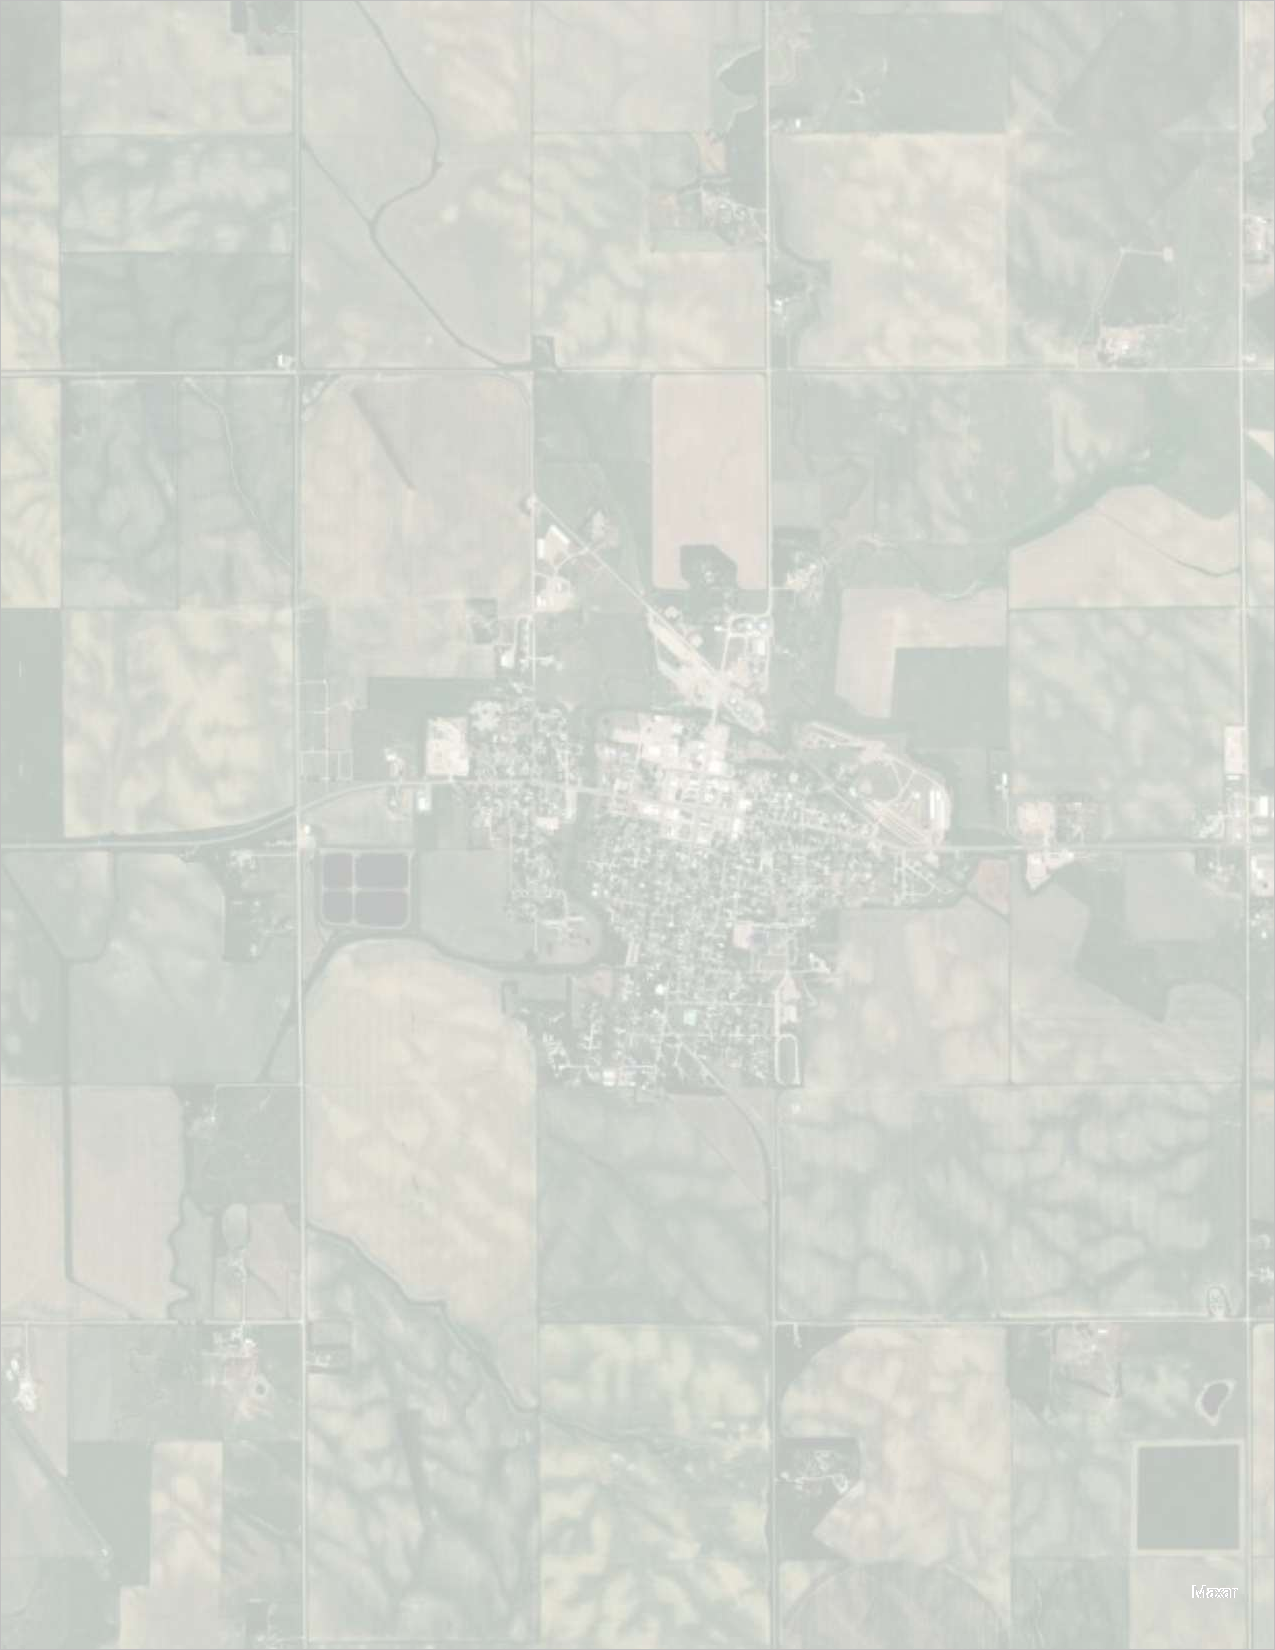
\includegraphics[width=\paperwidth,height=\paperheight]{assets/titlepage_transparent_out.pdf}
  }%
}

\usepackage{pdfpages}

%% Subfigures
\usepackage{subcaption}

%% Multiple columns
\usepackage{multicol}
\usepackage{blindtext}


%% Appendices
\usepackage[title]{appendix}

%%%%% COMPILE DOCUMENT %%%%%
\begin{document}
\pagenumbering{arabic} 
\begin{titlepage}

\BgThispage


\begin{center}

\vspace{2cm}

\includegraphics[width=0.4\textwidth]{assets/five_rule_logo.png}~\\[1cm]
%\vspace{2cm}

%% Title
\hrule
\vspace{.5cm}
{ \huge \bfseries City of Bloomfield Comprehensive Development Plan} % title of the report
\vspace{.5cm}

\hrule
\vspace{1.5cm}

%% Author(s)
\Large
Jordan Duffin Wong, Ph.D\\
\url{jordan@fiveruleplanning.com}\\
2123 Central Ave, Suite D\\
Kearney, Nebraska, 68847

\vspace{2cm}

%% Date
\centering October 2025
\end{center}
\end{titlepage}

\newpage
\doublespacing
%\addcontentsline{toc}{section}{Table of Contents}
\renewcommand{\baselinestretch}{1}\normalsize
\tableofcontents
\renewcommand{\baselinestretch}{1}\normalsize
%\singlespacing
\thispagestyle{empty} % force page style

\newpage
\pagenumbering{arabic} 
\fancyfoot[C]{Page \thepage\ of \pageref{EndOfText}}

%%%%% input pages here %%%%%
\section{Context}

\subsection*{Responsibility to Plan}

\noindent Per \href{https://nebraskalegislature.gov/laws/statutes.php?statute=19-901}{Nebraska Revised Statutes (NRS) \S 19-901(1)}, municipal governments in Nebraska are granted the authority to regulate land use within their jurisdiction:

\begin{quote}
    For the purpose of promoting health, safety, morals, or the general welfare of the community, the city council of a city of the first class or city of the second class or the village board of trustees of a village may adopt zoning regulations which regulate and restrict the height, number of stories, and size of buildings and other structures, the percentage of lots that may be occupied, the size of yards, courts, and other open spaces, the density of population, and the location and use of buildings, structures, and land for trade, industry, residence, or other purposes.
\end{quote}

\subsection*{Authority to Plan}

\noindent \href{https://nebraskalegislature.gov/laws/statutes.php?statute=19-901}{NRS \S 19-901(2)} explains that zoning regulations may not be adopted until a comprehensive plan has been completed, recommended by the Planning Commission, and adopted by the City Council or Village Board of Trustees:

\begin{quote}
    Such powers shall be exercised only after the city council or village board of trustees has established a planning commission, received from its planning commission a recommended comprehensive development plan as defined in section \href{https://nebraskalegislature.gov/laws/statutes.php?statute=19-903}{19-903}, adopted such comprehensive development plan, and received the specific recommendation of the planning commission on the adoption or amendment of zoning regulations. The planning commission shall make a preliminary report and hold public hearings on its recommendations regarding the adoption or repeal of the comprehensive development plan and zoning regulations and shall hold public hearings thereon before submitting its final report to the city council or village board of trustees. Amendments to the comprehensive plan or zoning regulations shall be considered at public hearings before submitting recommendations to the city council or village board of trustees.
\end{quote}

\pagebreak

\noindent A public hearing regarding the recommendation of this Comprehensive Plan was held by the City of Bloomfield \hl{[organization name]} on this date in [year]:\\

\setlength{\hsize}{0.9\hsize}% emphasize effects
\begin{flushright}
\underline{[\,\,\,\,\,\,\,\,\,\,   
            date here     
            \,\,\,\,\,\,\,\,\,\,]
            }
\end{flushright}

\noindent The \hl{[organization name]} recommended the adoption of this Comprehensive on this date in [year]:
\begin{flushright}
\underline{[\,\,\,\,\,\,\,\,\,\,   
            date here     
            \,\,\,\,\,\,\,\,\,\,]
            }
\end{flushright}

\noindent A public hearing regarding the adoption of this Comprehensive Plan was held by the City of Bloomfield \hl{[organization name]} on this date in \hl{[year]}:

\begin{flushright}
\underline{[\,\,\,\,\,\,\,\,\,\,   
            date here     
            \,\,\,\,\,\,\,\,\,\,]
            }
\end{flushright}

\noindent By approving Resolution No. \hl{[resolution number]}, the City of Bloomfield \hl{[organization name]} adopted this Comprehensive Plan on this date in \hl{[year]}:

\begin{flushright}
\underline{[\,\,\,\,\,\,\,\,\,\,   
            date here     
            \,\,\,\,\,\,\,\,\,\,]
            }
\end{flushright}

\pagebreak

\subsection*{Building the Plan}
\noindent The Bloomfield Plan is organized into chapters based upon the guidance and requirements listed within \href{https://nebraskalegislature.gov/laws/statutes.php?statute=19-903}{NRS \S 19-903}:

\begin{quote}
    The regulations and restrictions authorized by sections \href{https://nebraskalegislature.gov/laws/statutes.php?statute=19-901}{19-901} to \href{https://nebraskalegislature.gov/laws/statutes.php?statute=19-915}{19-915} shall be in accordance with a comprehensive development plan which shall consist of both graphic and textual material and shall be designed to accommodate anticipated long-range future growth which shall be based upon documented population and economic projections. The comprehensive development plan shall, among other possible elements, include:
    \begin{enumerate}
        \item [(1)] A land-use element which designates the proposed general distributions, general location, and extent of the uses of land for agriculture, housing, commerce, industry, recreation, education, public buildings and lands, and other categories of public and private use of land;
        \item [(2)] The general location, character, and extent of existing and proposed major roads, streets, and highways, and air and other transportation routes and facilities;
        \item [(3)] The general location, type, capacity, and area served of present and projected or needed community facilities including recreation facilities, schools, libraries, other public buildings, and public utilities and services;
        \item [(4)] When a new comprehensive plan or a full update to an existing comprehensive plan is developed, an energy element which: Assesses energy infrastructure and energy use by sector, including residential, commercial, and industrial sectors; evaluates utilization of renewable energy sources; and promotes energy conservation measures that benefit the community. This subdivision shall not apply to villages; and
        \item [(5)] (a) When next amended after January 1, 1995, an identification of sanitary and improvement districts, subdivisions, industrial tracts, commercial tracts, and other discrete developed areas which are or in the future may be appropriate subjects for annexation and (b) a general review of the standards and qualifications that should be met to enable the municipality to undertake annexation of such areas. Failure of the plan to identify subjects for annexation or to set out standards or qualifications for annexation shall not serve as the basis for any challenge to the validity of an annexation ordinance.
    \end{enumerate}
\end{quote}

\pagebreak
\subsection*{Jurisdiction of the Plan}
\noindent Per \href{https://nebraskalegislature.gov/laws/statutes.php?statute=17-1001}{NRS \S17-1001 (1)}, the geographical area covered by the City of Bloomfield Comprehensive Plan includes all land within a one-mile area encompassing the city, ``the extraterritorial zoning jurisdiction of a city shall consist of the unincorporated area one mile beyond and adjacent to its corporate boundaries."\\

\noindent \textbf{Bloomfield Boundary and Extraterritorial Jurisdiction} on the following page displays Bloomfield's corporate boundary and zoning jurisdiction, which includes all lands within the City of Bloomfield and its One-Mile Extraterritorial Jurisdiction (ETJ). Bloomfield's land use policies govern all lands within the city as well as the ETJ.\\

\noindent The map on the next page, \textbf{\textcolor{coBalt}{Bloomfield Municipal Boundary and Extraterritorial Jurisdiction}}, shows the extent of this territory. All\footnote{Other territories, such as Bloomfield Community Schools, expand beyond the ETJ. They will be included as necessary context for the plan, but are not (necessarily) subject to the emphasis on future land use planning.} of the existing and future land use decisions will be made with respect to this geographic footprint.

\pagebreak
\begin{landscape}
    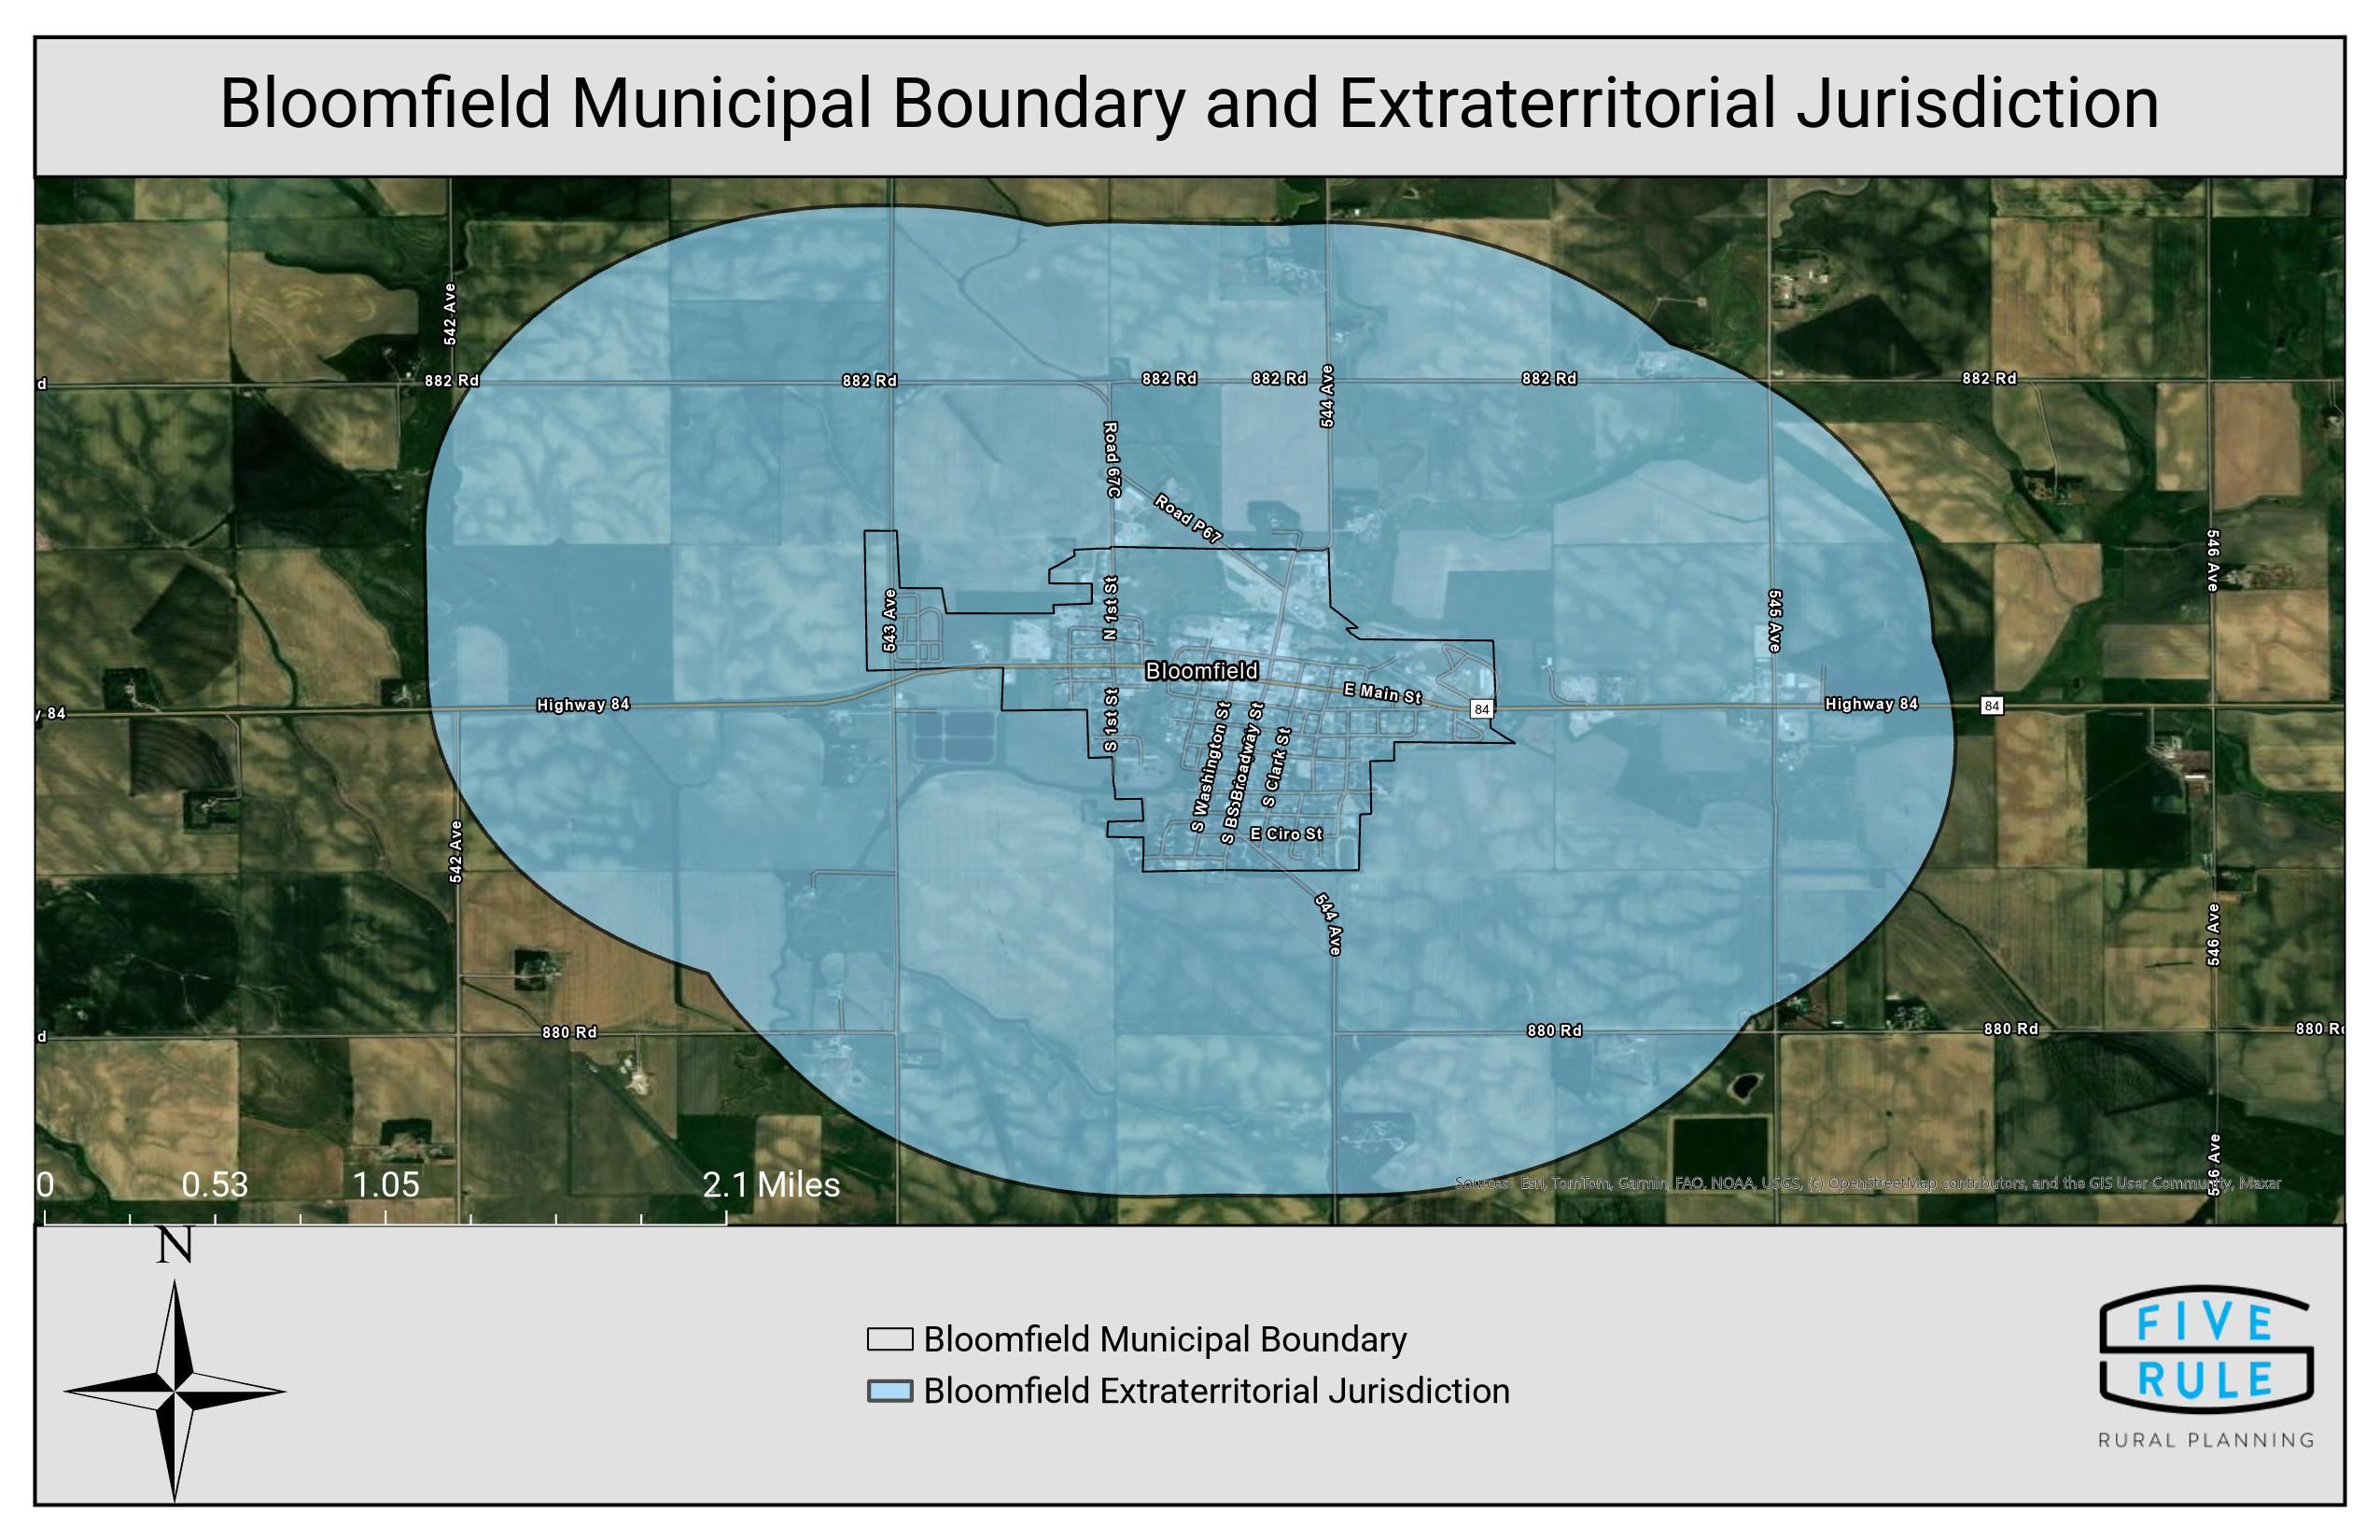
\includepdf[angle=90]{maps/boundary_etj.pdf}
\end{landscape}
\pagebreak
\pagebreak
\section{Existing Land Use}

\noindent The existing land use (ELU) map provides a visual representation of how land in Bloomfield is currently being utilized. It is a snapshot of the current state of the city's existing land use patterns and helps with the decision-making processes related to land development, zoning regulation, and infrastructure funding.\\

\noindent The ELU map categorizes different areas -- typically parcels of land -- based on their primary uses today. It assists with identifying areas of change or potential growth, as well as with making informed decisions about future development and zoning regulations.\\

\begin{table}[H] 
\begin{framed}
\centering \doublespacing
  \caption{Bloomfield Existing Land Use Inventory}
  \label{table:landUseInventory}
 \scalebox{1.00}{
\begin{tabular}{l D{.}{.}{8.5} D{.}{.}{8.5} D{.}{.}{8.5}} \hline
& \multicolumn{3}{c}{\textbf{Within Bloomfield City Limits}} \\
\hline \hline
& \multicolumn{1}{c}{Parcels} & \multicolumn{1}{c}{Area}  & \multicolumn{1}{c}{Percent of Total Area}  \\ \hline
Agricultural        & 14    & 0.042     & 6.49\%  \\
Commercial          & 117   & 0.101     & 15.62\% \\
Residential         & 519   & 0.342     & 52.87\% \\
Exempt              & 95    & 0.162     & 25.02\% \\
\hline \hline
& \multicolumn{3}{c}{\textbf{Within Bloomfield Extraterritorial Jurisdiction}} \\
\hline \hline
& \multicolumn{1}{c}{Parcels} & \multicolumn{1}{c}{Area}  & \multicolumn{1}{c}{Percent of Total Area}  \\ \hline
Agricultural        & 72    & 7.136     & 86.58\% \\
Commercial          & 129   & 0.190     & 2.31\%  \\
Residential         & 536   & 0.363     & 4.41\%  \\
Exempt              & 114   & 0.553     & 6.71\%  \\
\hline \hline
\end{tabular}
}
\floatnote{All geographic units are in square miles. Data come from the Knox County Property Assessor and the \href{https://www.census.gov/geographies/mapping-files/time-series/geo/tiger-line-file.html}{2022 U.S. TIGER/Line Shapefiles}.}
\end{framed}
\end{table}

\pagebreak
\noindent \textbf{Table~\ref{table:landUseInventory}} breaks down the distribution of parcels in Bloomfield by land use. There are four categories: agricultural, commercial, residential, and exempt. Within city limits, residential properties make up just over half of all land area, while exempt (primarily public-use) properties make up about one quarter, and commercial properties make up about fifteen percent. Very little of the area within city limits sees agricultural use.

\subsection*{One-Mile Zoning Jurisdiction}

\noindent Residents and landowners located outside of the corporate limits but within one mile do not elect city officials nor pay property tax to the city. Nonetheless, these lands are important to the city's future for several reasons:

\begin{itemize}
    \item [(1)] \textbf{Growth and Expansion}: Planning for these adjacent lands will allow the city to make decisions with future growth and expansion plans in mind. As Bloomfield grows, it will annex nearby lands to meet the necessary demand for housing, infrastructure, and services.
    \item [(2)] \textbf{Infrastructure and Utilities}: Planning ahead and deciding how the city will most likely grow helps with efficiently extending existing infrastructure to include water and sanitary extensions, as well as connected street networks.
    \item [(3)] \textbf{Economic Development}: The city's adjacent lands will be needed to support the expansion and recruitment of businesses and industries providing services, goods, and jobs.
    \item [(4)] \textbf{Environmental Considerations}: Cities need to consider the environmental impact of adjacent lands. Planning can help identify areas with ecological value, sensitive habitats, or natural resources that should be protected from inappropriate development. It allows cities to implement measures for sustainable land management, conservation, and mitigation of potential environmental risks.
\end{itemize}

\noindent For these reasons, the lands located outside of Bloomfield but within the one-mile zoning jurisdiction are also inventoried. \textbf{Table~\ref{table:landUseInventory}} also summarises this land use, the vast majority (87 percent) of which is used agriculturally. Small percentages of the land are designated exempt (6.71 percent), residential (4.41 percent), or commercial (2.31 percent).

\newpage
\thispagestyle{empty}
\begin{landscape}
    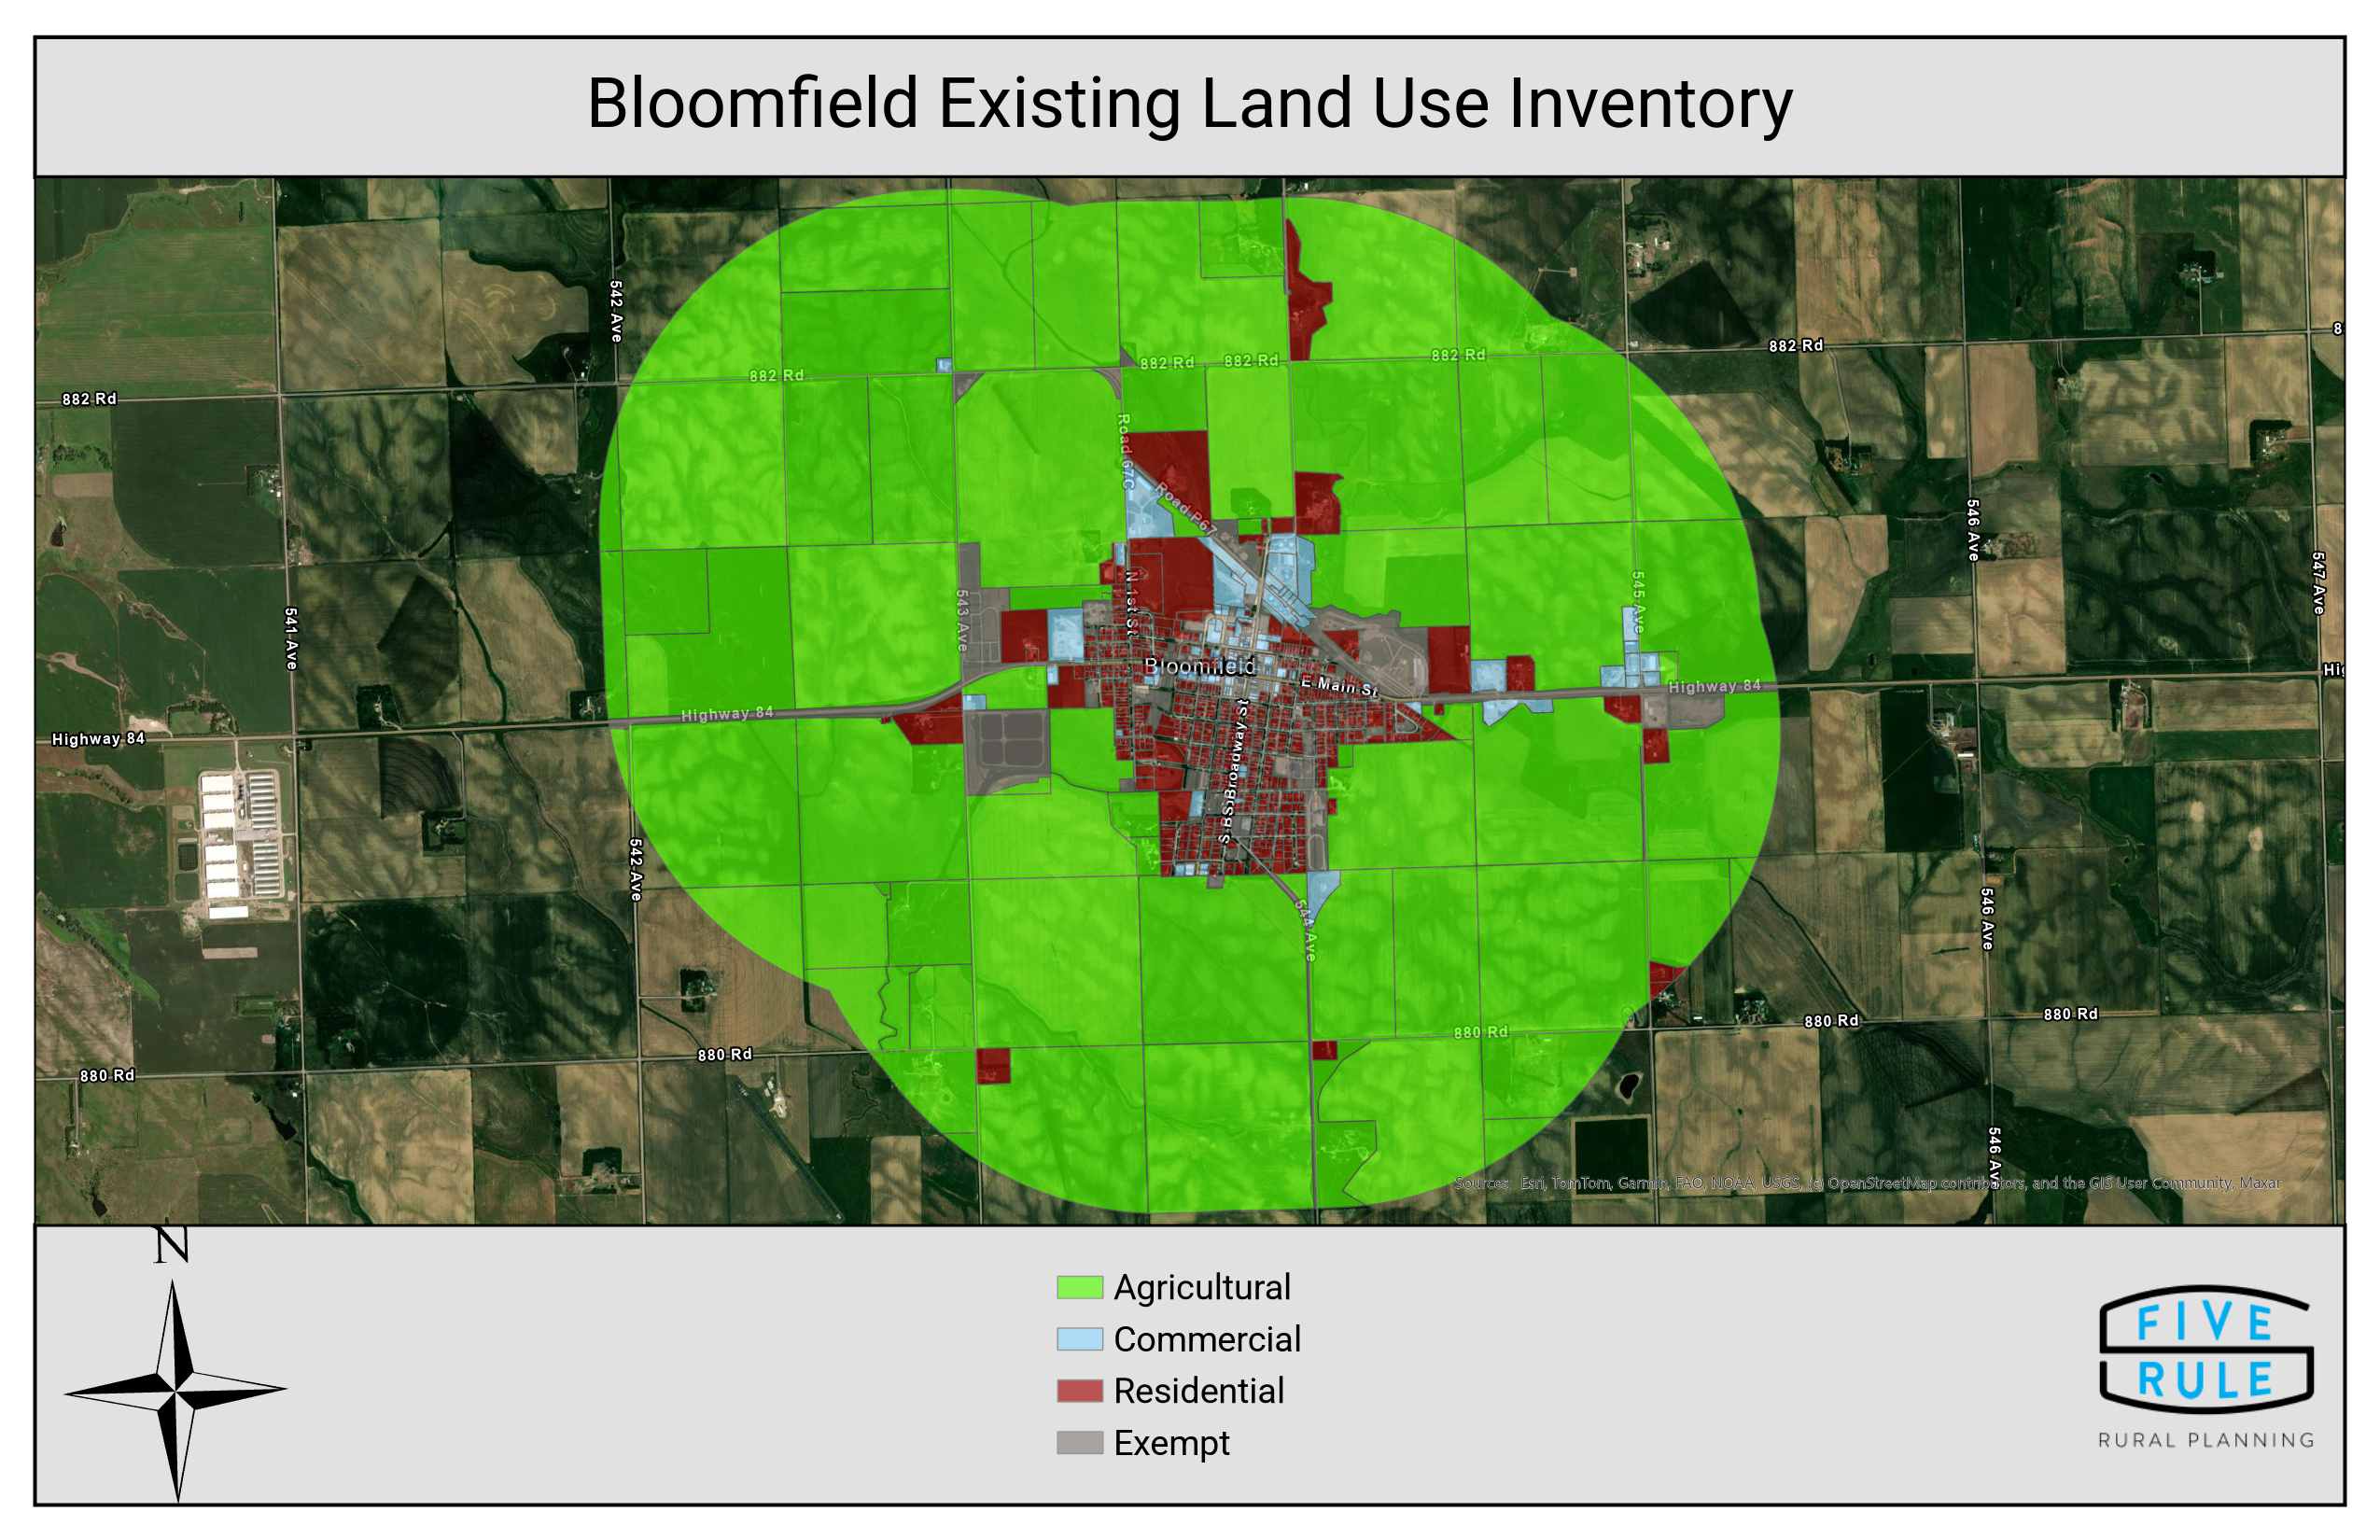
\includepdf[angle = 90]{maps/ELU.pdf}
\end{landscape}
\pagebreak
\section{Housing Assessment}

\noindent In this chapter, we document the condition, status, and needs for housing in Bloomfield. Drawing on a variety of data from the Knox County Property Assessor, various government agencies, and an original survey of Bloomfield residents, we show that Bloomfield has a long-term trend of population decline and housing structures in need of improvement. Amidst this, Bloomfield has the challenge of supporting affordable housing development while supplying amenities -- particularly childcare -- to encourage existing young families to stay in Bloomfield and new ones to move there.

\subsection{Condition of Housing Structures}

\noindent The status and condition of structures are categorized by the Knox County property assessor. \textbf{Table~\ref{table:landConditionRes}} shows how the assessor has rated these parcels in Bloomfield:

\begin{table}[H] 
\begin{framed}
\centering \doublespacing
  \caption{Bloomfield Residential Land Use Conditions}
  \label{table:landConditionRes}
 \scalebox{0.95}{
\begin{tabular}{l D{.}{.}{8.5} D{.}{.}{8.5} D{.}{.}{8.5}}
\hline \hline
& \multicolumn{1}{c}{Parcels} & \multicolumn{1}{c}{Percent of Total Parcels}  & \multicolumn{1}{c}{Perecnt of Total Area}  \\ \hline
Worn-Out                & 2     & 0.46\%    & 0.27\%    \\
Worn-Out - Badly Worn   & 2     & 0.46\%    & 0.19\%    \\
Badly Worn              & 23    & 5.29\%    & 3.58\%    \\
Badly Worn - Average    & 32    & 7.36\%    & 6.47\%    \\
Average                 & 315   & 72.41\%   & 74.99\%   \\
Average - Good          & 42    & 9.66\%    & 9.94\%    \\
Good                    & 18    & 4.14\%    & 4.00\%    \\
Good - Very Good        & 1     & 0.23\%    & 0.57\%    \\
Very Good               & 0     & 0.00\%    & 0.00\%    \\
\hline
\end{tabular}
}
\floatnote{Area units are in square miles. Data come from the Knox County Property Assessor.}
\end{framed}
\end{table}

\pagebreak
\subsubsection*{Remarks on Housing Conditions}
\begin{itemize}
    \item [(1)] \textbf{\textcolor{coBalt}{Majority of Housing is in Average Condition}}
    \begin{itemize}
        \item The most common rating for residential structures in Bloomfield is "average," indicating that:
        \begin{itemize}
            \item The majority of homes are habitable and maintain a standard level of functionality.
            \item However, they may lack modern updates or show signs of aging and general wear.
        \end{itemize}
        \item This suggests stable but aging housing stock, which may require investment in maintenance or modernization over the next decade.
    \end{itemize}
    \item [(2)] \textbf{\textcolor{coBalt}{Minimal "Worn-Out" Properties}}
    \begin{itemize}
        \item Less than one percent of homes are considered "Worn-Out," meaning:
        \begin{itemize}
            \item Very few homes are in a state of severe disrepair or uninhabitable condition.
            \item This reflects basic housing adequacy across the city, with little evidence of total structural abandonment.
            \item It also suggests that code enforcement or demolition efforts may be effective in preventing blight at the extreme end.
        \end{itemize}
    \end{itemize}
    \item [(3)] \textbf{\textcolor{coBalt}{Significant Proportion of "Badly Worn" Housing}}
    \begin{itemize}
        \item About 13\% of the housing stock is "Badly Worn, "which is a red flag:
        \begin{itemize}
            \item These homes may have serious deficiencies in systems (roofing, plumbing, electrical, foundation) or visible deterioration.
            \item This group likely represents homes that are still occupied but nearing the point where repairs or renovations are critical.
            \item This condition group is the most at-risk of becoming "Worn-Out" without intervention.
        \end{itemize}
    \end{itemize}
    \item [(4)] \textbf{\textcolor{coBalt}{Limited "Good" Condition Properties}}
    \begin{itemize}
        \item Only four percent of houses are rated as "Good" or better
        \begin{itemize}
            \item There is a small segment of housing stock that is newer, well-maintained, or recently renovated
            \item This could indicate limited recent investment in high-quality residential development or upgrades
            \item It may also highlight the need for incentives to support home improvement or new builds.
        \end{itemize}
    \end{itemize}
    \pagebreak
    \item [(5)] \textbf{\textcolor{coBalt}{Overall Implications for Housing Policy}}
    \begin{itemize}
        \item The data paint a picture of a largely functional housing stock, but one that is aging and moderately deteriorated.
        \item The low percentage of "Good" homes and the notable share of "Badly Worn" ones suggest thatBloomfield may benefit from target housing rehabilitation programs, especially for owner-occupied homes in poor condition.
        \item Grant funding and development efforts could be focused on preventing the decline of average-rated homes while prioritizing repairs for the 13\% Badly Worn stock.
    \end{itemize}
\end{itemize}

\newpage
\thispagestyle{empty}
\begin{landscape}
    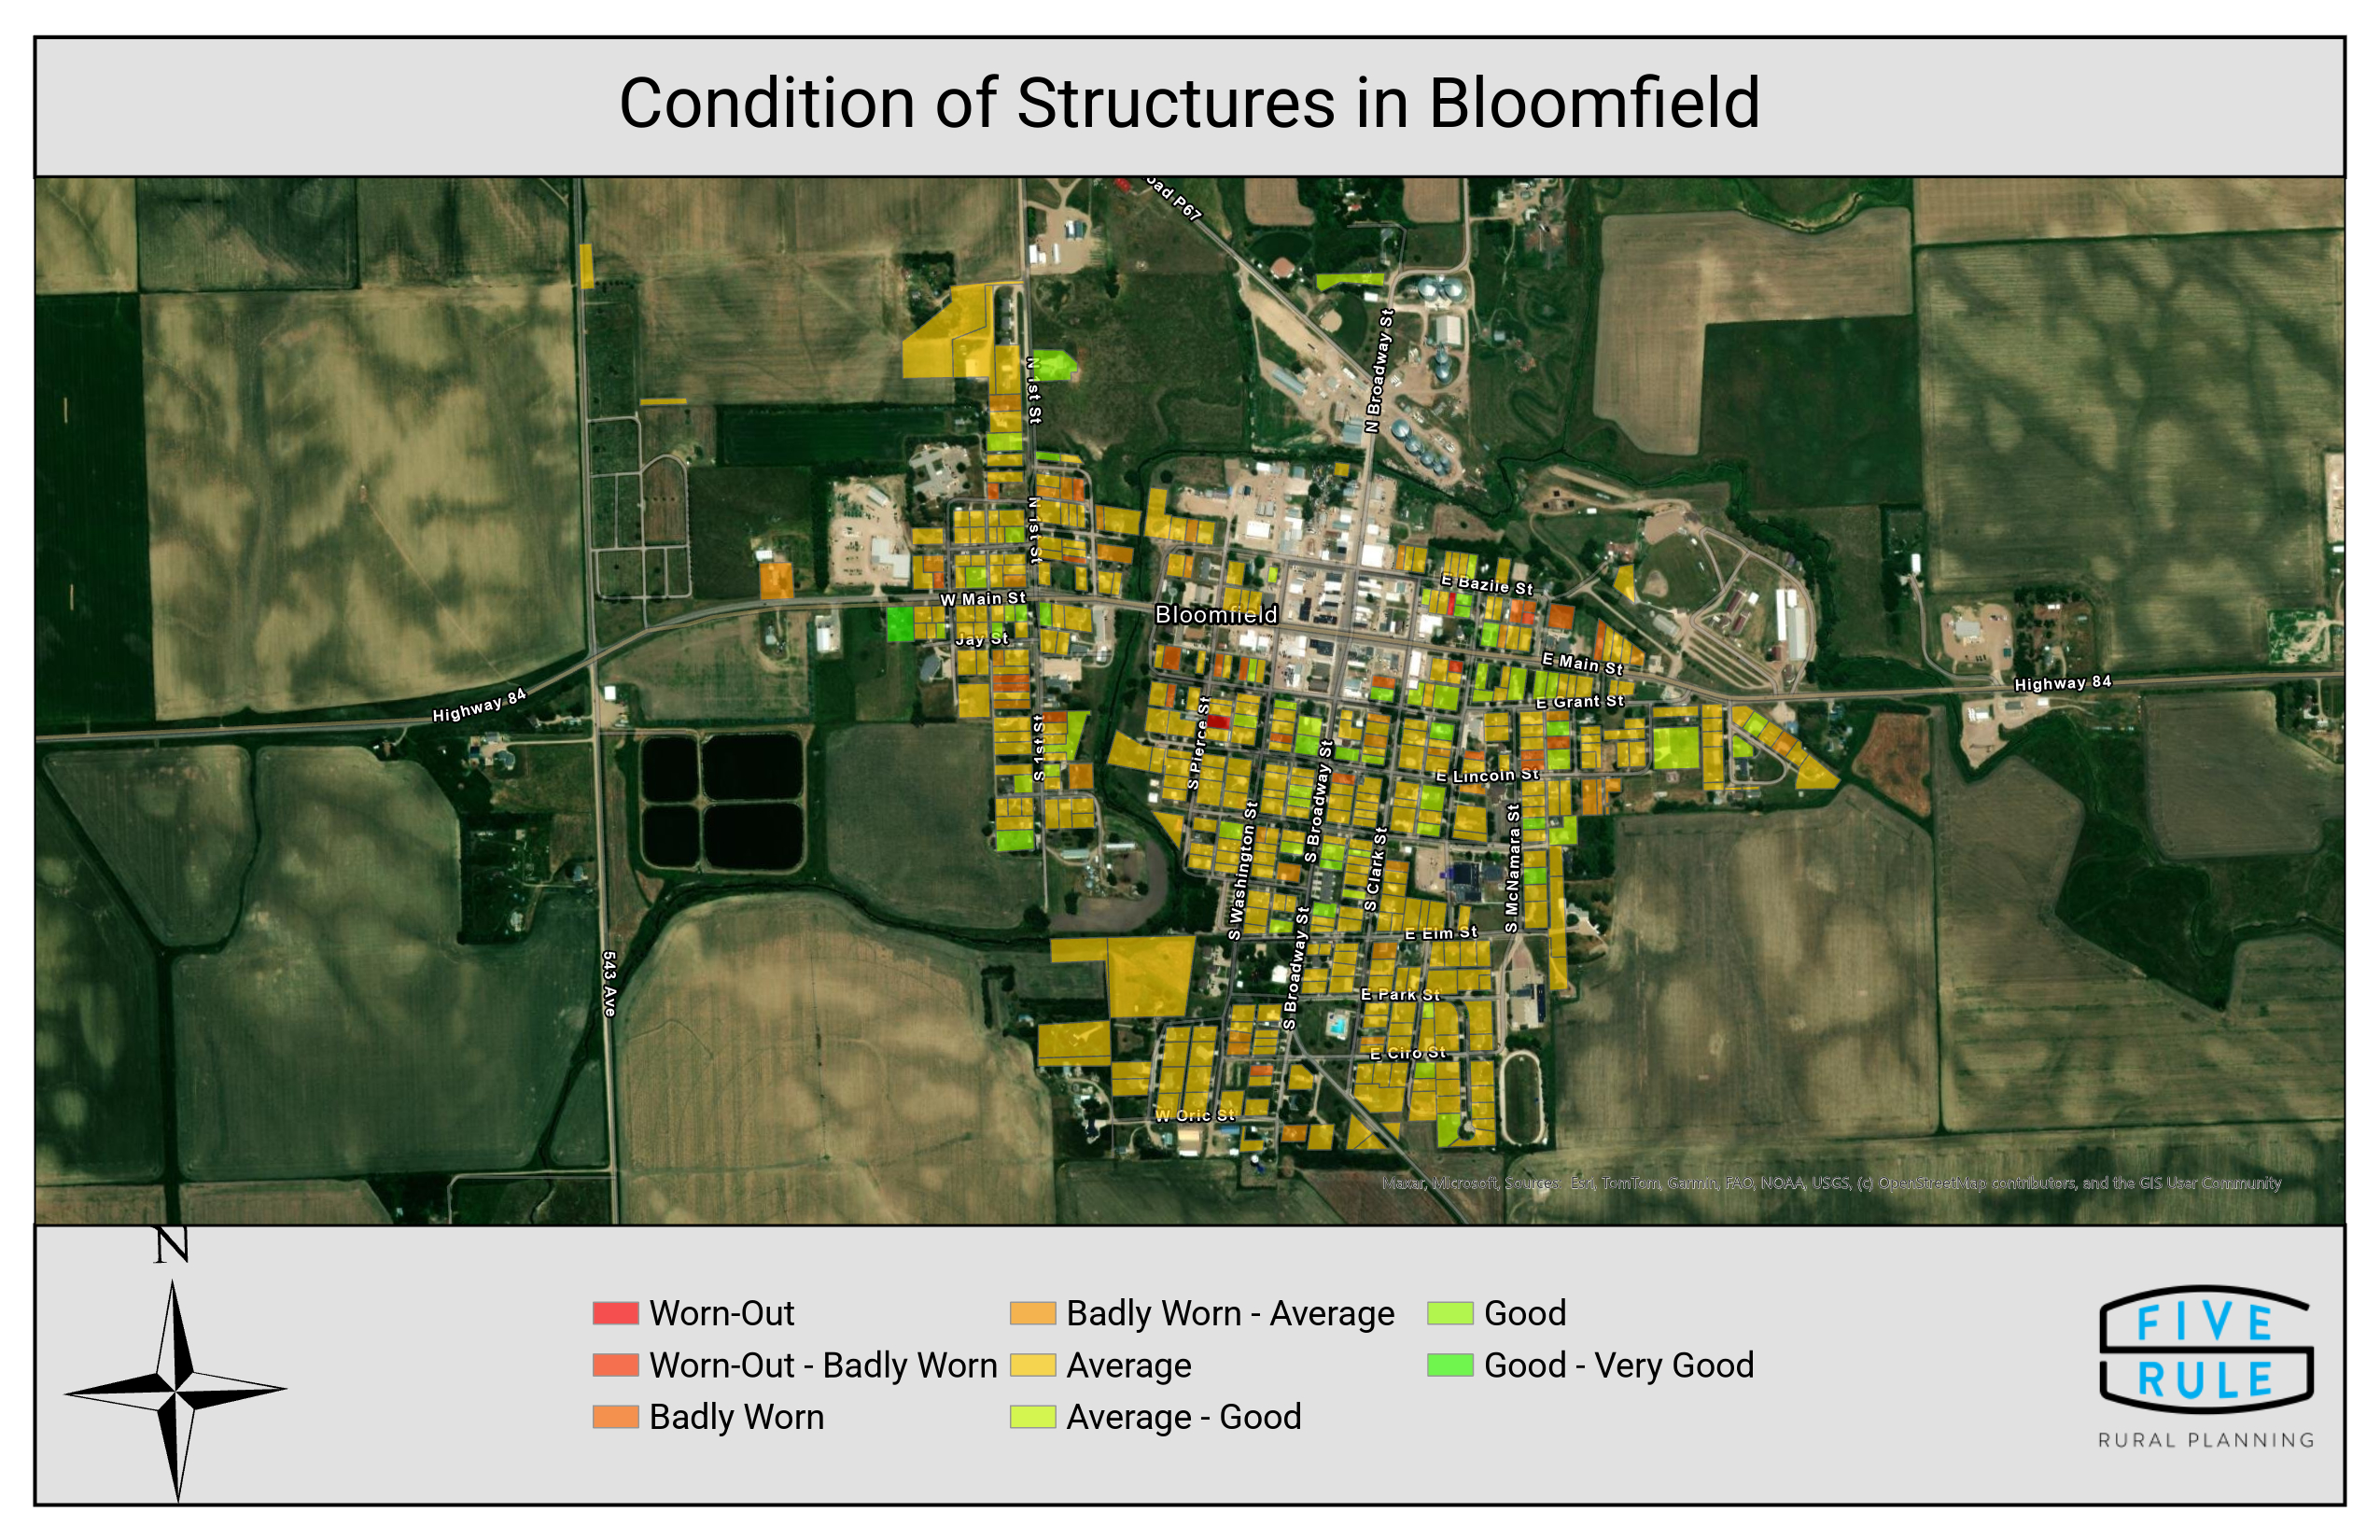
\includepdf[angle = 90]{maps/structure_conditions.pdf}
\end{landscape}
\newpage

\noindent The ages of structures are categorized by the Knox County property assessor. \textbf{Table~\ref{table:landAgeRes}} shows the age distribution of structures in Bloomfield.\\

\begin{table}[H] 
\begin{framed}
\centering \doublespacing
  \caption{Bloomfield Residential Land Use Age}
  \label{table:landAgeRes}
 \scalebox{0.95}{
\begin{tabular}{l D{.}{.}{8.5} D{.}{.}{8.5} D{.}{.}{8.5}}
\hline \hline
\multicolumn{1}{c}{Era Built} & \multicolumn{1}{c}{Parcels} & \multicolumn{1}{c}{Percent of Total Parcels}  & \multicolumn{1}{c}{Perecnt of Total Area}  \\ \hline
Before 1900 & 37    & 8.51\%    & 8.06\%    \\
1900-1920   & 157   & 36.10\%   & 35.56\%   \\
1920-1940   & 26    & 5.98\%    & 4.40\%    \\
1940-1960   & 53    & 12.18\%   & 9.36\%    \\
1960-1980   & 118   & 27.18\%   & 27.03\%   \\
1980-2000   & 36    & 8.28\%    & 11.91\%   \\
2000-2020   & 8     & 1.84\%    & 3.67\%    \\
After 2020  & 0     & 0.00\%    & 0.00\%    \\
\hline
\end{tabular}
}
\floatnote{Area units are in square miles. Data come from the Knox County Property Assessor.}
\end{framed}
\end{table}

\pagebreak
\subsubsection*{Remarks on Housing Age}
\begin{itemize}
    \item [(1)] \textbf{\textcolor{coBalt}{Dominance of Early 20th-Century Homes}}
    \begin{itemize}
        \item A large share of Bloomfield's housing stock was built between 1900 and 1960 (63\%).
        \item The most-represented period is \textbf{1900-1920 (36\%)}.
        \item The fact that many homes are more then one-hundred years old indicates a large need for \textbf{ongoing maintenance and potential rehabilitation}.
    \end{itemize}
    \item [(2)] \textbf{\textcolor{coBalt}{Prevalance of Pre-1900 homes}}
    \begin{itemize}
        \item 37 homes were built before 1900 (8.51\%).
        \item These homes represent \textbf{historic structures}, often requiring specialized upkeep and are possibly eligible for \textbf{preservation incentives}.
    \end{itemize}
    \item [(3)] \textbf{\textcolor{coBalt}{Mid-Century Infill}}
    \begin{itemize}
        \item Significant housing construction took place \textbf{1960 and 1980}, with \textbf{118 units built}.
        \item These homes are typically more modern in layout and materials, and \textbf{tend to be located away from Bloomfield's downtown}.
    \end{itemize}
    \item [(4)] \textbf{\textcolor{coBalt}{Minimal 21st-Century Construction}}
    \begin{itemize}
        \item Only 8 units have been built since 2000.
        \item This indicates lower levels of new development, possible barriers such as \textbf{land availability, economic constraints, or infrastructure limitations}, and a need for \textbf{housing investment or incentives} to encourage new construction.
    \end{itemize}
    \item [(5)] \textbf{\textcolor{coBalt}{Overall Implications for Housing Policy}}
    \begin{itemize}
        \item Bloomfield's housing inventory is largely composed of \textbf{century-old homes}, with litte recent development.
        \item This indicates a \textbf{mature and aging housnig stock}, suggesting a need for \textbf{housing rehabilitation programs}, targeted infill development, \textbf{infrastructure upgrades} to support new residential construction, and \textbf{strategic programming} to preserve historic character while meeting modern housing needs.
    \end{itemize}
\end{itemize}


\newpage
\thispagestyle{empty}
\begin{landscape}
    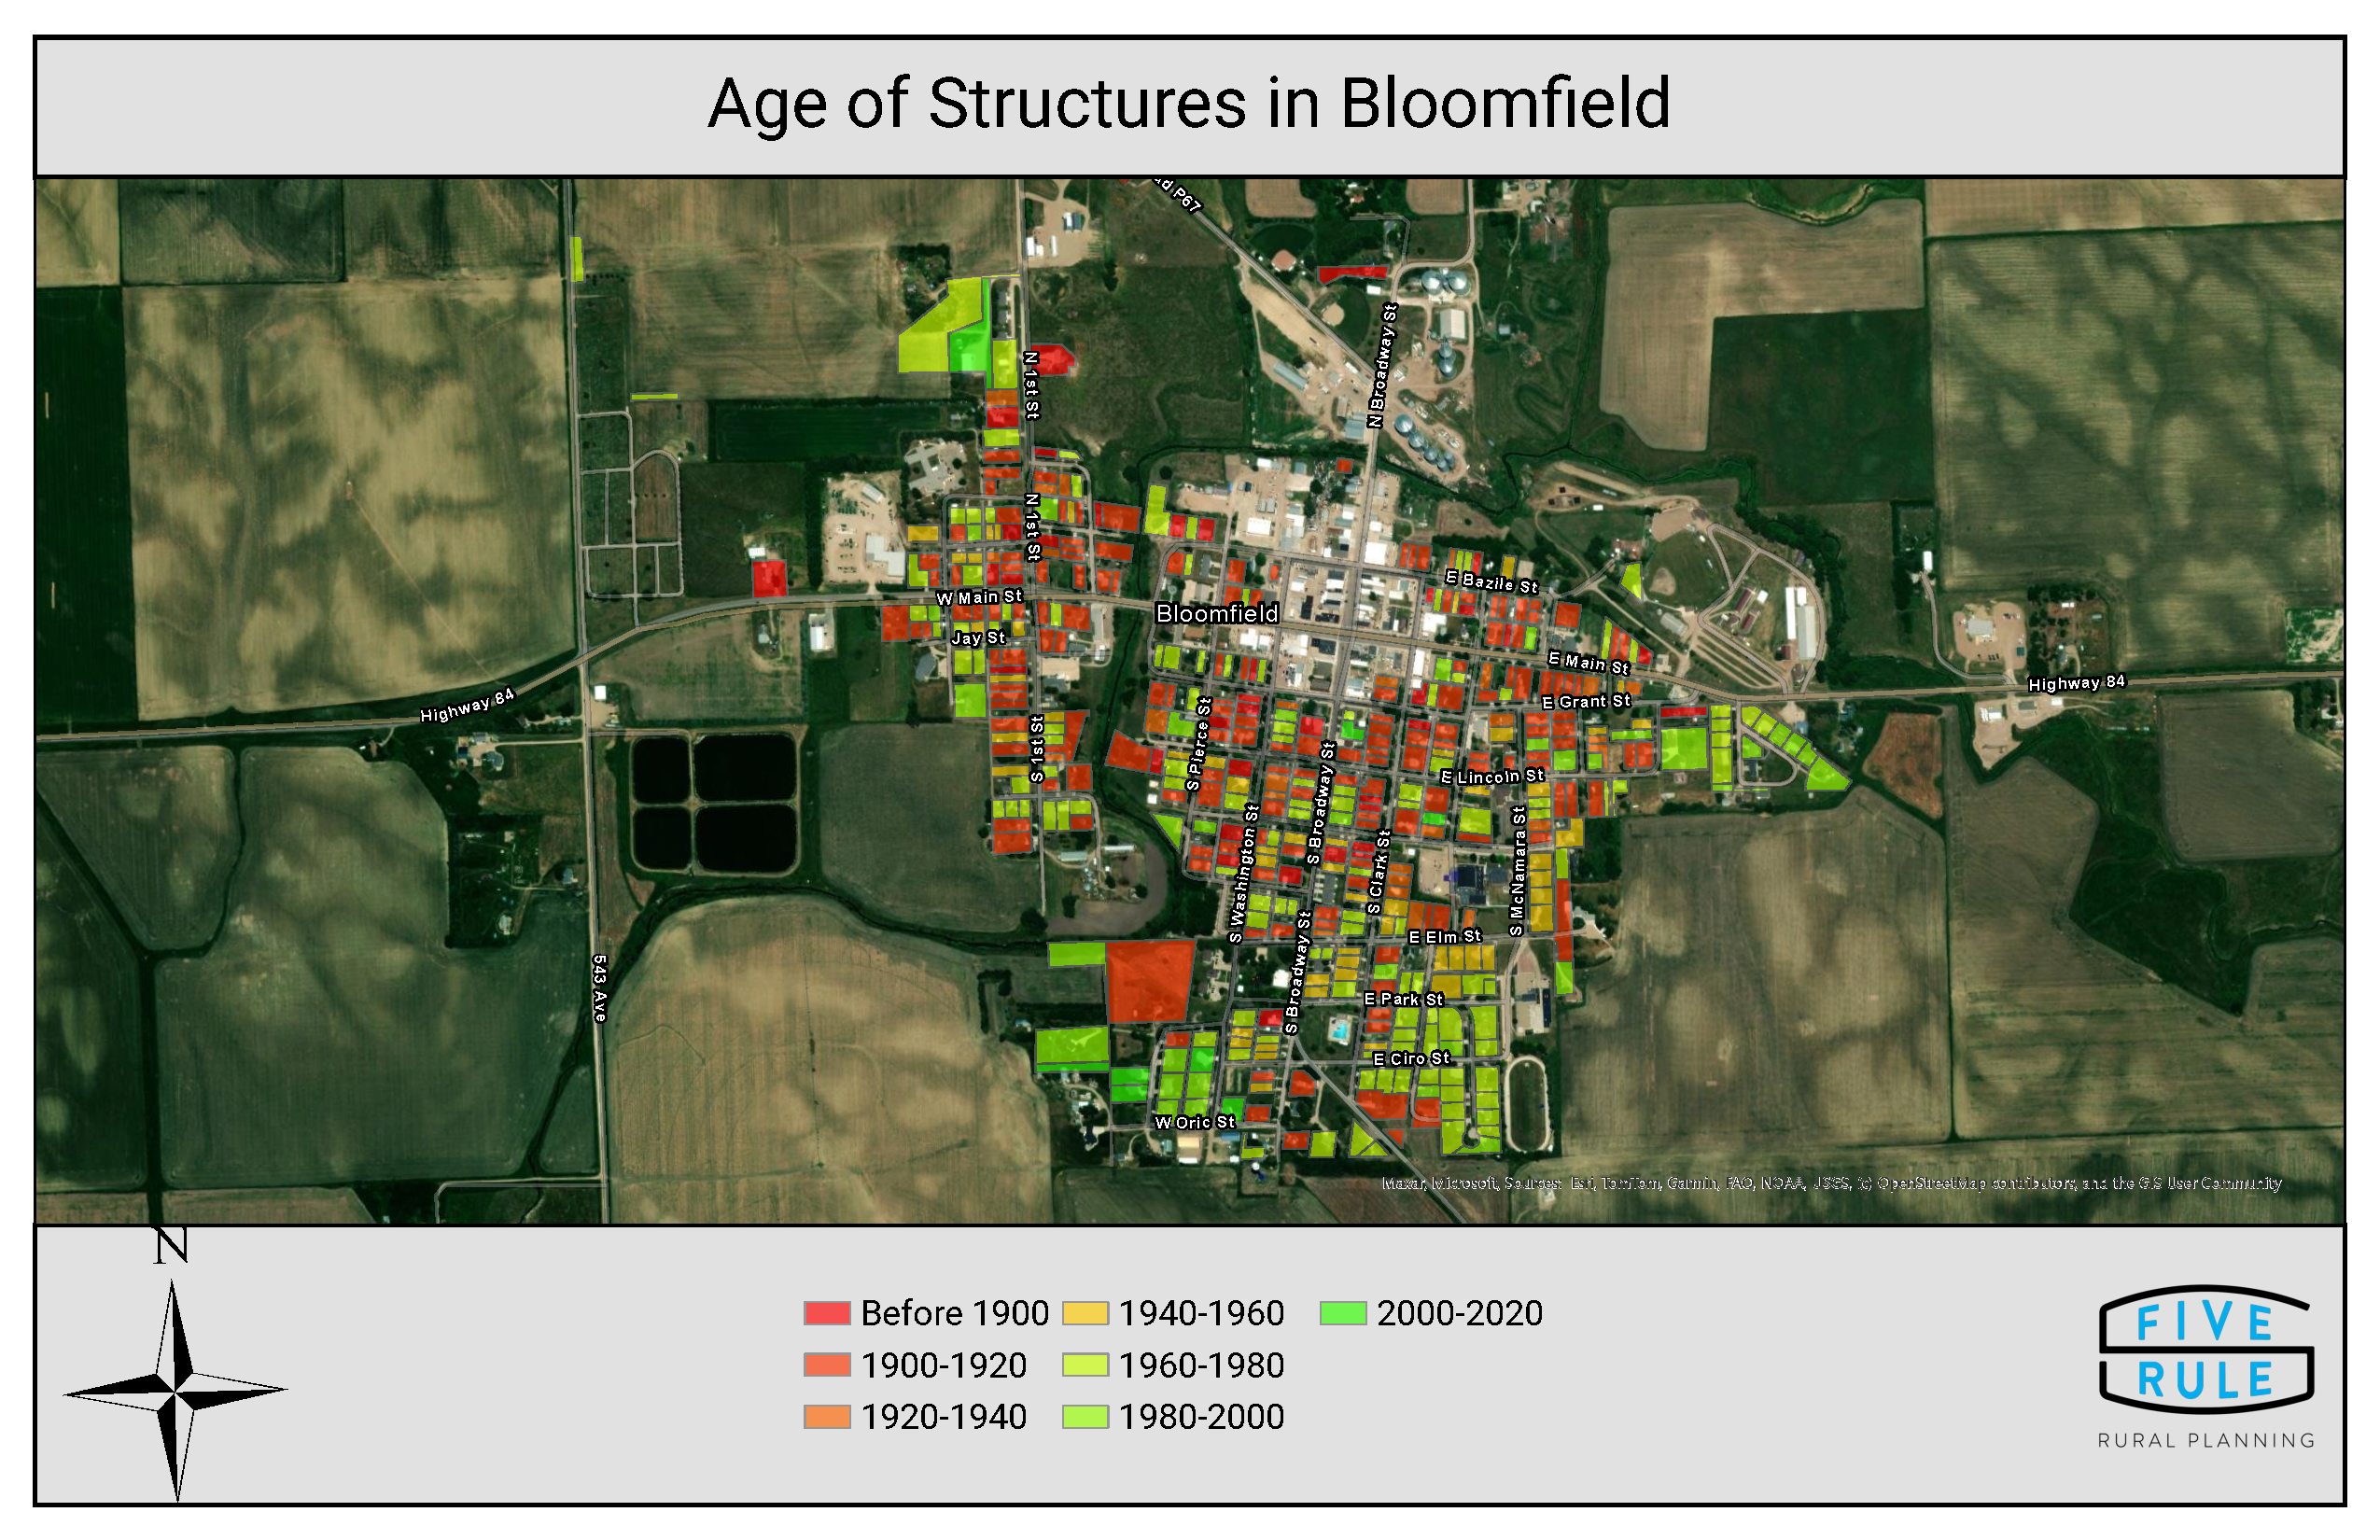
\includepdf[angle = 90]{maps/structure_age.pdf}
\end{landscape}
\newpage

\pagebreak
\subsection{Vacant and Underutilized Properties}
\noindent \hl{[waiting on Scot and Brad to get back to us]}

\pagebreak
\subsection{Community Housing Needs}

% \subsubsection{Historic Population Growth and Decline}

\noindent \textbf{Figure~\ref{fig:historicPop}} shows how Bloomfield's population has changed over the last century. The city population peaked in the 1940s and experienced a smaller bump in the 1970s before beginning to steadily decline to just under 1,000 residents today. The decline was most pronounced in the 1990s.

\begin{figure}[H]
\centering
\begin{framed}
    \caption{Historic Population Growth and Decline}
    \label{fig:historicPop}
    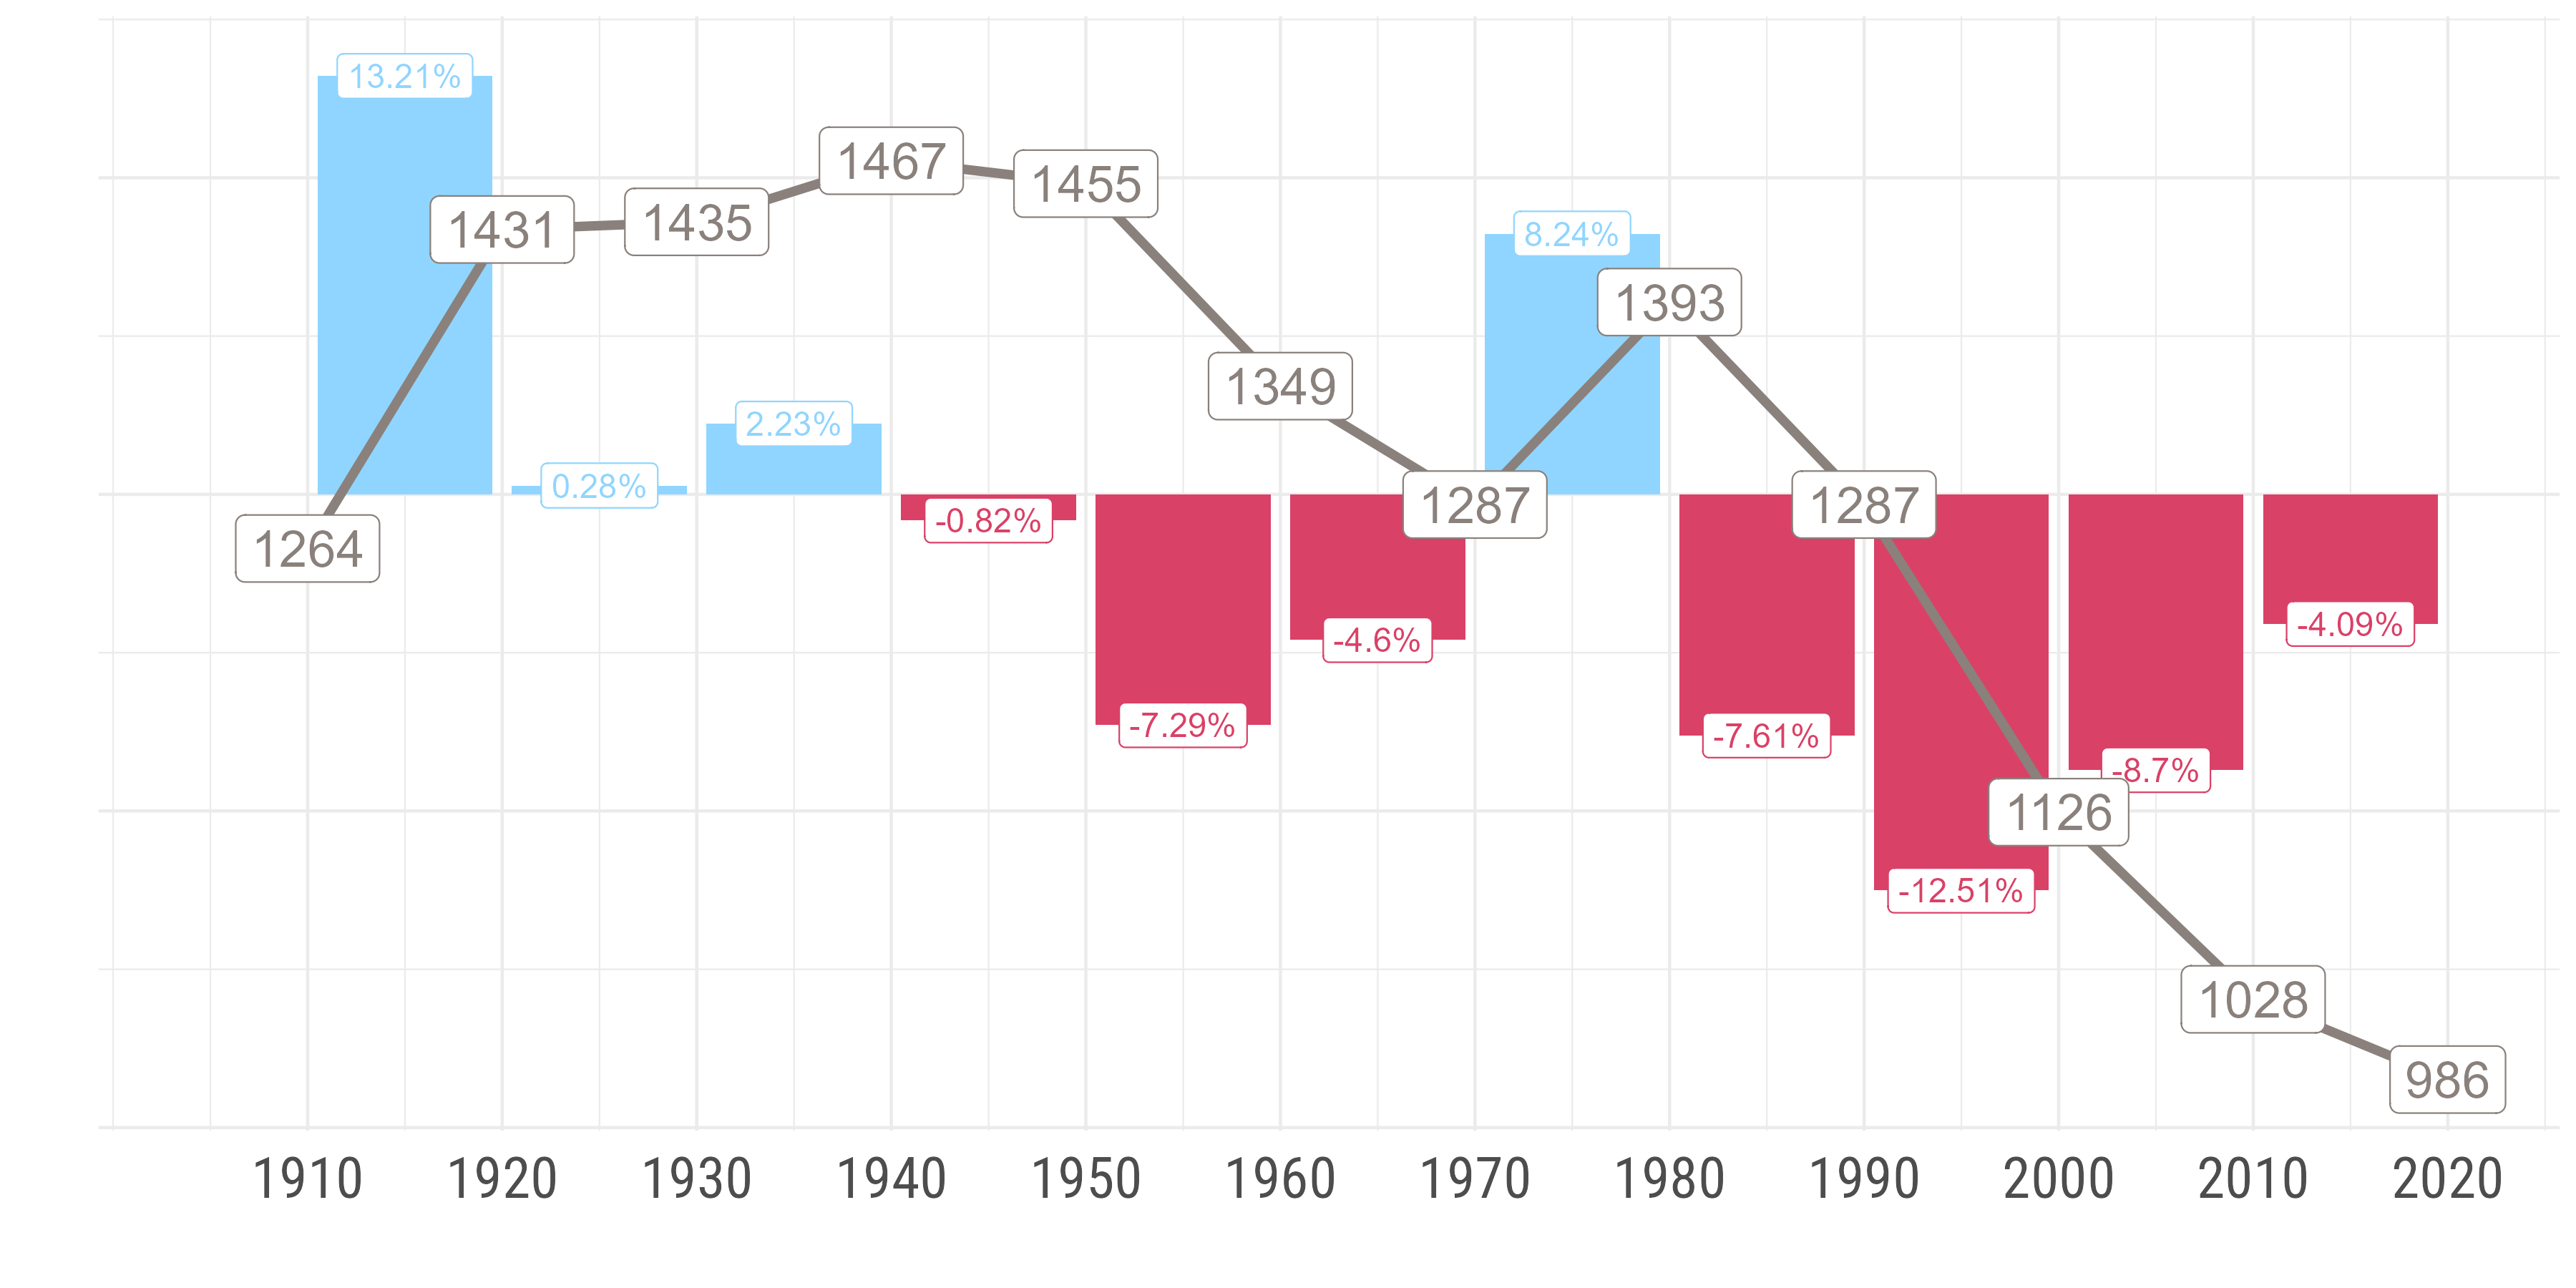
\includegraphics[width=\linewidth]{figures/historical_population_trends.png}
    \rule[-5pt]{\linewidth}{0.4pt}
    \floatnote{Data come from the \href{https://www.unomaha.edu/college-of-public-affairs-and-community-service/center-for-public-affairs-research/programs/nebraska-state-data-center.phpl}{University of Nebraska-Omaha Data Center} and the \href{https://www.census.gov/programs-surveys/decennial-census.html}{Decennial Census}.}
\end{framed}
\end{figure}

% \subsection{Population Projections}

\noindent \textbf{Figure~\ref{fig:populationProjections}} presents several possible population scenarios for Bloomfield. There are many unknown factors that can affect future growth projections. However, many organizations rely on using historical trends as the basis for forecasting future growth or decline.\\

\begin{figure}[H]
\centering
\begin{framed}
    \caption{Population Projections for Bloomfield, Nebraska}
    \label{fig:populationProjections}
    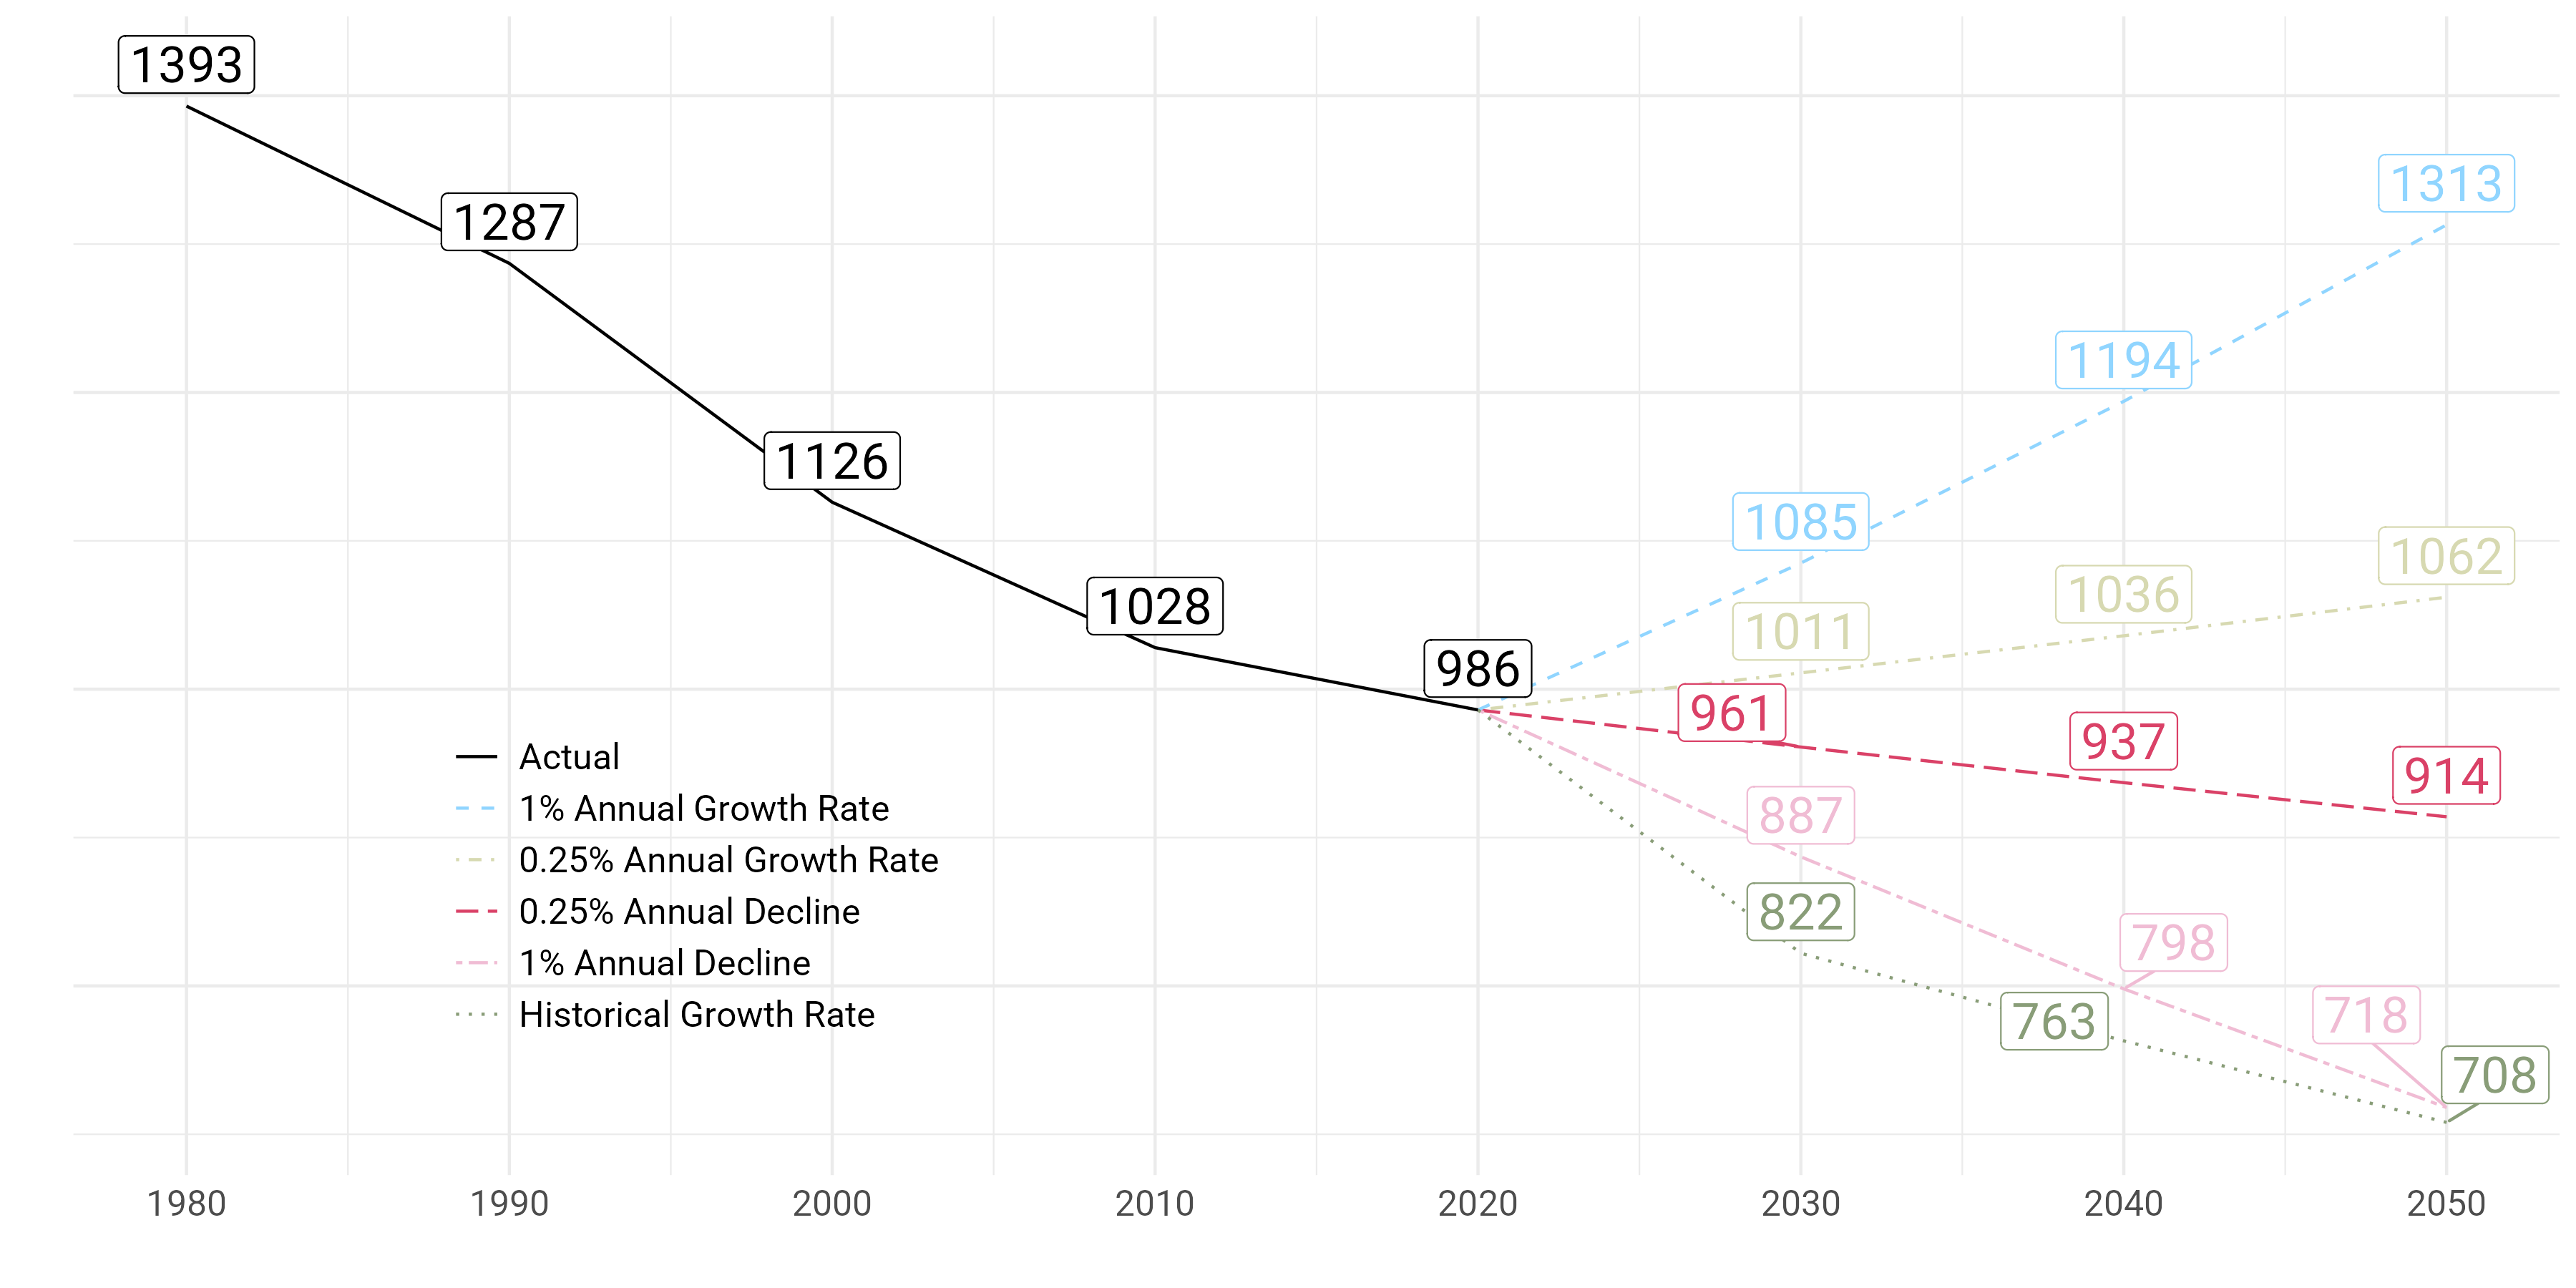
\includegraphics[width=\linewidth]{figures/population_projections.png}
    \rule[-5pt]{\linewidth}{0.4pt}
    \floatnote{Data come from the \href{https://www.unomaha.edu/college-of-public-affairs-and-community-service/center-for-public-affairs-research/programs/nebraska-state-data-center.phpl}{University of Nebraska-Omaha Data Center} and the \href{https://www.census.gov/programs-surveys/decennial-census.html}{Decennial Census}.}
\end{framed}
\end{figure}

\noindent Some projections indicate future growth for Bloomfield, while others -- including the historical one -- suggest continued decline. However, if Bloomfield's population grows, the city will need to add additional housing units. This will require the new development of adjacent lands and possible redevelopment of lands already in the city. \textbf{Table~\ref{table:populationProjections}} uses the 2023 ACS estimate of 2.04 persons per household to document projected needs.

\begin{table}[H] 
\begin{framed}
\centering \doublespacing
  \caption{Population Projection Scenarios and Housing Needs}
  \label{table:populationProjections}
 \scalebox{0.85}{
\begin{tabular}{l D{.}{.}{8.5} D{.}{.}{8.5}}
\hline \hline
& \multicolumn{1}{c}{\textbf{0.25\% Annual Growth Rate}} & \multicolumn{1}{c}{\textbf{1\% Annual Growth Rate}} \\ \hline
2040 Population Projection          & 1036  & 1194  \\
2050 Population Projection          & 1062  & 1313  \\
Total Population Increase by 2050   & 76    & 327   \\ \hline
New Housing Units Needed by 2050    & 38    & 161   \\
\hline
\end{tabular}
}
\floatnote{Data come from the \href{https://www.unomaha.edu/college-of-public-affairs-and-community-service/center-for-public-affairs-research/programs/nebraska-state-data-center.phpl}{University of Nebraska-Omaha Data Center}, the \href{https://www.census.gov/programs-surveys/decennial-census.html}{Decennial Census}, and the \href{https://www.census.gov/programs-surveys/acs.html}{2023 American Community Survey Five-Year Estimates}.}
\end{framed}
\end{table}

\pagebreak
\subsubsection*{Families and Households}
\noindent The Census defines a \textbf{family} as any two or more people (not necessarily including a householder) residing together and related by birth, marriage, or adoption. A \textbf{household} consists of one or more persons residing together who may or may not be related by birth, marriage, or adoption. Multiple families can reside in the same household.\\

\noindent \textbf{Figure~\ref{fig:householdSize}} is based on estimates from the 2023 U.S. Census American Community Survey and shows how average family and household sizes have changed in Bloomfield over the past decade. The average family size has fluctuated but is now about the same as it was a decade prior, while the average household size has generally increased.

\begin{figure}[H]
\centering
\begin{framed}
    \caption{Average Family and Household Sizes, 2013-2023}
    \label{fig:householdSize}
    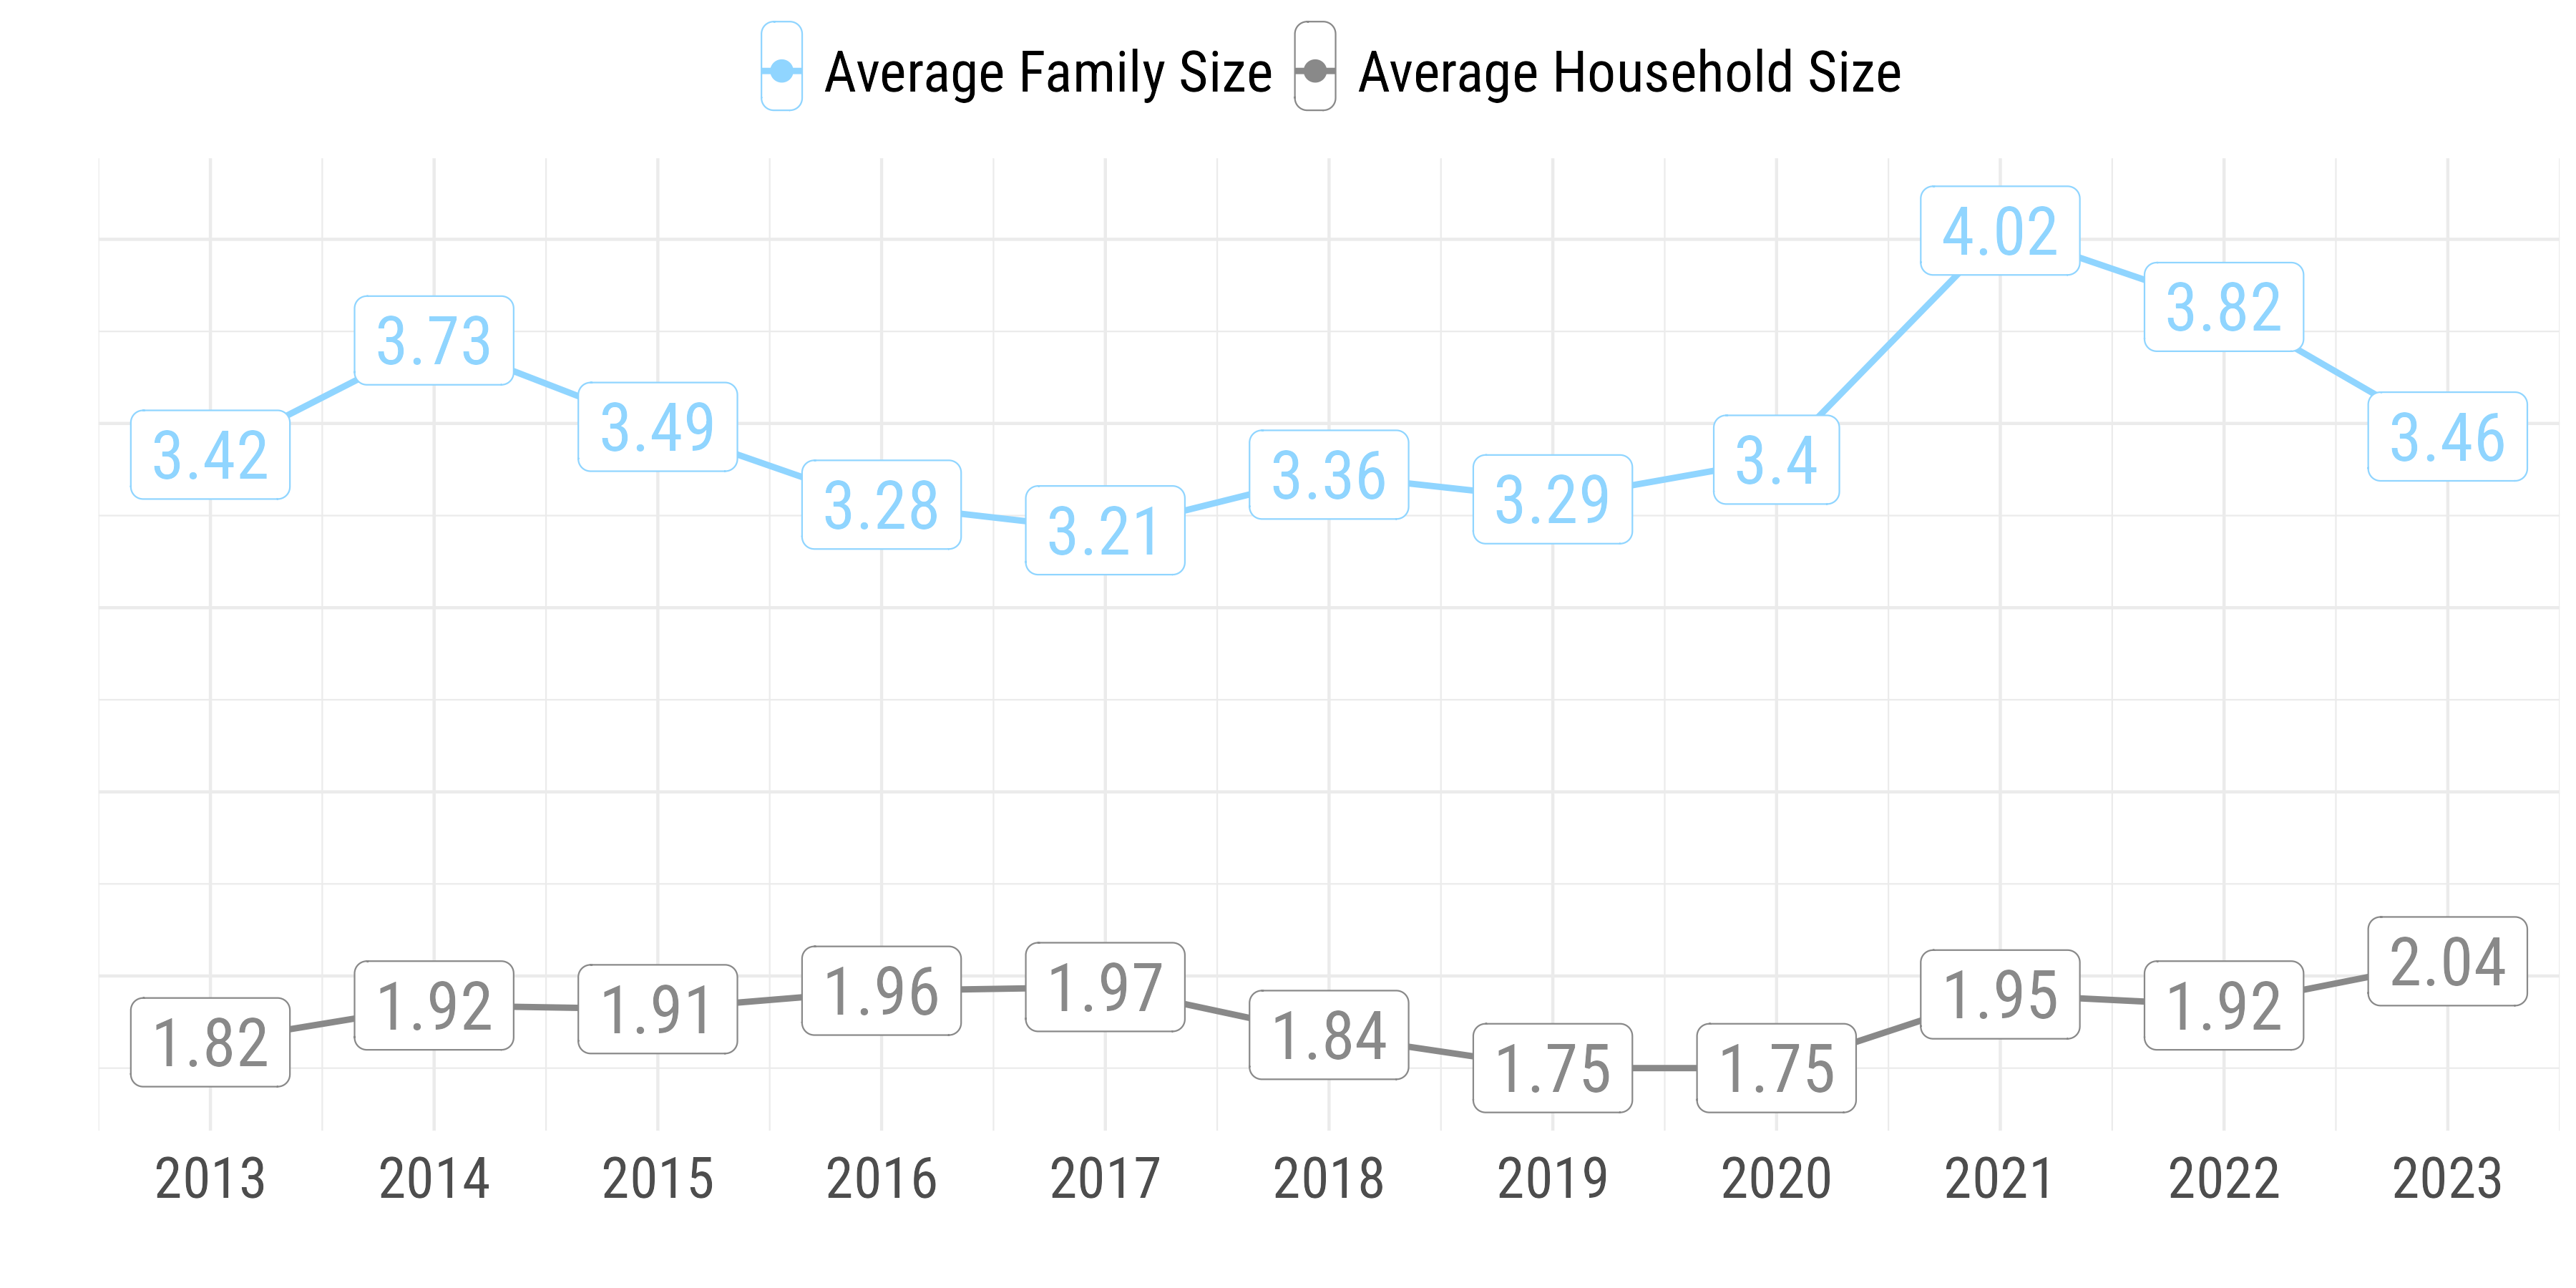
\includegraphics[width=\linewidth]{figures/household_size.png}
    \rule[-5pt]{\linewidth}{0.4pt}
    \floatnote{Data come from the \href{https://www.census.gov/programs-surveys/acs.html}{2013 through 2023 American Community Survey Five-Year Estimates}.}
\end{framed}
\end{figure}

\pagebreak
\subsubsection*{Median Age}

\noindent Bloomfield's population has steadily aged. \textbf{Figure~\ref{fig:medianAge}} shows how, between 2017 and 2019, the median age in Bloomfield jumped more than five years, and has steadily remained at just below sixty ever since.

\begin{figure}[H]
\centering
\begin{framed}
    \caption{Median Age, 2013-2023}
    \label{fig:medianAge}
    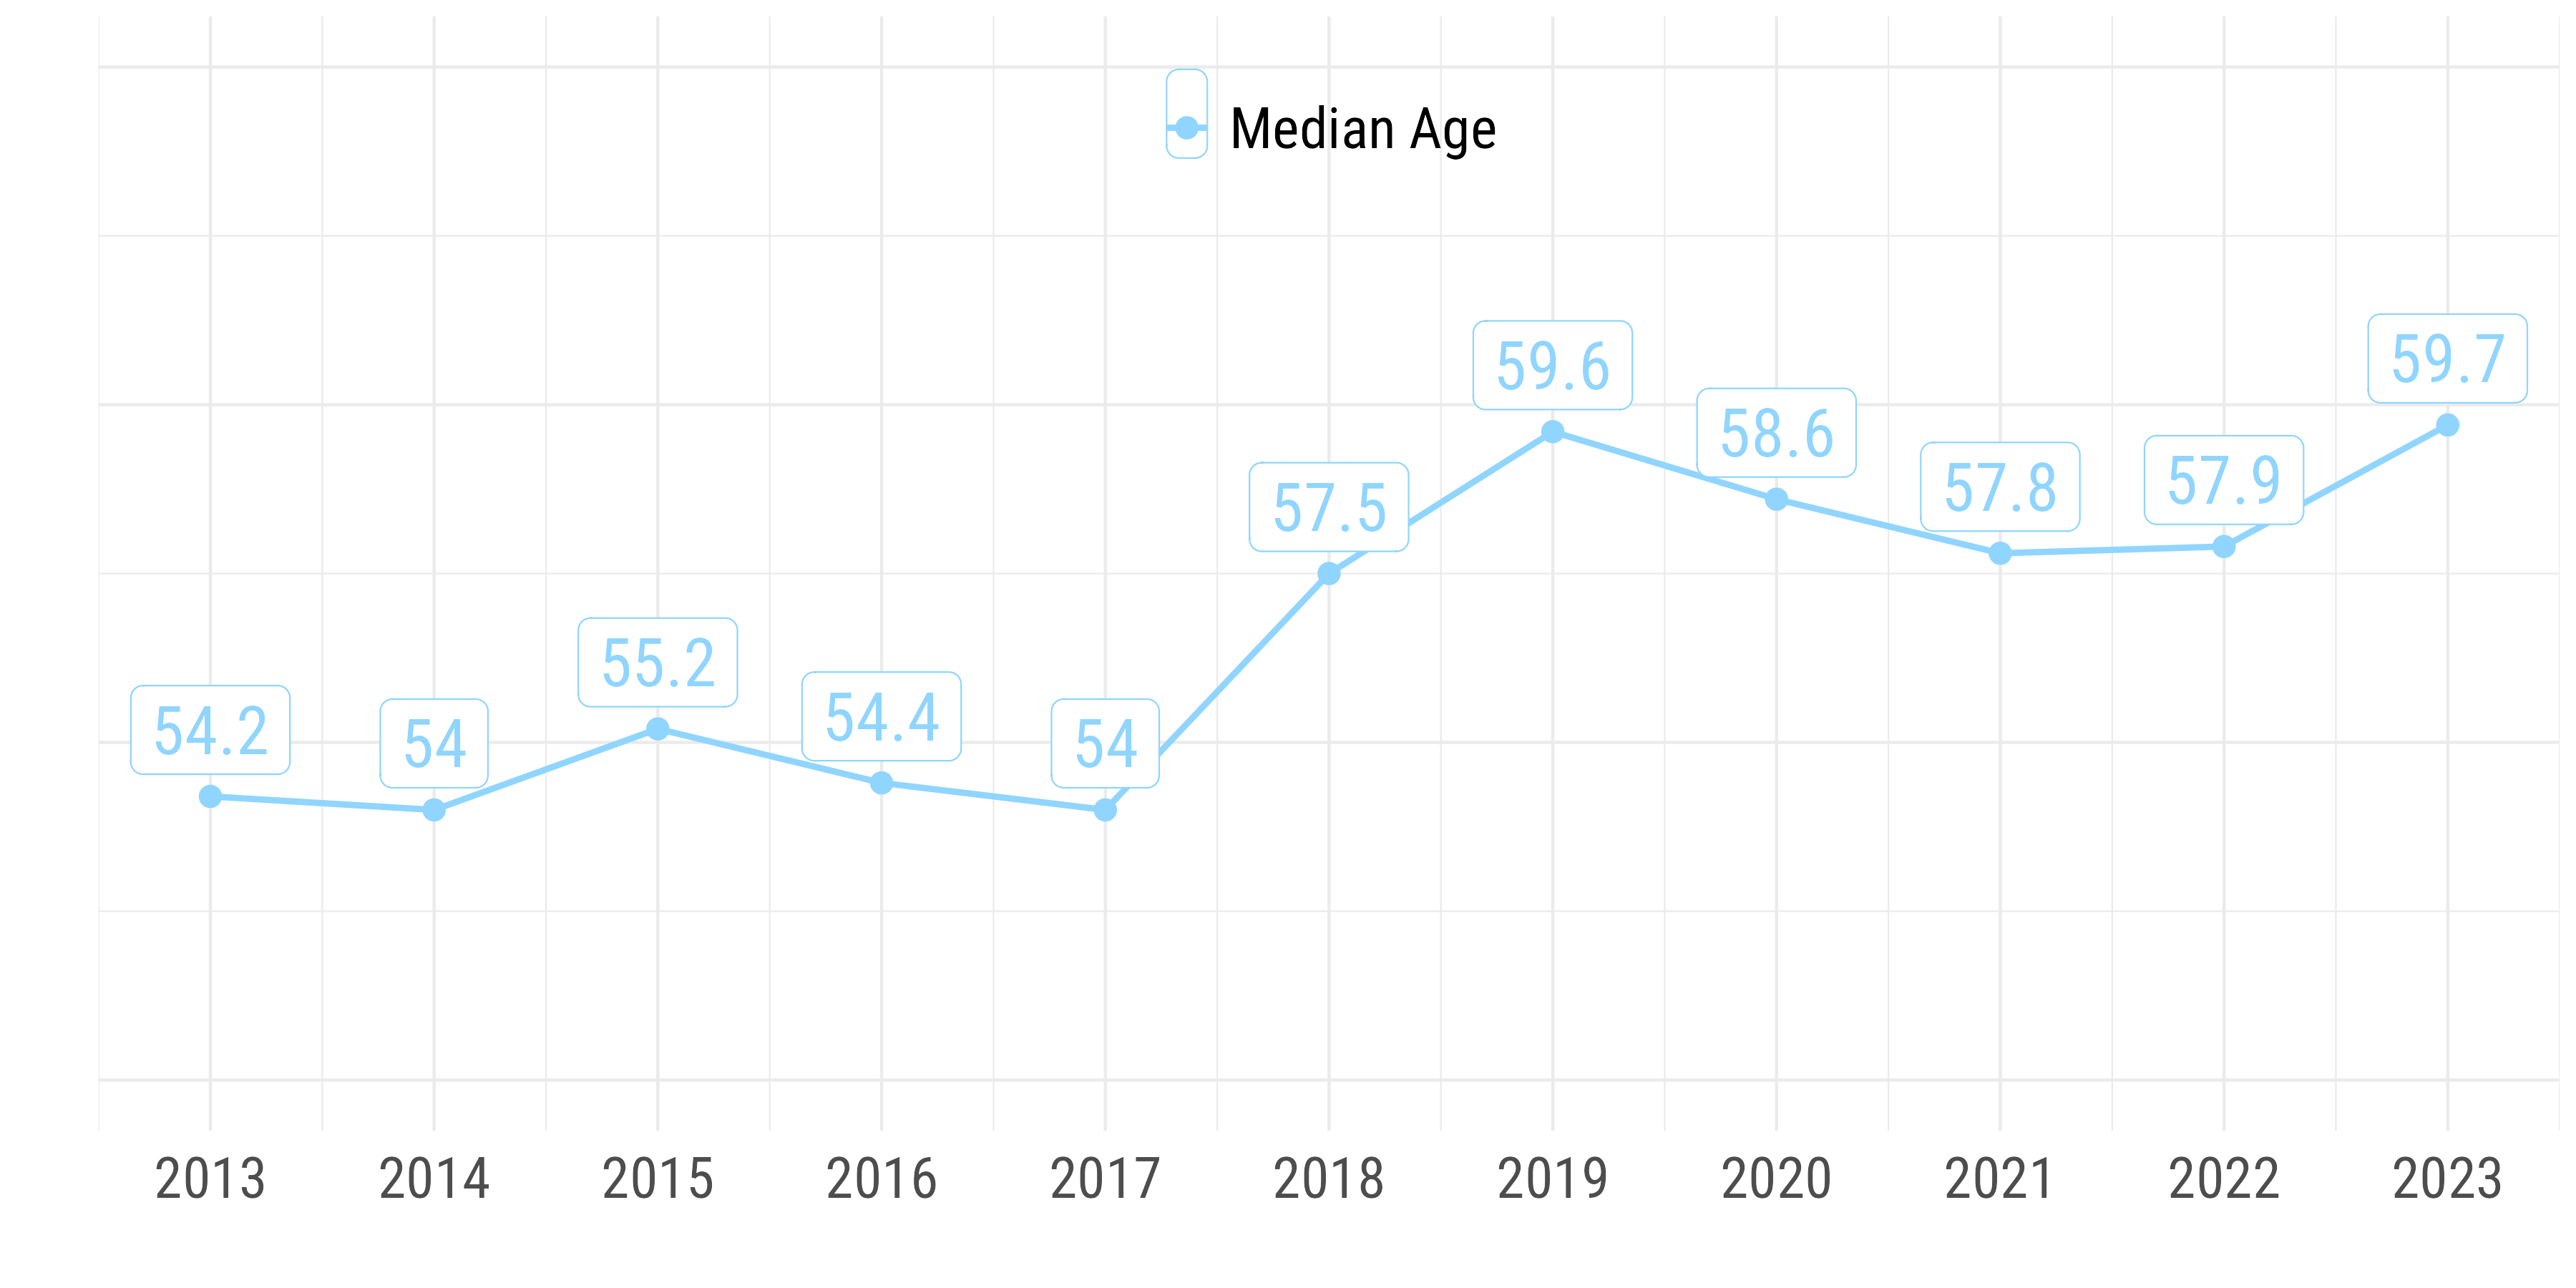
\includegraphics[width=\linewidth]{figures/median_age.png}
    \rule[-5pt]{\linewidth}{0.4pt}
    \floatnote{Data come from the \href{https://www.census.gov/programs-surveys/acs.html}{2013 through 2023 American Community Survey Five-Year Estimates}.}
\end{framed}
\end{figure}

\pagebreak
\subsubsection*{Housing Costs}

\noindent Overall, both incomes and costs of living have increased in Bloomfield over the last decade. \textbf{Figure~\ref{fig:housingCosts}} shows how, adjusting for inflation, each of median home values, median household incomes, and median gross rents in Bloomfield have slowly risen since 2013. However, much of that growth took place prior to 2020; over the last several years, these values have generally stagnated or even declined.

\begin{figure}[H]
\centering
\begin{framed}
    \caption{Housing Costs for Bloomfield, Nebraska}
    \label{fig:housingCosts}
    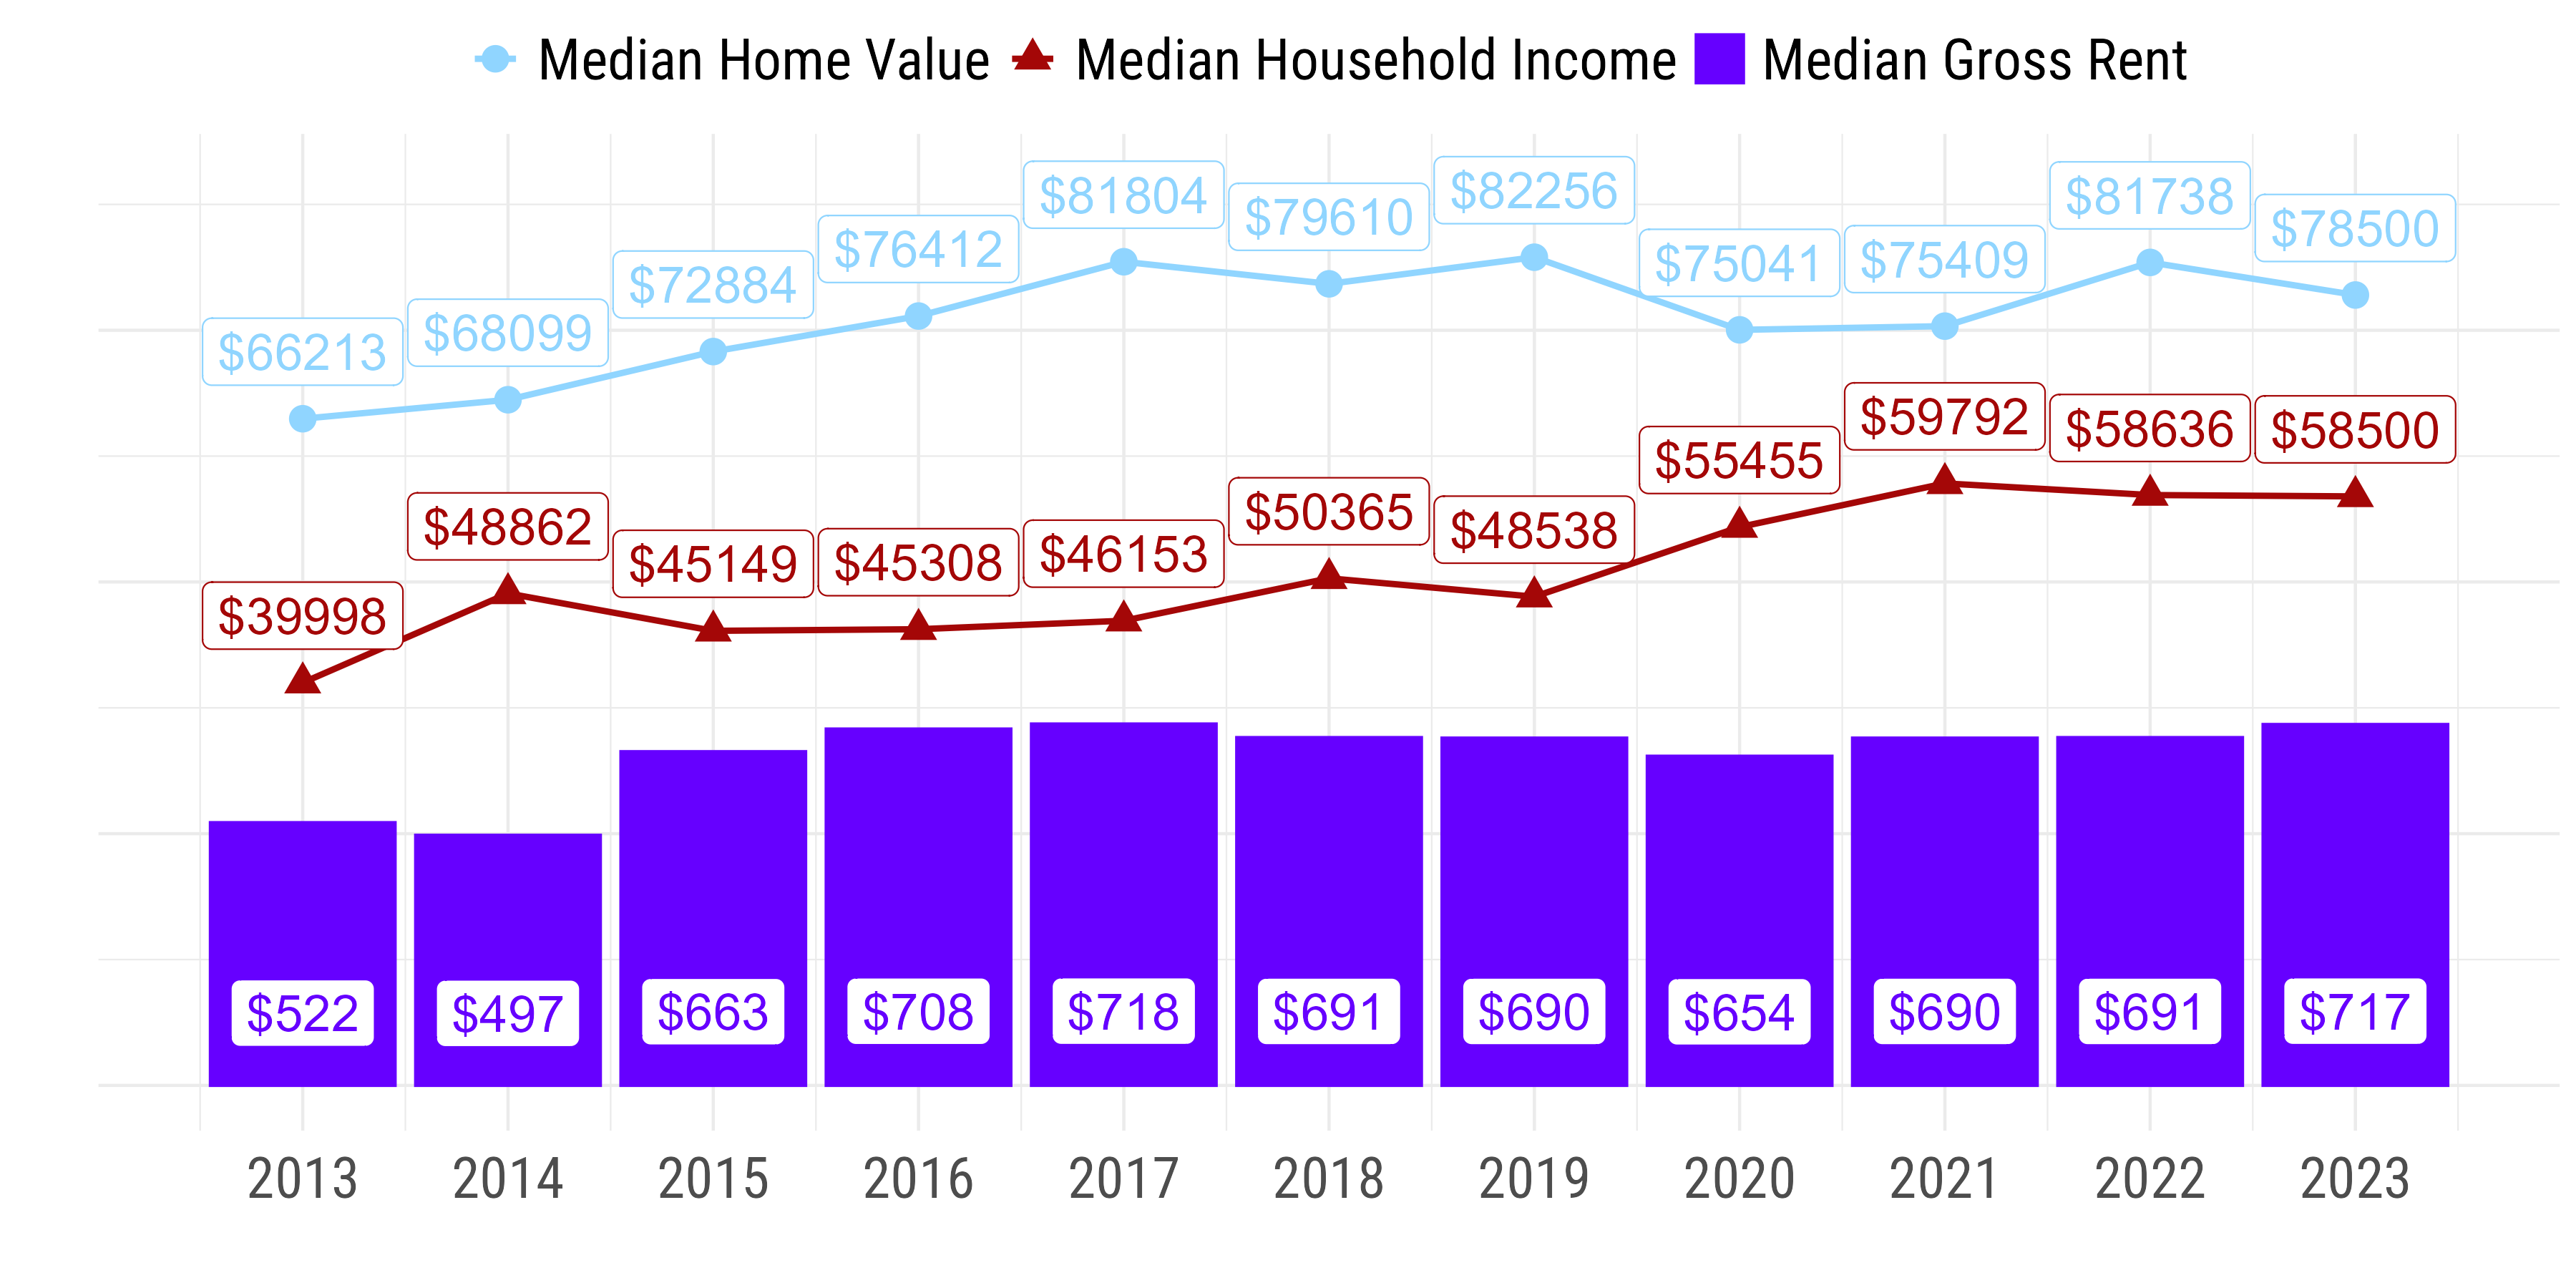
\includegraphics[width=\linewidth]{figures/housing_costs.png}
    \rule[-5pt]{\linewidth}{0.4pt}
    \floatnote{Data come from the \href{https://www.census.gov/programs-surveys/acs.html}{2013 through 2023 American Community Survey Five-Year Estimates}. Units are in 2023-adjusted real dollars.}
\end{framed}
\end{figure}

\pagebreak
\noindent Respondents to the community survey tend to be more affluent than the ACS would suggest. Fully two-thirds of respondents indicated that they have incomes above the Bloomfield median. Of that two-thirds, about half reported household incomes more than \$100,000. \textbf{Figure~\ref{fig:householdIncomes}} documents this distribution.

\begin{figure}[H]
\centering
\begin{framed}
    \caption{Household Incomes for Bloomfield, Nebraska}
    \label{fig:householdIncomes}
    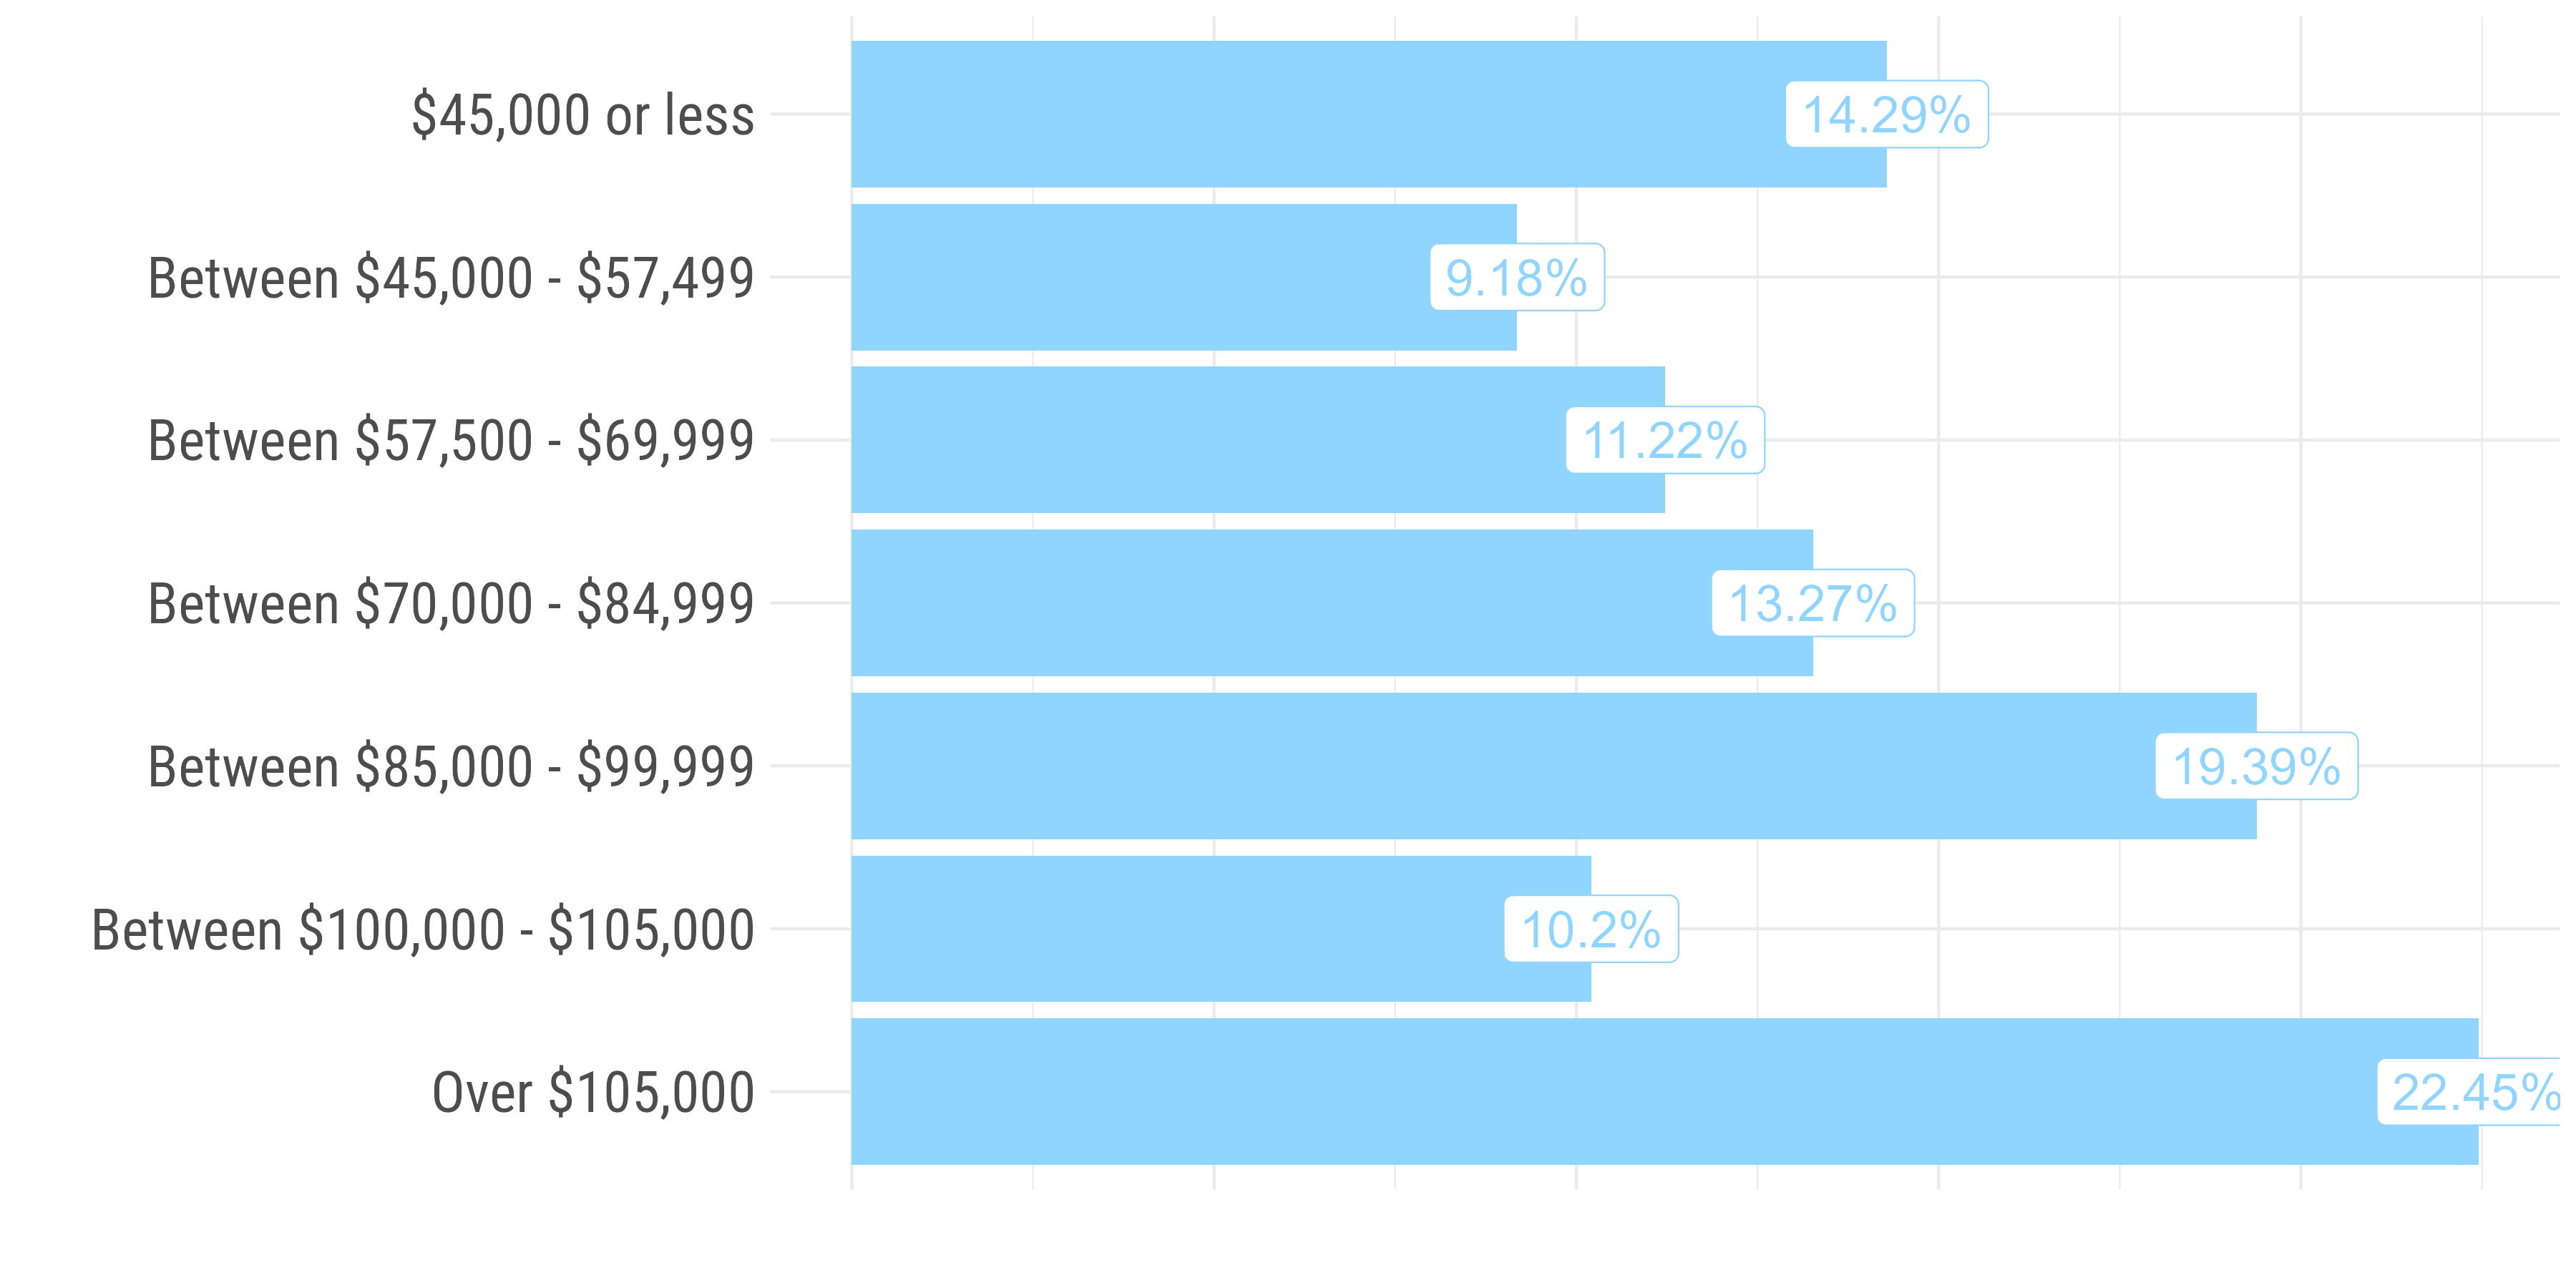
\includegraphics[width=\linewidth]{figures/survey_respondent_incomes.png}
    \rule[-5pt]{\linewidth}{0.4pt}
    % \floatnote{Data come from the \href{https://www.census.gov/programs-surveys/acs.html}{2013 through 2023 American Community Survey Five-Year Estimates}. Units are in 2023-adjusted real dollars.}
\end{framed}
\end{figure}

\pagebreak
\noindent Despite this, survey respondents experience housing situations close to the \href{https://www.hudexchange.info/programs/home/home-income-limits}{Department of Housing and Urban Development's (HUD) guidelines} that affordable housing costs no more than thirty percent of one's income. Per \textbf{Figure~\ref{fig:housingCostsSurvey}}, about seventy percent of Bloomfield respondents are at or above the thirty percent guideline.

\begin{figure}[H]
\centering
\begin{framed}
    \caption{Housing Costs for Bloomfield, Nebraska}
    \label{fig:housingCostsSurvey}
    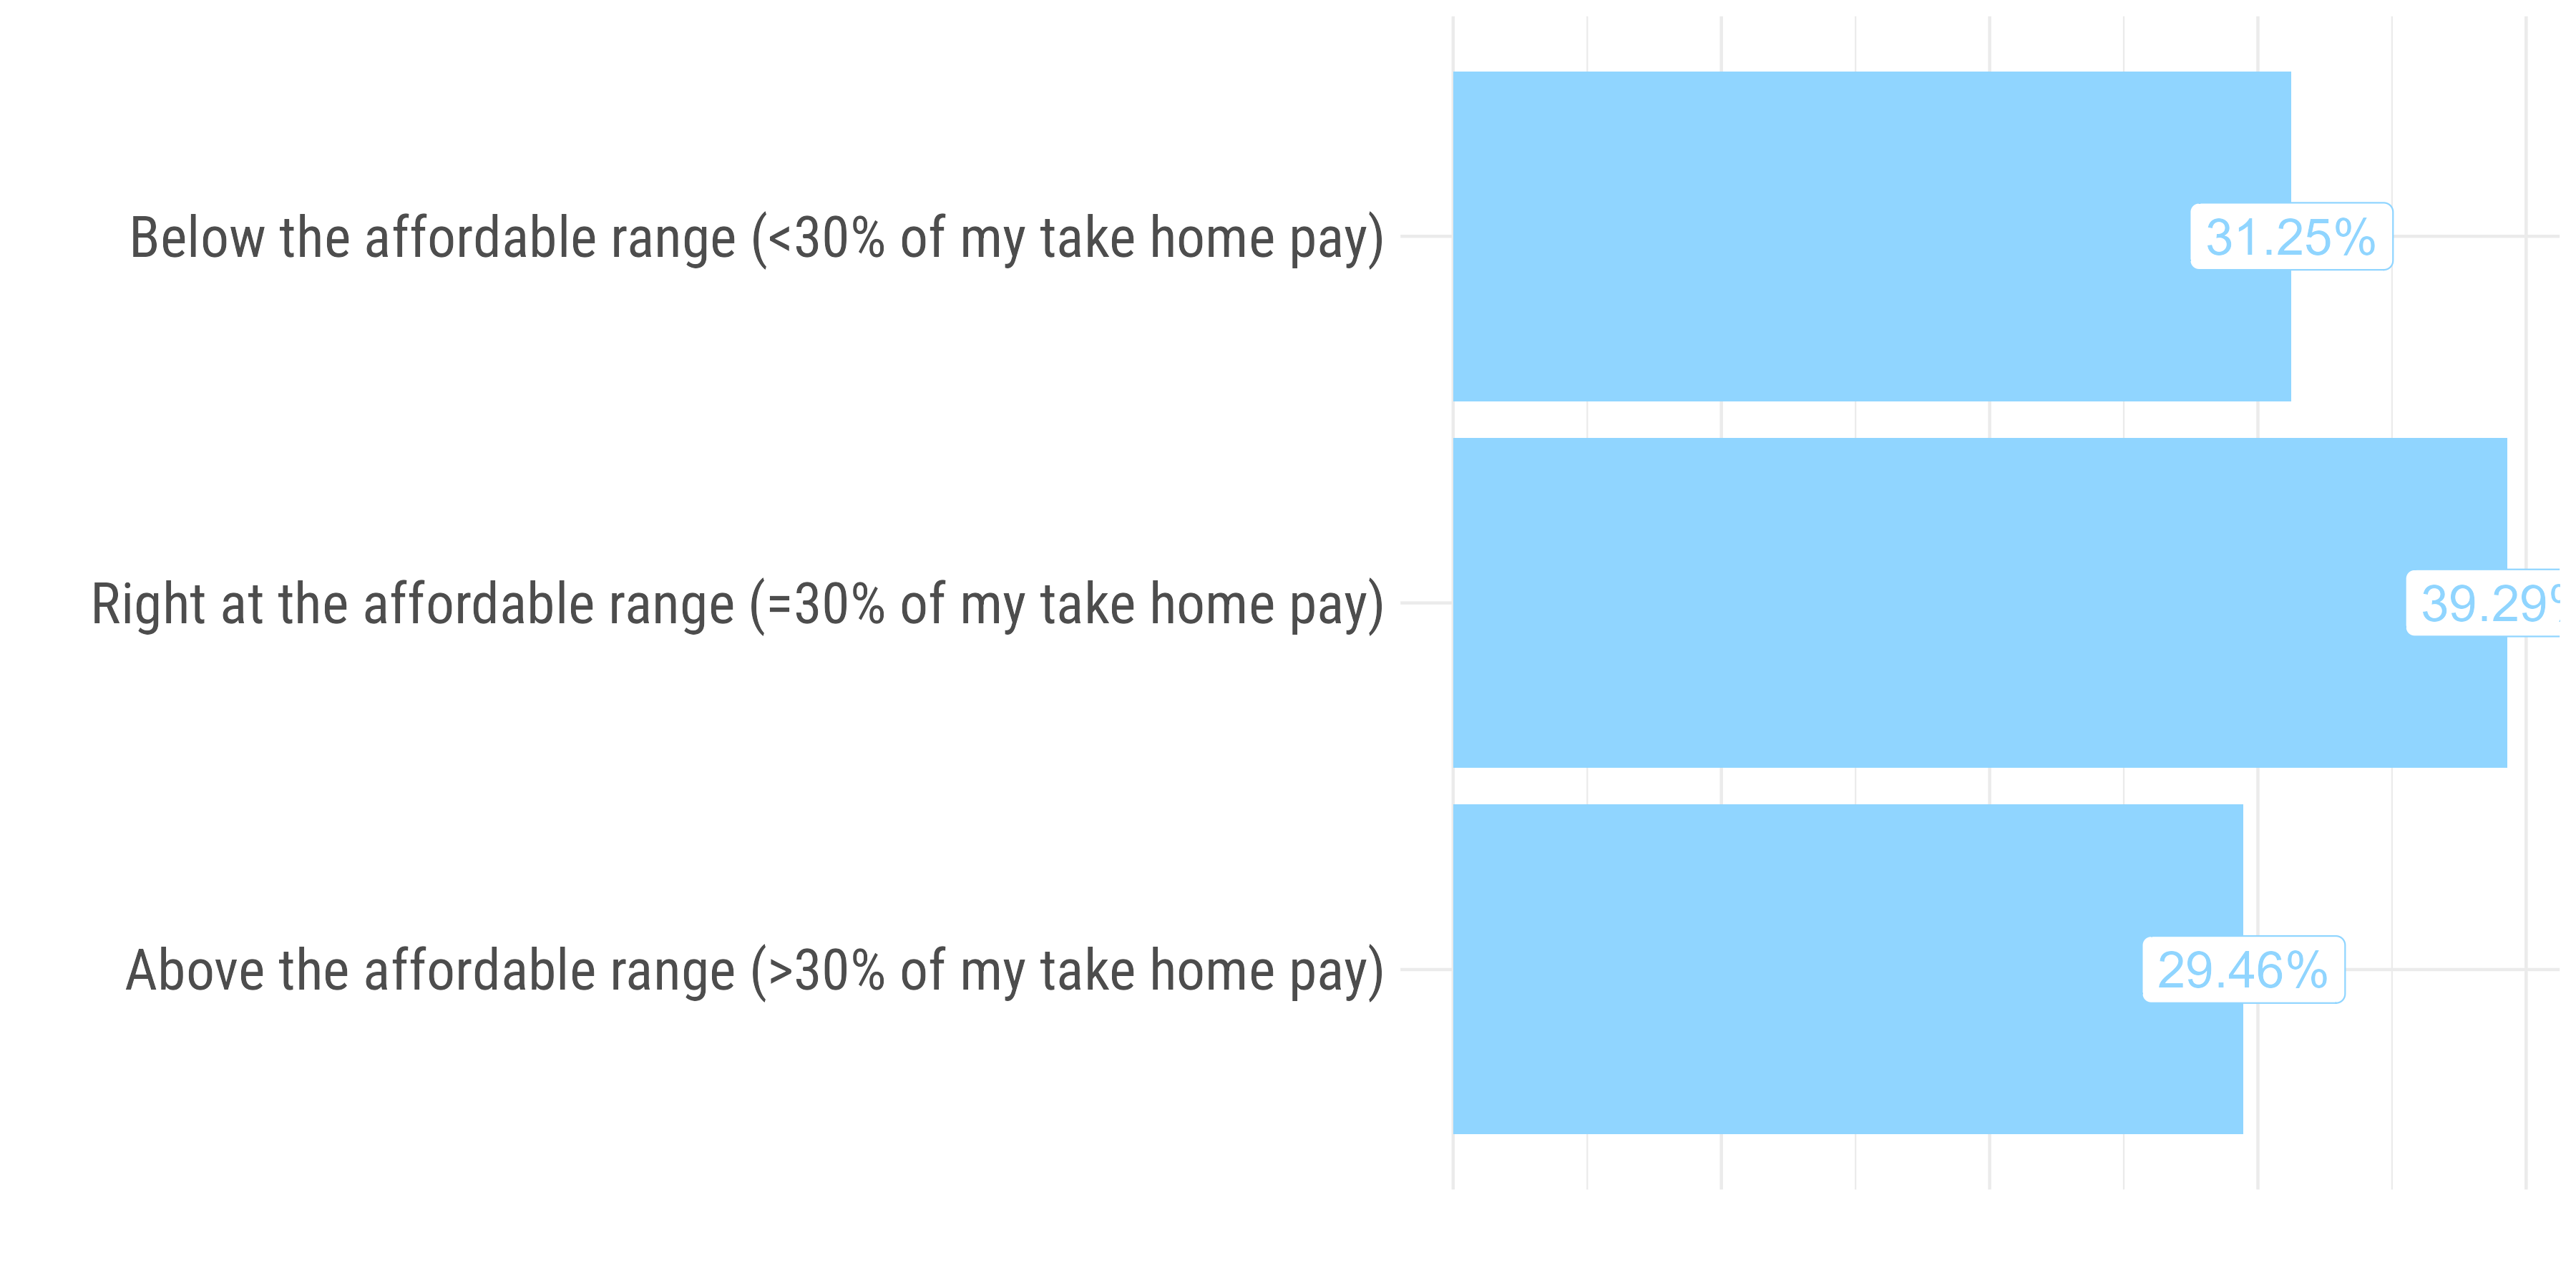
\includegraphics[width=\linewidth]{figures/survey_respondent_housing_costs.png}
    \rule[-5pt]{\linewidth}{0.4pt}
    % \floatnote{Data come from the \href{https://www.census.gov/programs-surveys/acs.html}{2013 through 2023 American Community Survey Five-Year Estimates}. Units are in 2023-adjusted real dollars.}
\end{framed}
\end{figure}

\pagebreak
\subsection*{Key Takeaways}
\pagebreak
\section{Commercial and Business Assessment}

\subsection{Condition of Commercial Structures}

\noindent \hl{[redo assessor map with commerical-listed parcels]}

\subsection{Business Establishments}

\noindent Over the last five years, the number of business establishments in Knox County has changed very little. \textbf{Figure~\ref{fig:bizEstablishments}} shows that the total number of businesses has decreased by just two during this time. All of the business loss is driven by fewer government establishments, while the number of private sector businesses has increased.

\begin{figure}[ht!]
\centering
\begin{framed}
    \caption{Business Establishments in Knox County, Nebraska}
    \label{fig:bizEstablishments}
    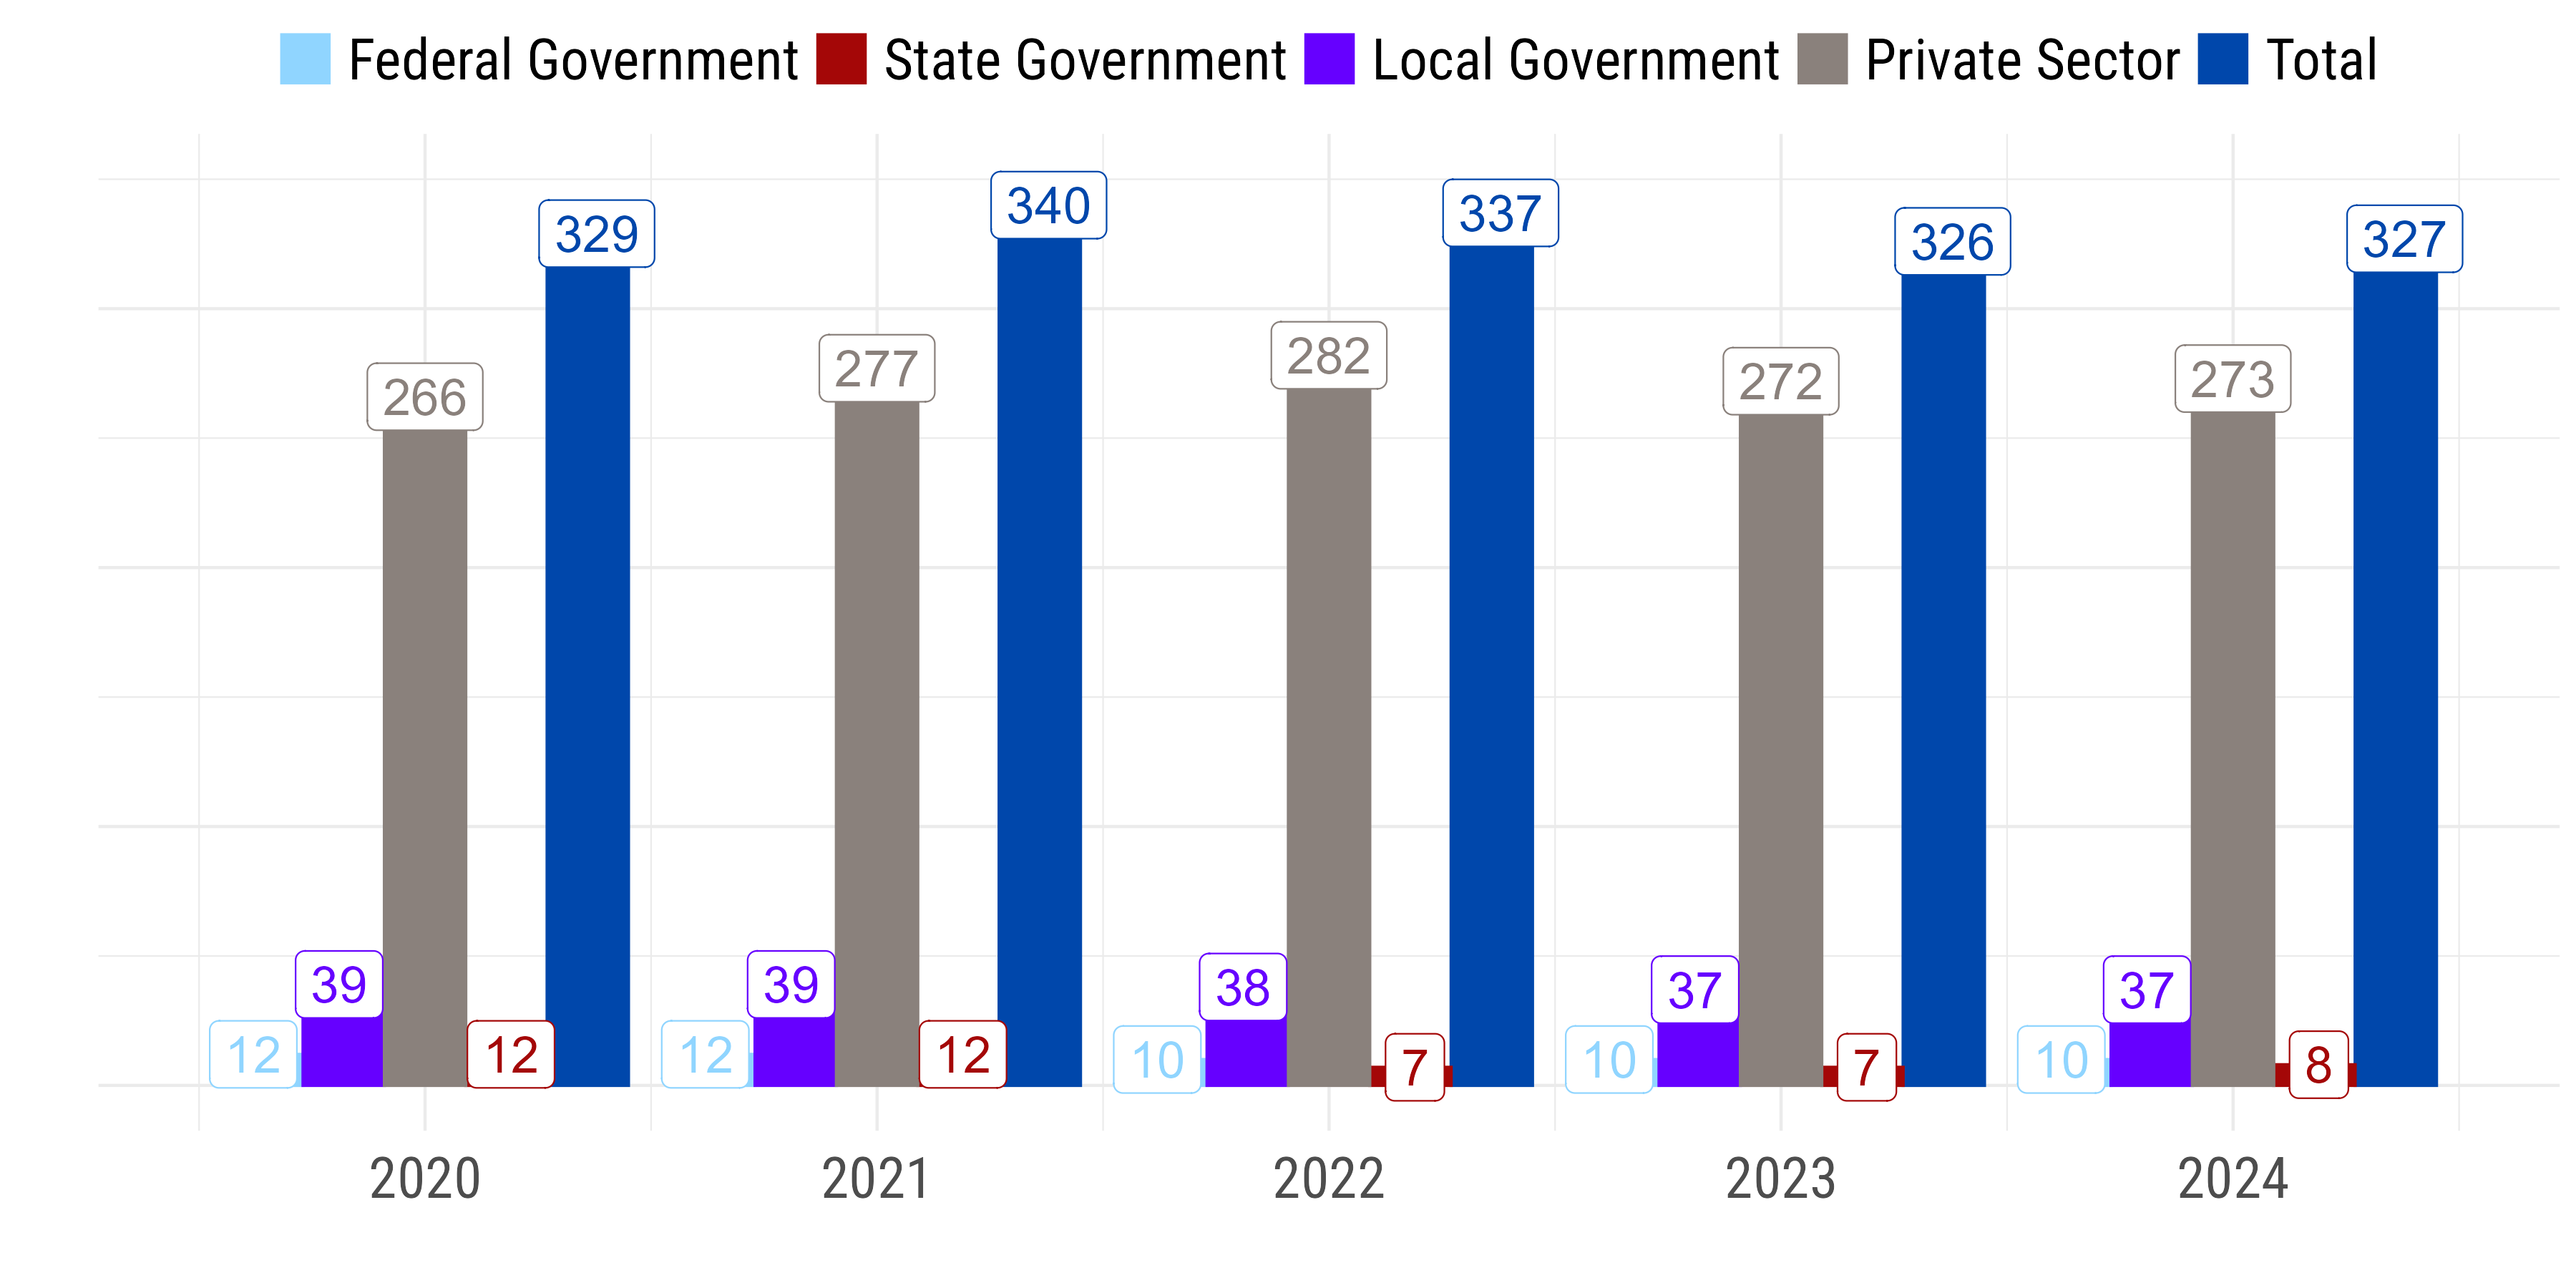
\includegraphics[width=\linewidth]{figures/knox_county_employers.png}
    \rule[-5pt]{\linewidth}{0.4pt}
    \floatnote{Data come from the \href{https://www.bls.gov/cew/}{Bureau of Labor Statistics Quarterly Census of Employment and Wages}.}
\end{framed}
\end{figure}


% \subsubsection{Auto Services and Freight Carriers}
% \subsubsection{Banking and Insurance}
% \subsubsection{Churches and Civic Organizations}
% \subsubsection{Communications}
% \subsubsection{Construction, Electricity, and Welding}
% \subsubsection{Grocery}
% \subsubsection{Hair Salon and Barbershop}
% \subsubsection{Lodging}
% \subsubsection{Medical and Pharmaceutical Services}
% \subsubsection{Nursing and Assisted Living}
% \subsubsection{Professional Services}
% \subsubsection{Residential Services}
% \subsubsection{Restaurants, Liquor, and Hospitality}
% \subsubsection{Retail}

\subsection{Labor, Wages, and Earnings}

\noindent \hl{[redo previous fig with wage and employee data]}

\subsection{Economic Activity}

\noindent Overall economic activity in Bloomfield and other comparable cities has varied over the last decade. \textbf{Figure~\ref{fig:netTaxableSales}} shows how, adjusting for inflation, the cumulative volume of taxable sales in Bloomfield has increased by about nine percent. In nearby Creighton, it has decreased by about eight percent. And in Crofton, excluding an outlier year in 2014, the volume of net taxable sales has decreased by about two percent.

\begin{figure}[H]
\centering
\begin{framed}
    \caption{Net Taxable Sales in Knox County, Nebraska}
    \label{fig:netTaxableSales}
    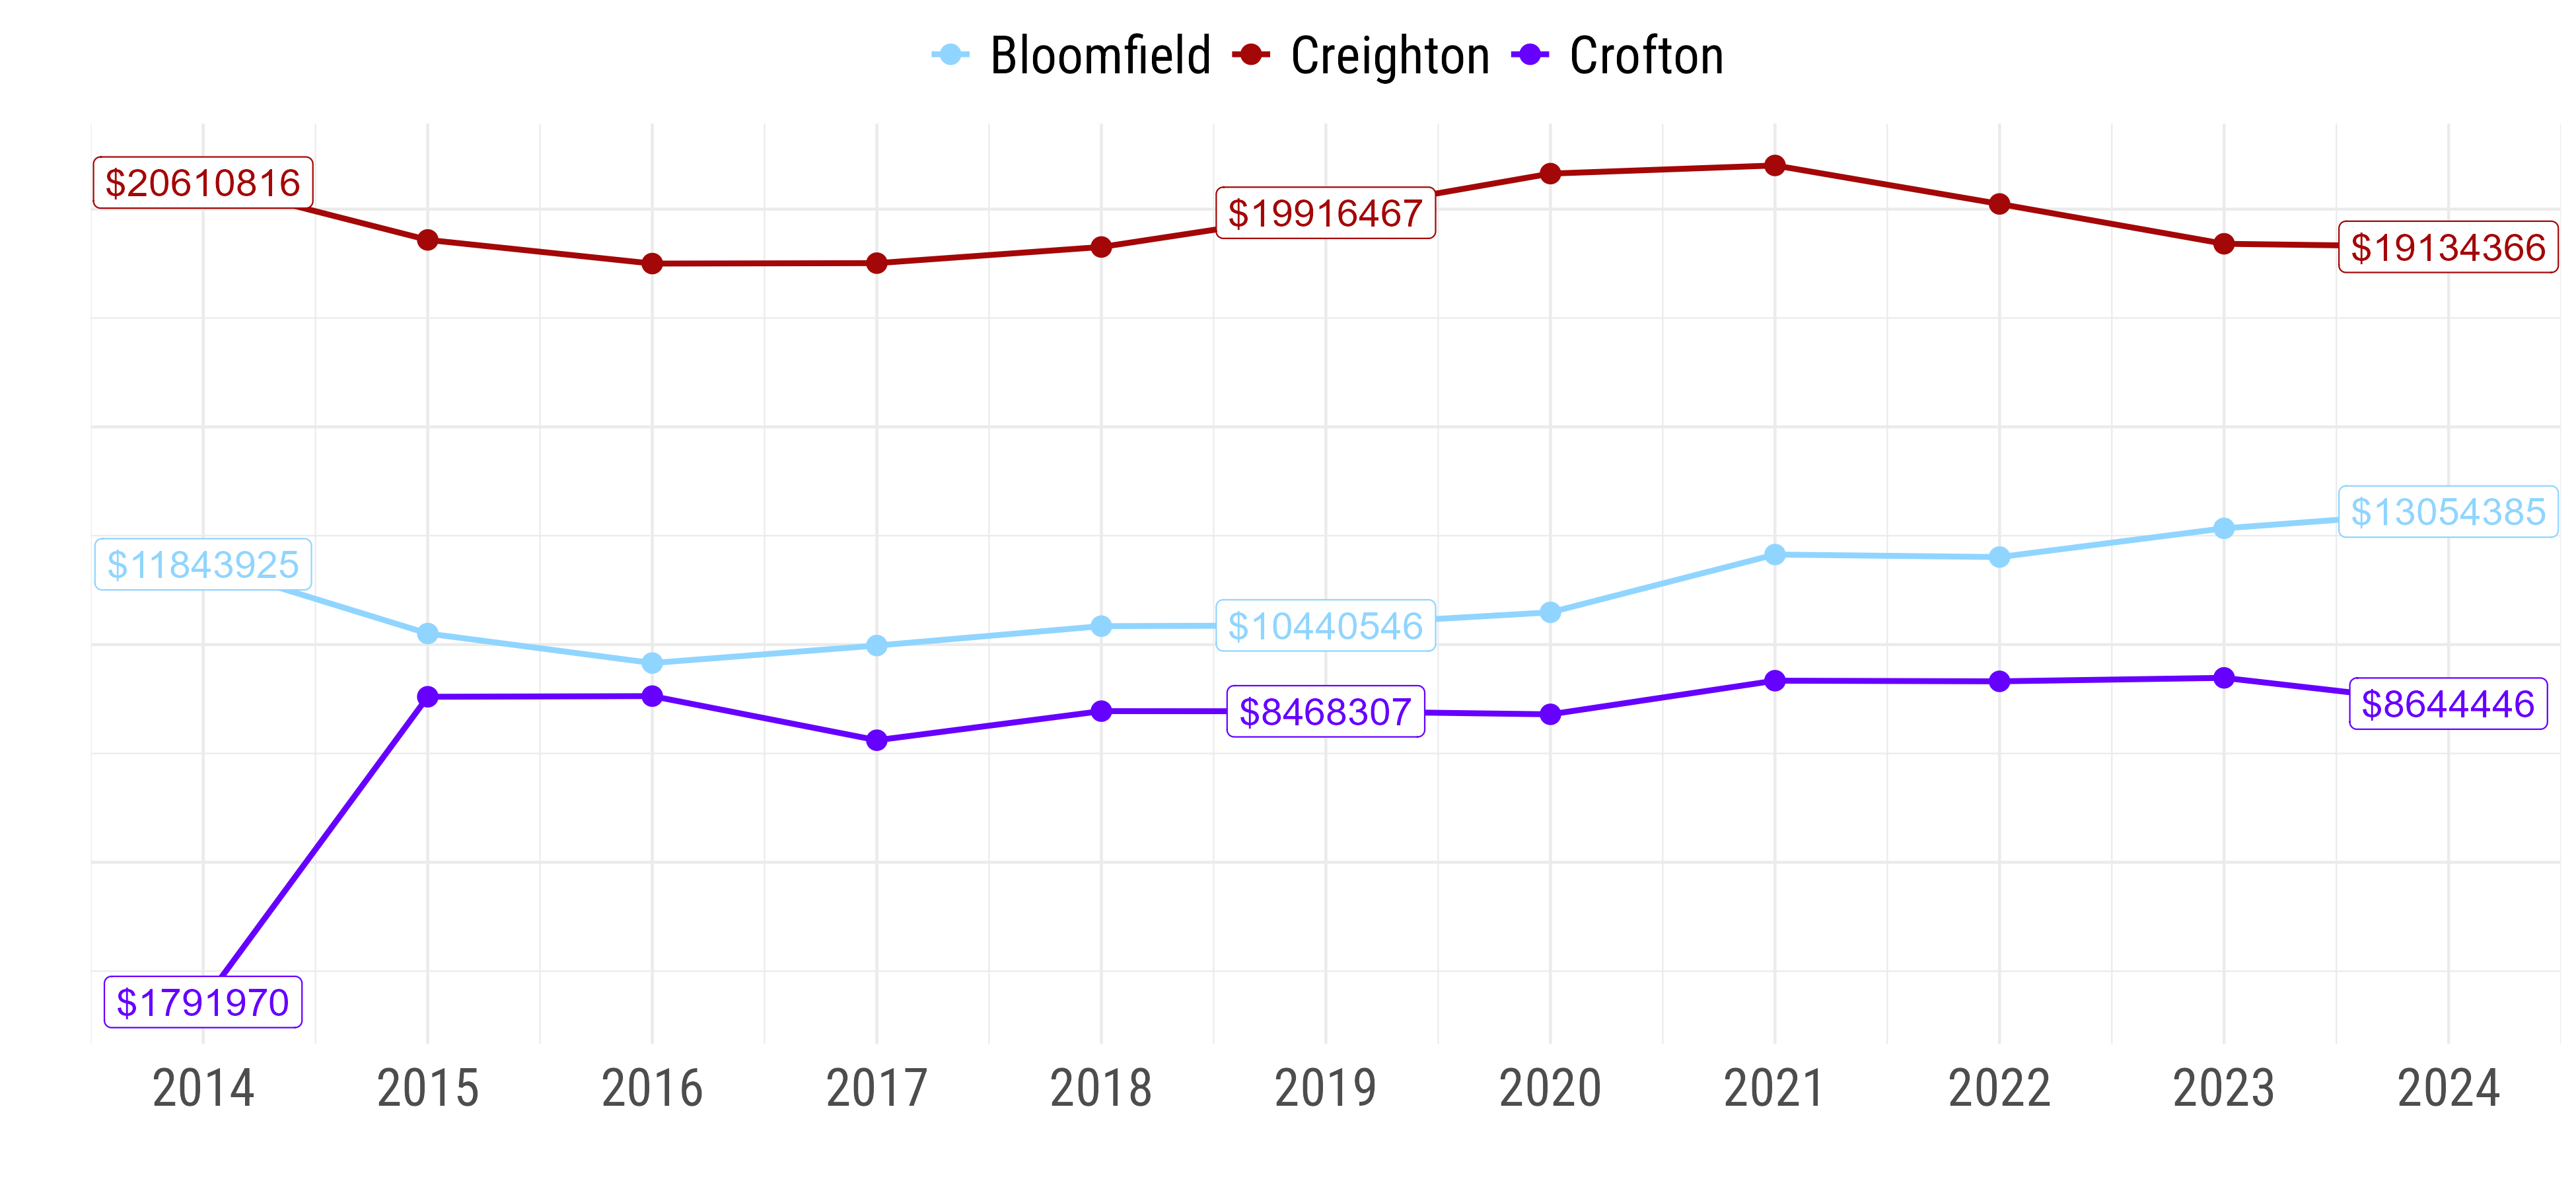
\includegraphics[width=\linewidth]{figures/net_taxable_sales.png}
    \rule[-5pt]{\linewidth}{0.4pt}
    \floatnote{Data come from the \href{https://revenue.nebraska.gov/research/statistics/sales-tax-data}{Nebraska Department of Revenue}. Units are in 2024-adjusted real dollars.}
\end{framed}
\end{figure}

\pagebreak
\subsection*{Key Takeaways}
\pagebreak
\section{Transportation Routes}

\noindent \href{https://nebraskalegislature.gov/laws/statutes.php?statute=19-903}{NRS \S 19-903(2)} requires a comprehensive development to include:

\begin{quote}
    The general location, character, and extent of existing and proposed major roads, streets, and highways, and air and other transportation routes and facilities.
\end{quote}

% \subsection{Surface Transportation Routes}

\noindent Bloomfield has two major roads: Broadway Street traverses north and south, while Highway 84 traverses east and west. Residents have differing assessments of the condition of these streets (refer to \textbf{Figure~\ref{fig:scoreStreets}}): the quality of Broadway Street is in rough shape, but Highway 84 is generally fine.

\begin{figure}[H]
\centering
\begin{framed}
    \caption{Condition of Specific Streets in Bloomfield}
    \label{fig:scoreStreets}
    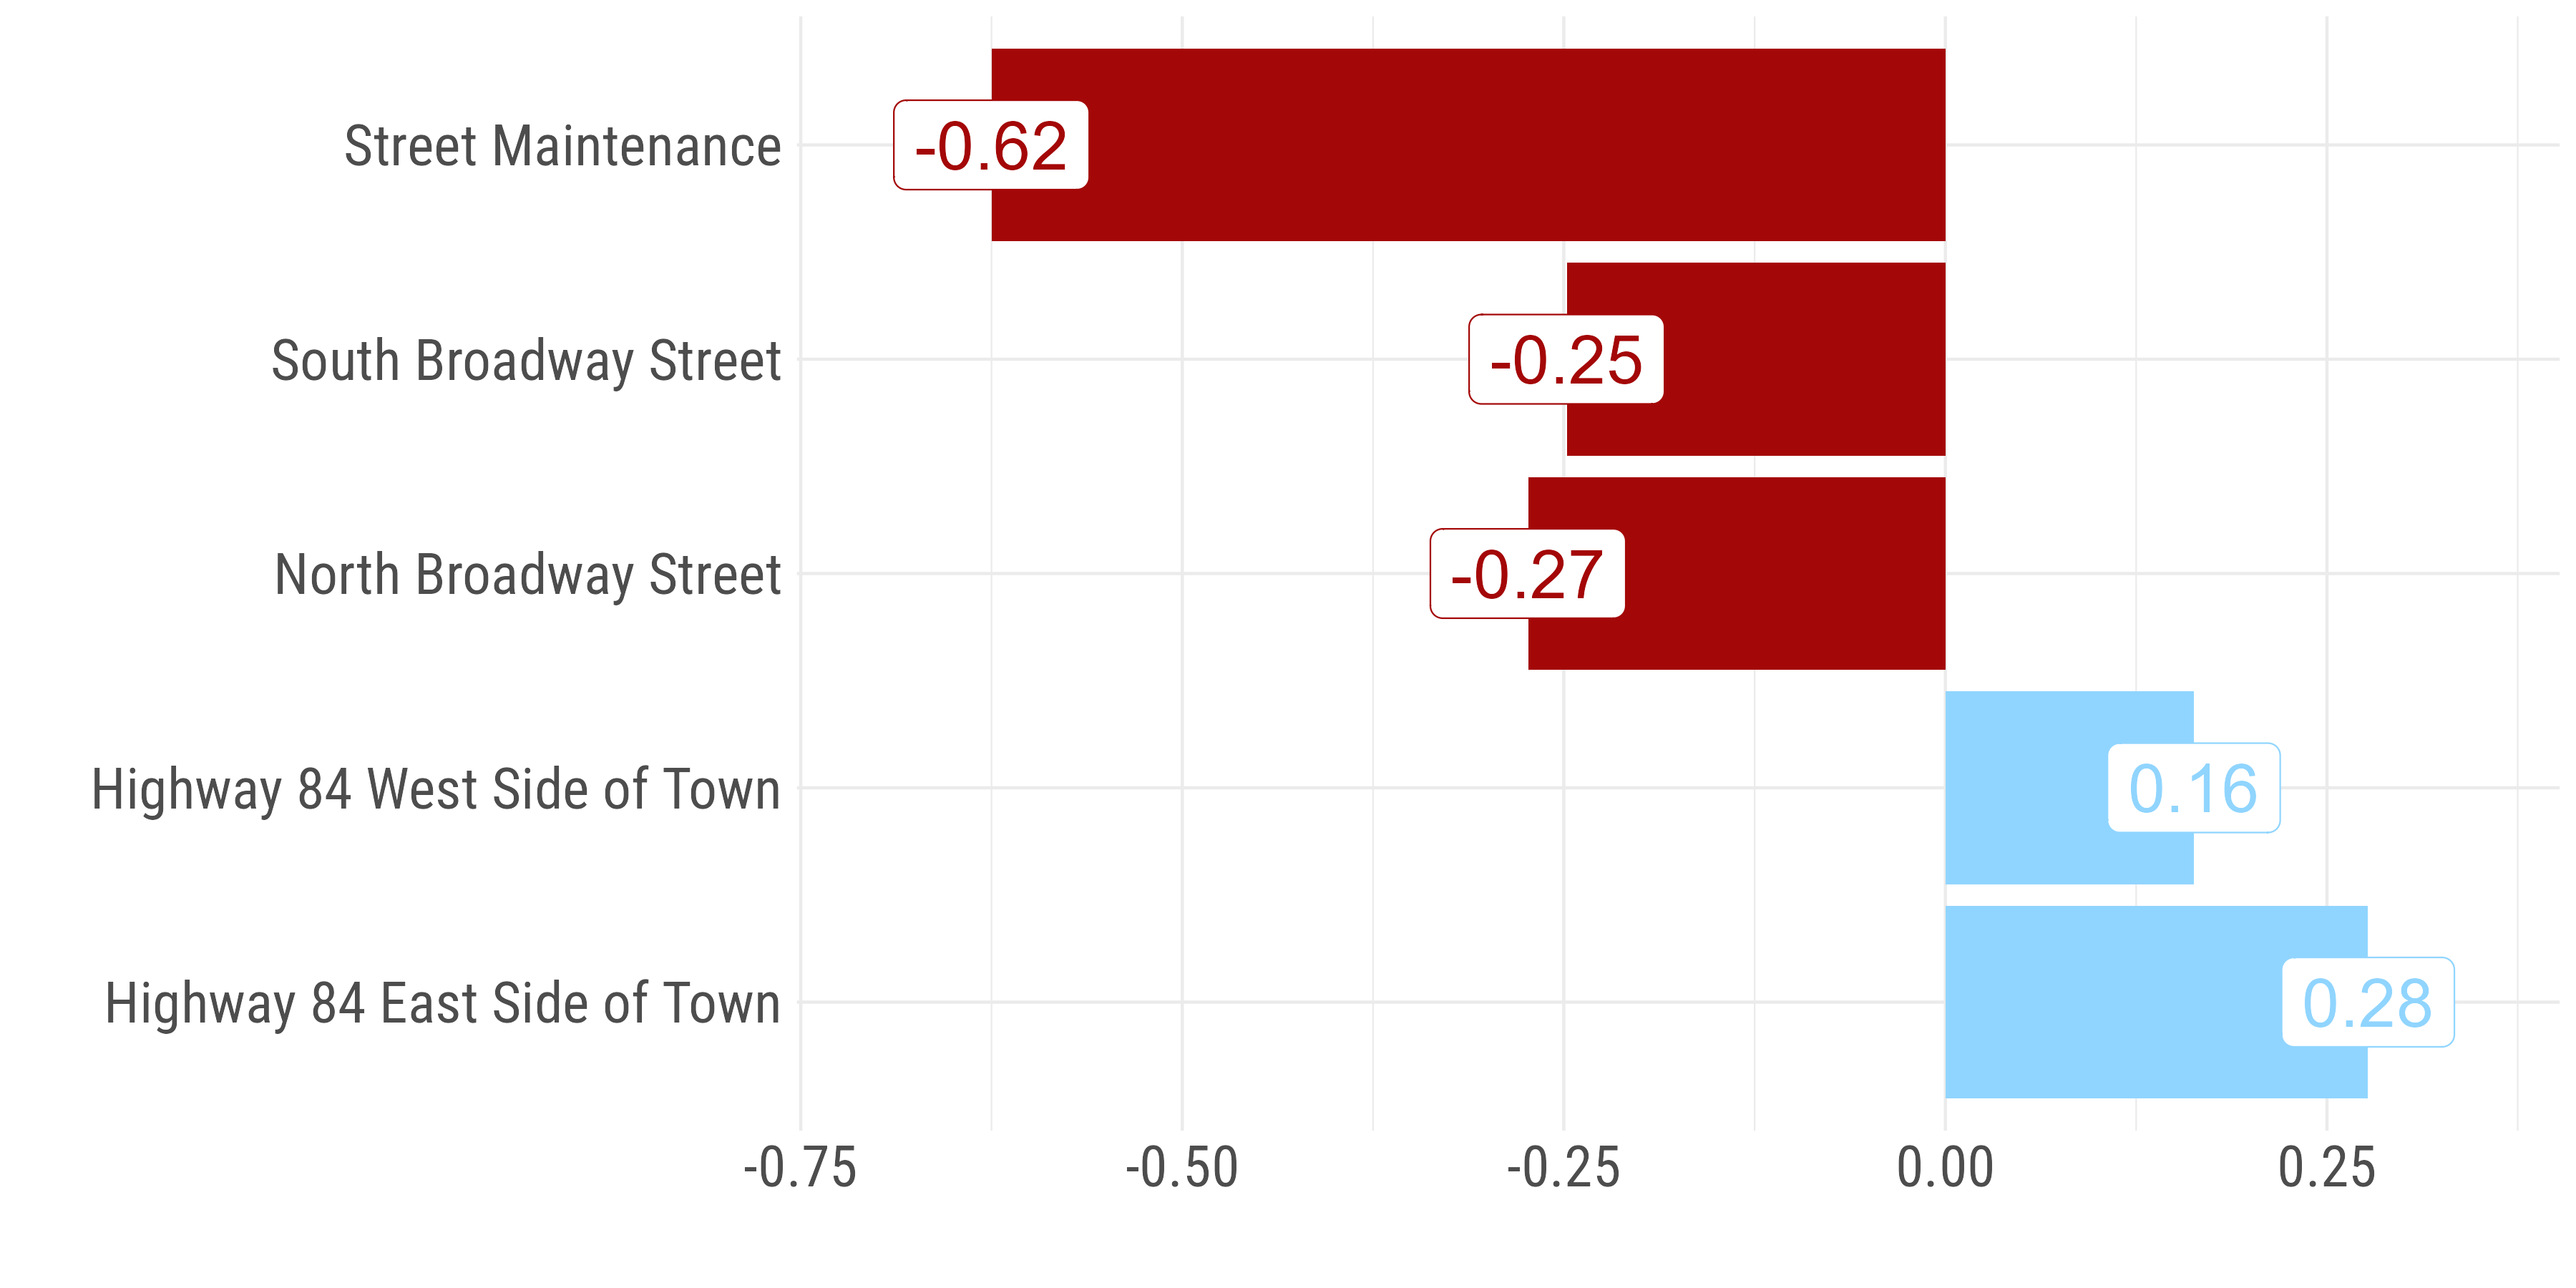
\includegraphics[width = \linewidth]{figures/score_streets.png}
\end{framed}
\end{figure}

\pagebreak
\noindent Moreover, community assessment of streets and sidewalks throughout Bloomfield is generally negative, as \textbf{Figure~\ref{fig:scoreStreetsGeneral}} shows.

\begin{figure}[H]
\centering
\begin{framed}
    \caption{Condition of General Streets and Sidewalks}
    \label{fig:scoreStreetsGeneral}
    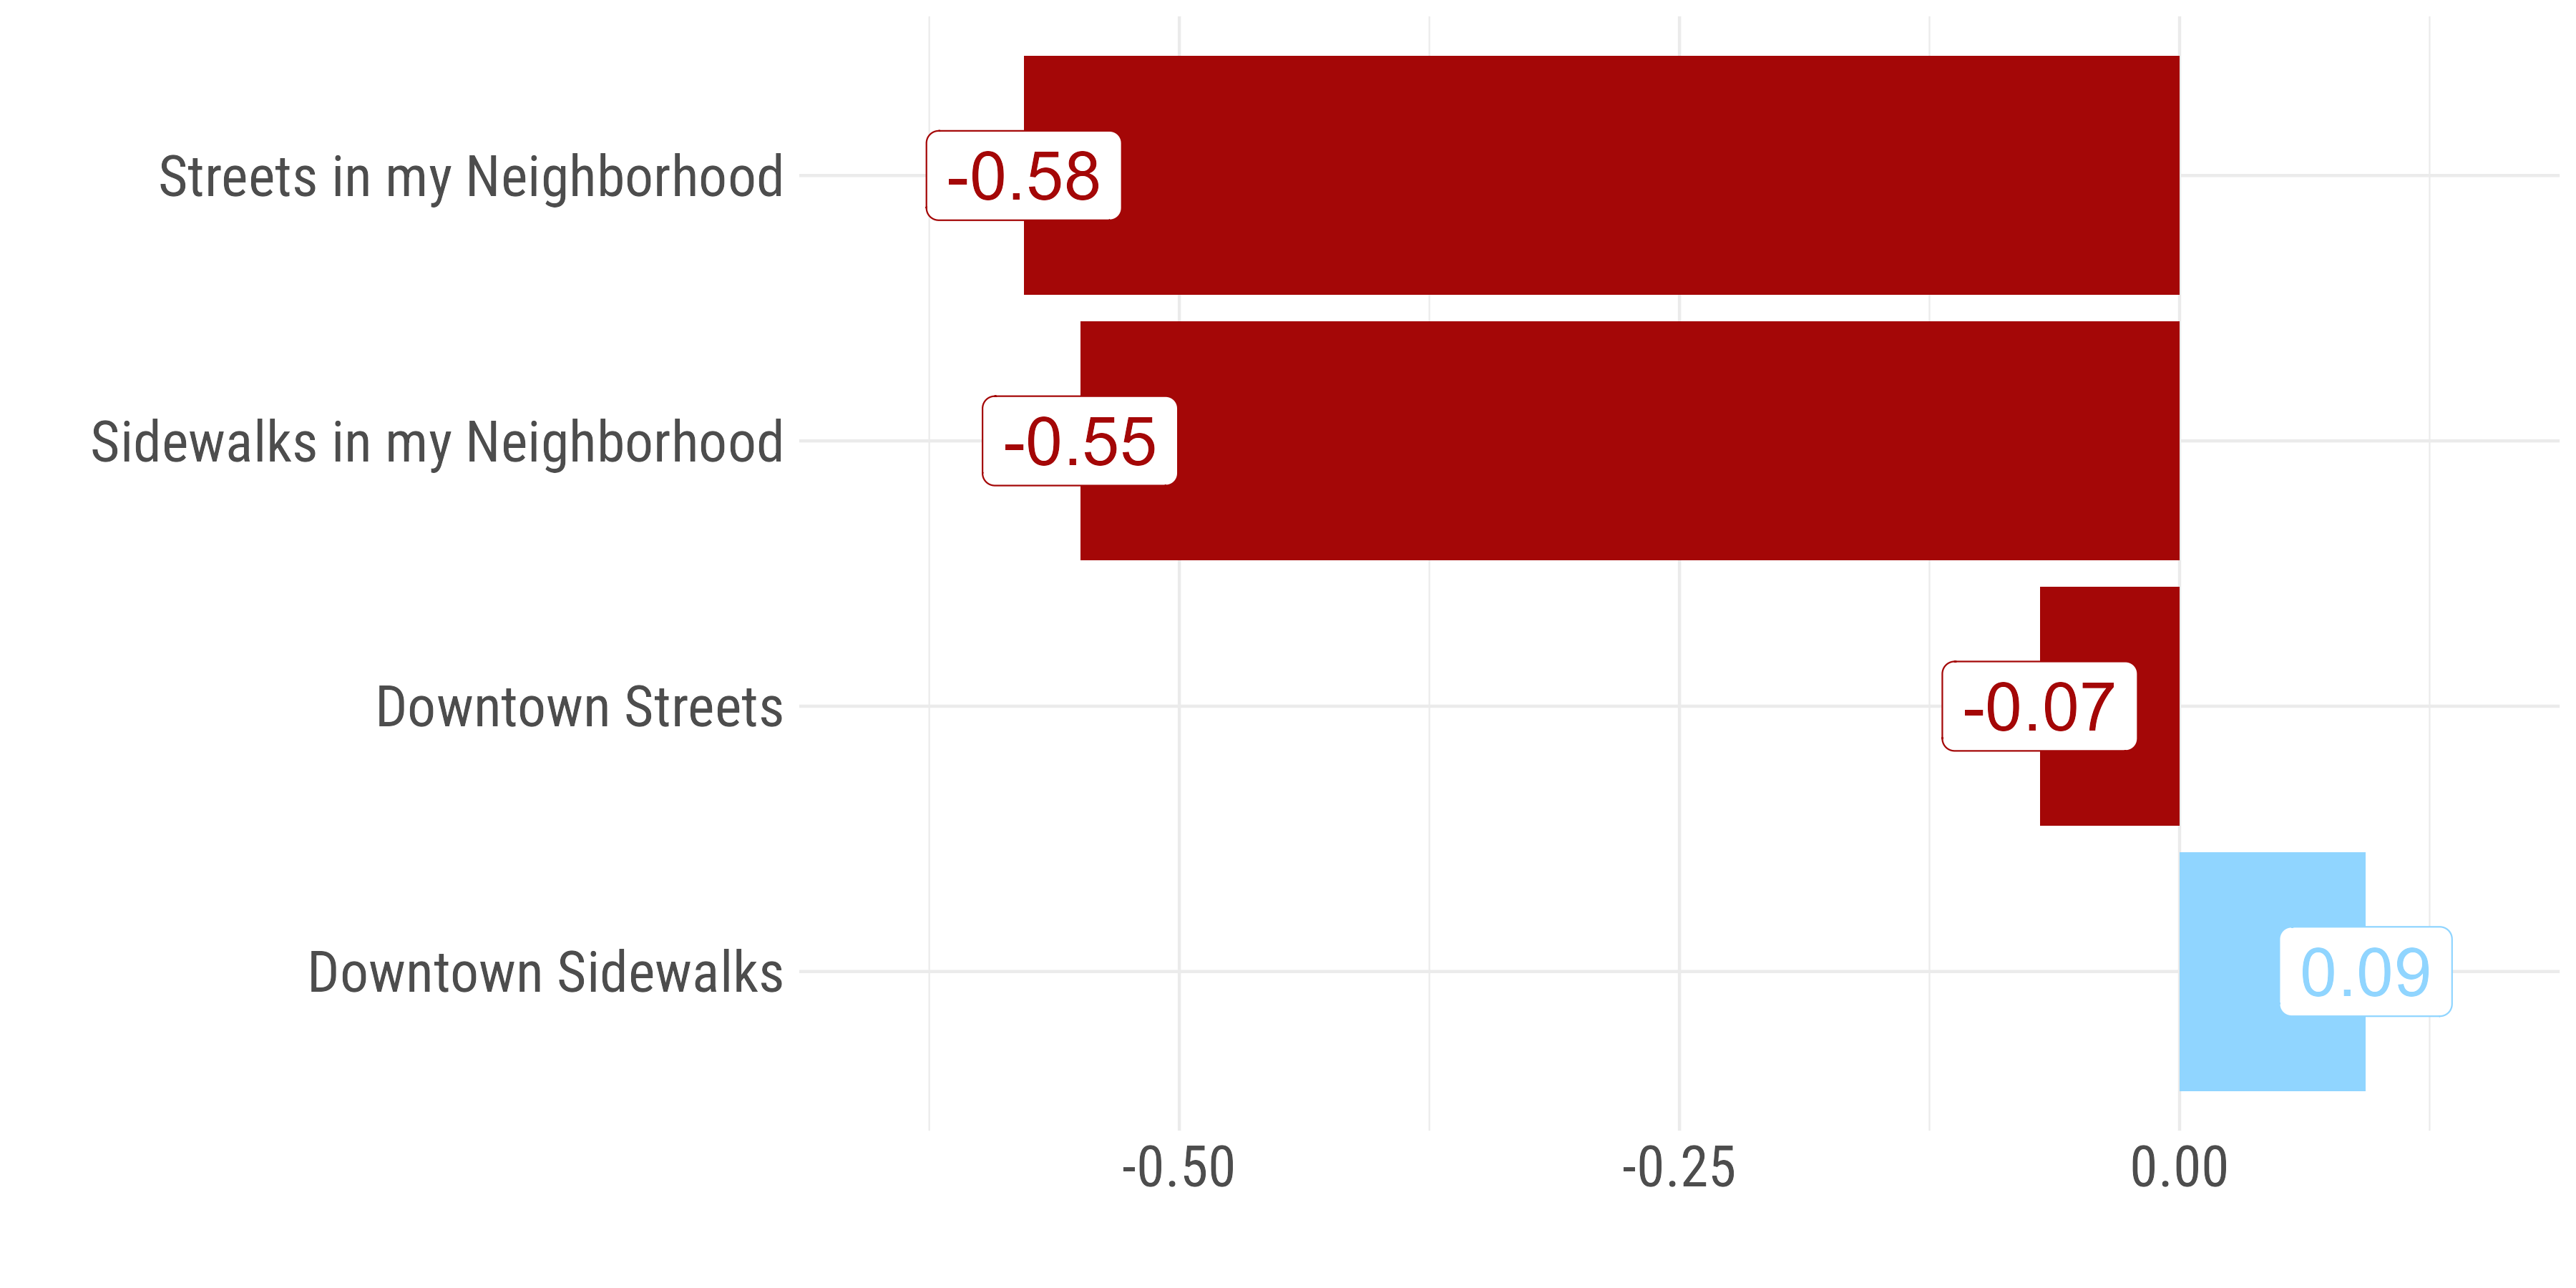
\includegraphics[width = \linewidth]{figures/score_streets_general.png}
\end{framed}
\end{figure}

\noindent Five Rule Rural Planning assessed street conditions in Bloomfield in \hl{[when??]}, creating a map of street conditions in Bloomfield. Our assessment of street conditions off Broadway Street and Highway 84 is similar: we assess that most of the streets in town are in need of some repair, although many of the roads in the southern half of town are in good condition.\\

\noindent In addition, we assessed sidewalk conditions in Bloomfield. Our assessment is similar to the residents'. Downtown sidewalks, near the intersection of Broadway Street and Highway 84, are mostly in good shape. However, Bloomfield residents gave a strong negative rating to sidewalks in their neighborhoods; our assessment is that this is because many neighborhoods do not have sidewalks at all, particularly in the southern half of Bloomfield.\\

\noindent We present our maps of Bloomfield's street and sidewalk conditions on the following pages.

\pagebreak
\thispagestyle{empty}
\begin{landscape}
    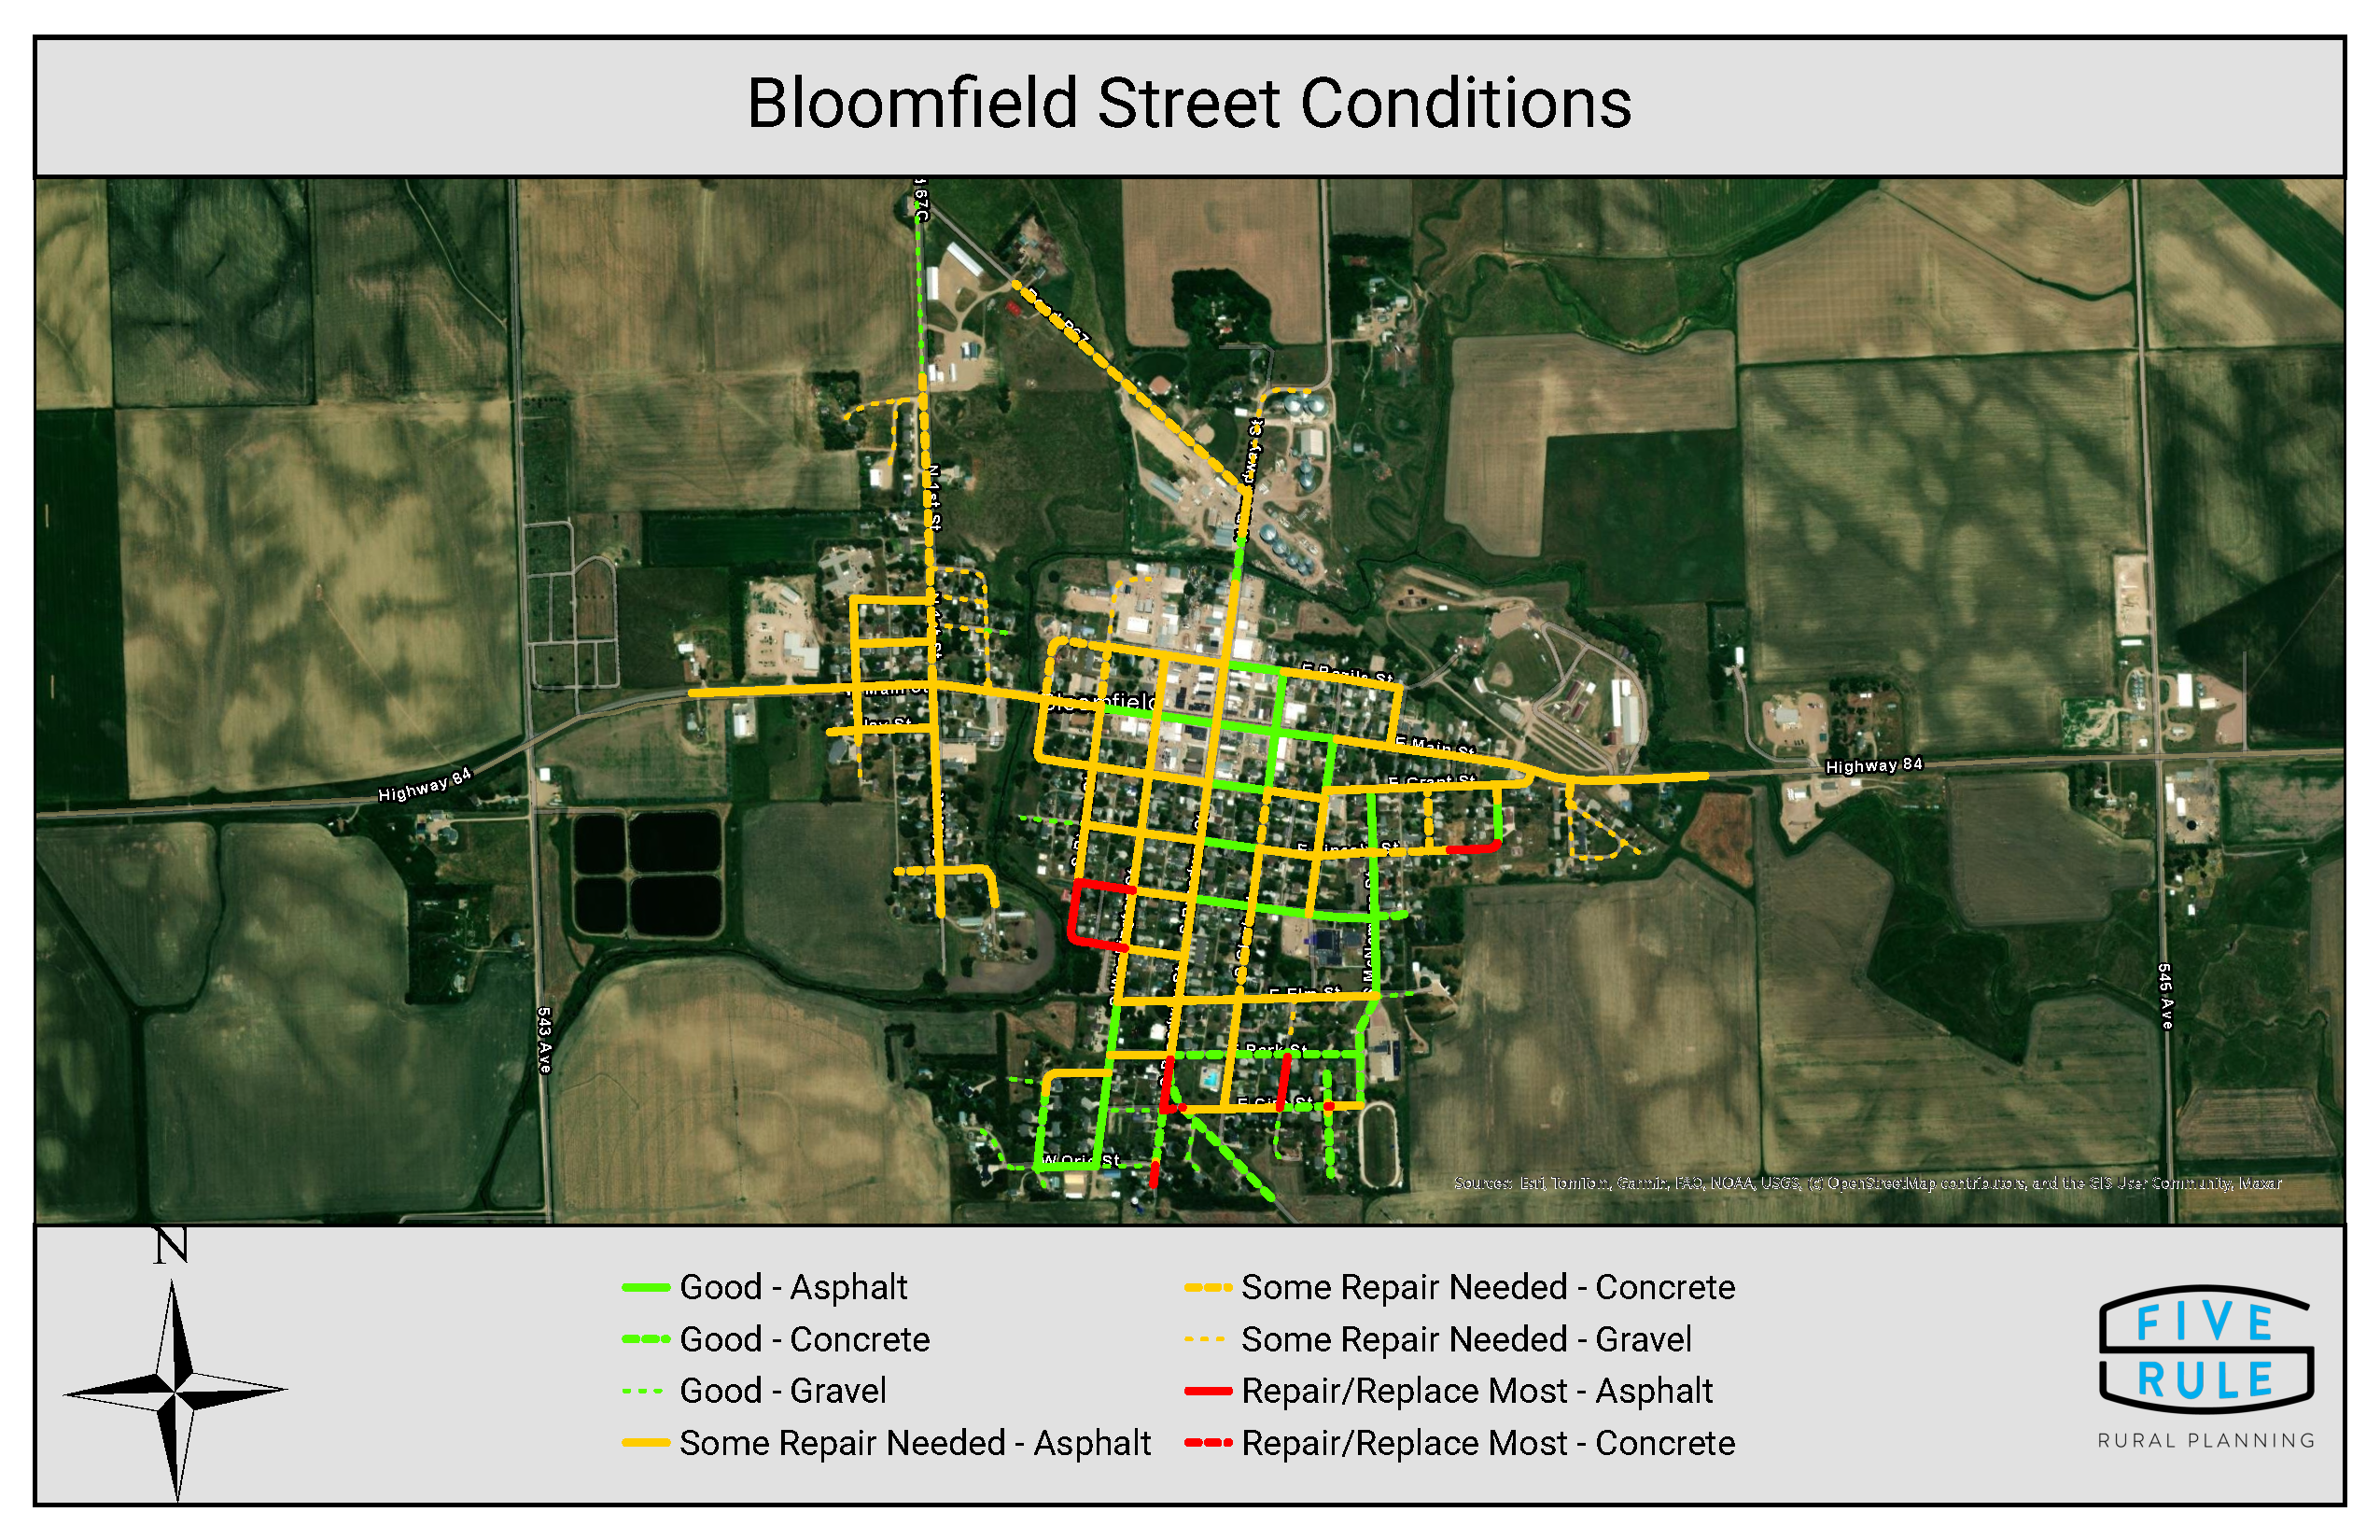
\includepdf[angle = 90]{maps/street_conditions.pdf}
\end{landscape}
\pagebreak

\pagebreak
\thispagestyle{empty}
\begin{landscape}
    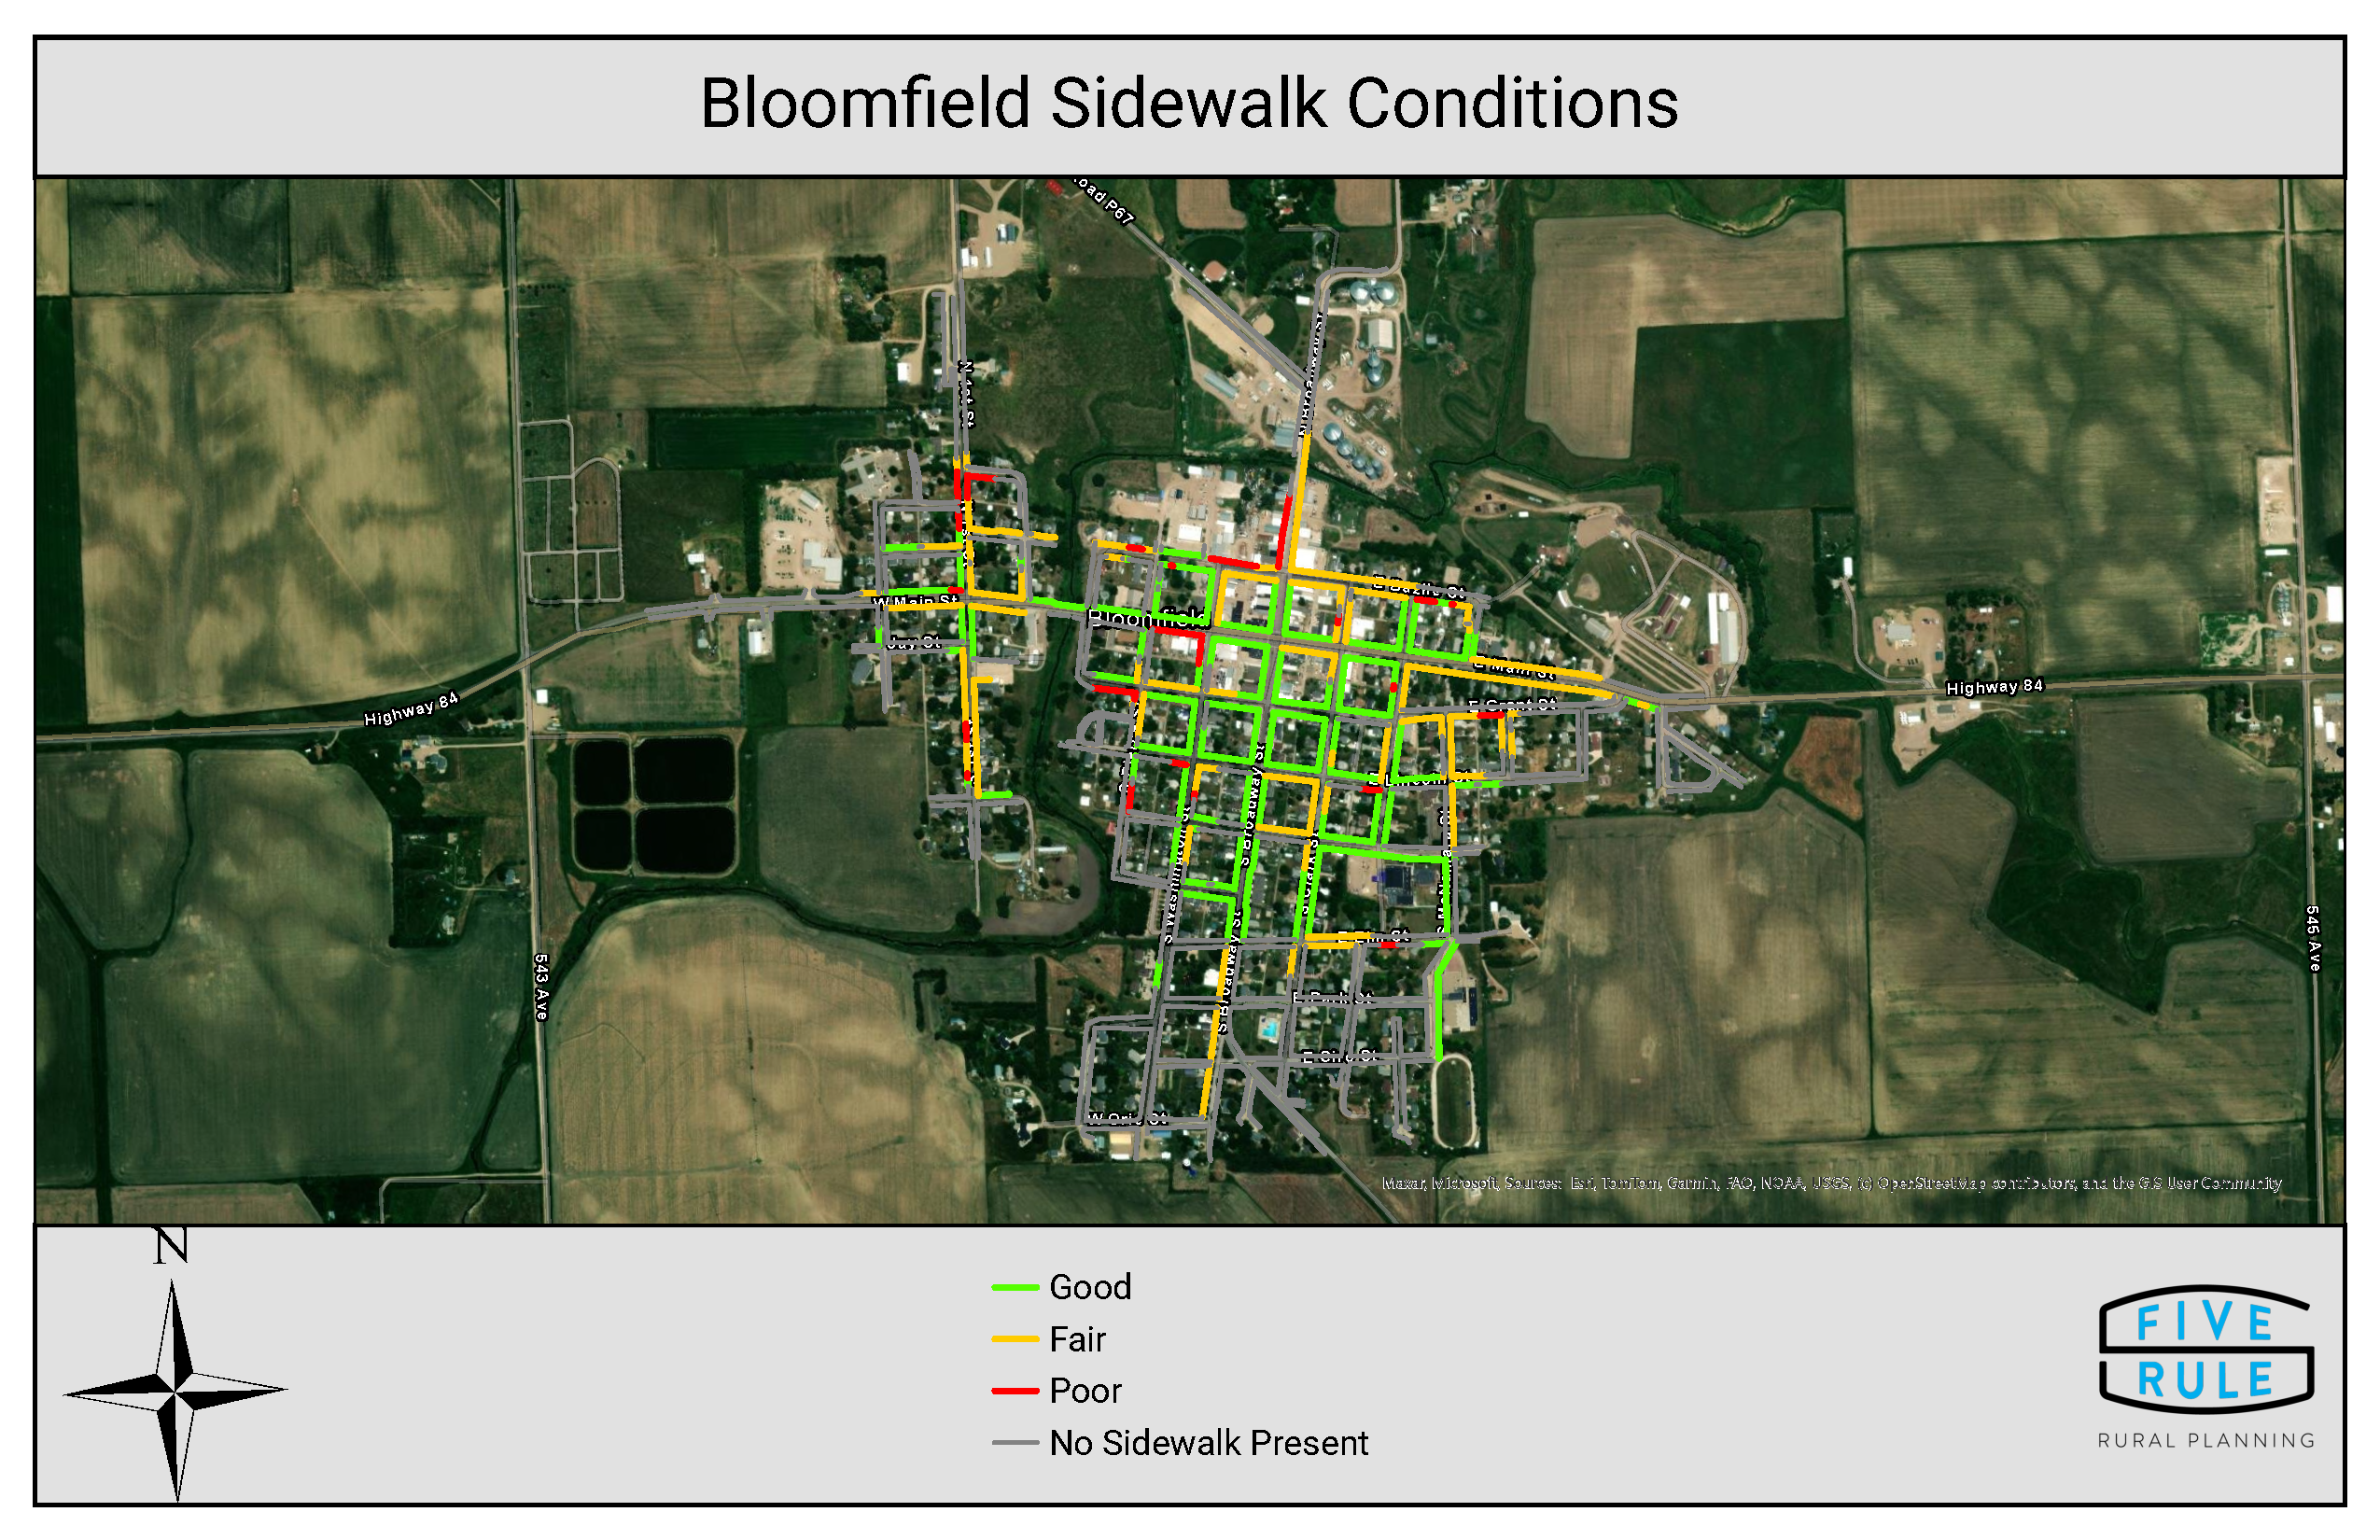
\includepdf[angle = 90]{maps/sidewalk_conditions.pdf}
\end{landscape}
\pagebreak

\subsection*{Key Takeaways}
\pagebreak
\section{City Utilities, Facilities, and Services}

\subsection{Water and Sanitation}

\noindent Second only to land availability, the provision of clean water and sanitary sewer services is the most important factor that impacts the city's ability to sustain itself and grow. Furthermore, utility services are important sources of city revenue. This is only possible if the customer base is growing and the rates charged to customers cover the cost of providing clean water and sanitation.\\

\noindent The \href{https://bloomfieldnebraska.com/government/}{City of Bloomfield Website} describes these utilities:

\subsubsection*{Water System}
\begin{quote}
    The city water system includes three supply wells with a total production capacity of approximately 1,000 gallons per minute. The average daily demand is 180,000 gallons with a maximum capacity of 1,440,000 per day. The static pressure is 93 pounds and the residual pressure is 86 pounds. The system also includes a single 250,000 elevated storage tank constructed in 1996. Extensive upgrades were undertaken in the water system between 1995 and 1997 resulting in an 8″ water line loop around the city. The quality of water in Bloomfield does not necessitate treatment.
\end{quote}

\subsubsection*{Sewer System}
\begin{quote}
    The wastewater system consists of approximately 6.9 miles of gravity collection mains, a satellite lift station in the east part of the city and a main lift station at the city park pumping all wastewater through a 3,200 foot 6″ force main to a four cell lagoon system. The collection system includes about 1,000 feet of 12″ main, 4,500 feet of 10″ main, 22,000 feet of 8″ main and 4,200 feet of 4″ main. The four cell lagoon is operated as a controlled discharge system and was upgraded within the last 10 years. It meets the state NPDES limits on effluent. Renovations of the main lift station and collection system are being done in 2000, including a new lift station on the west side of the city.
\end{quote}

\pagebreak
\noindent On the whole, Bloomfield residents are more satisfied than dissatisfied with the provision of water and sewer utilities. \textbf{Figure~\ref{fig:scoreWaterSewer}} shows that Bloomfield residents were 18 percent more likely to rate the city water service as "good" or better, and 14 percent more likely to rate the city sewer service as "good" or better.

\begin{figure}[H]
\centering
\begin{framed}
    \caption{Assessment of Water and Sewer Utilities}
    \label{fig:scoreWaterSewer}
    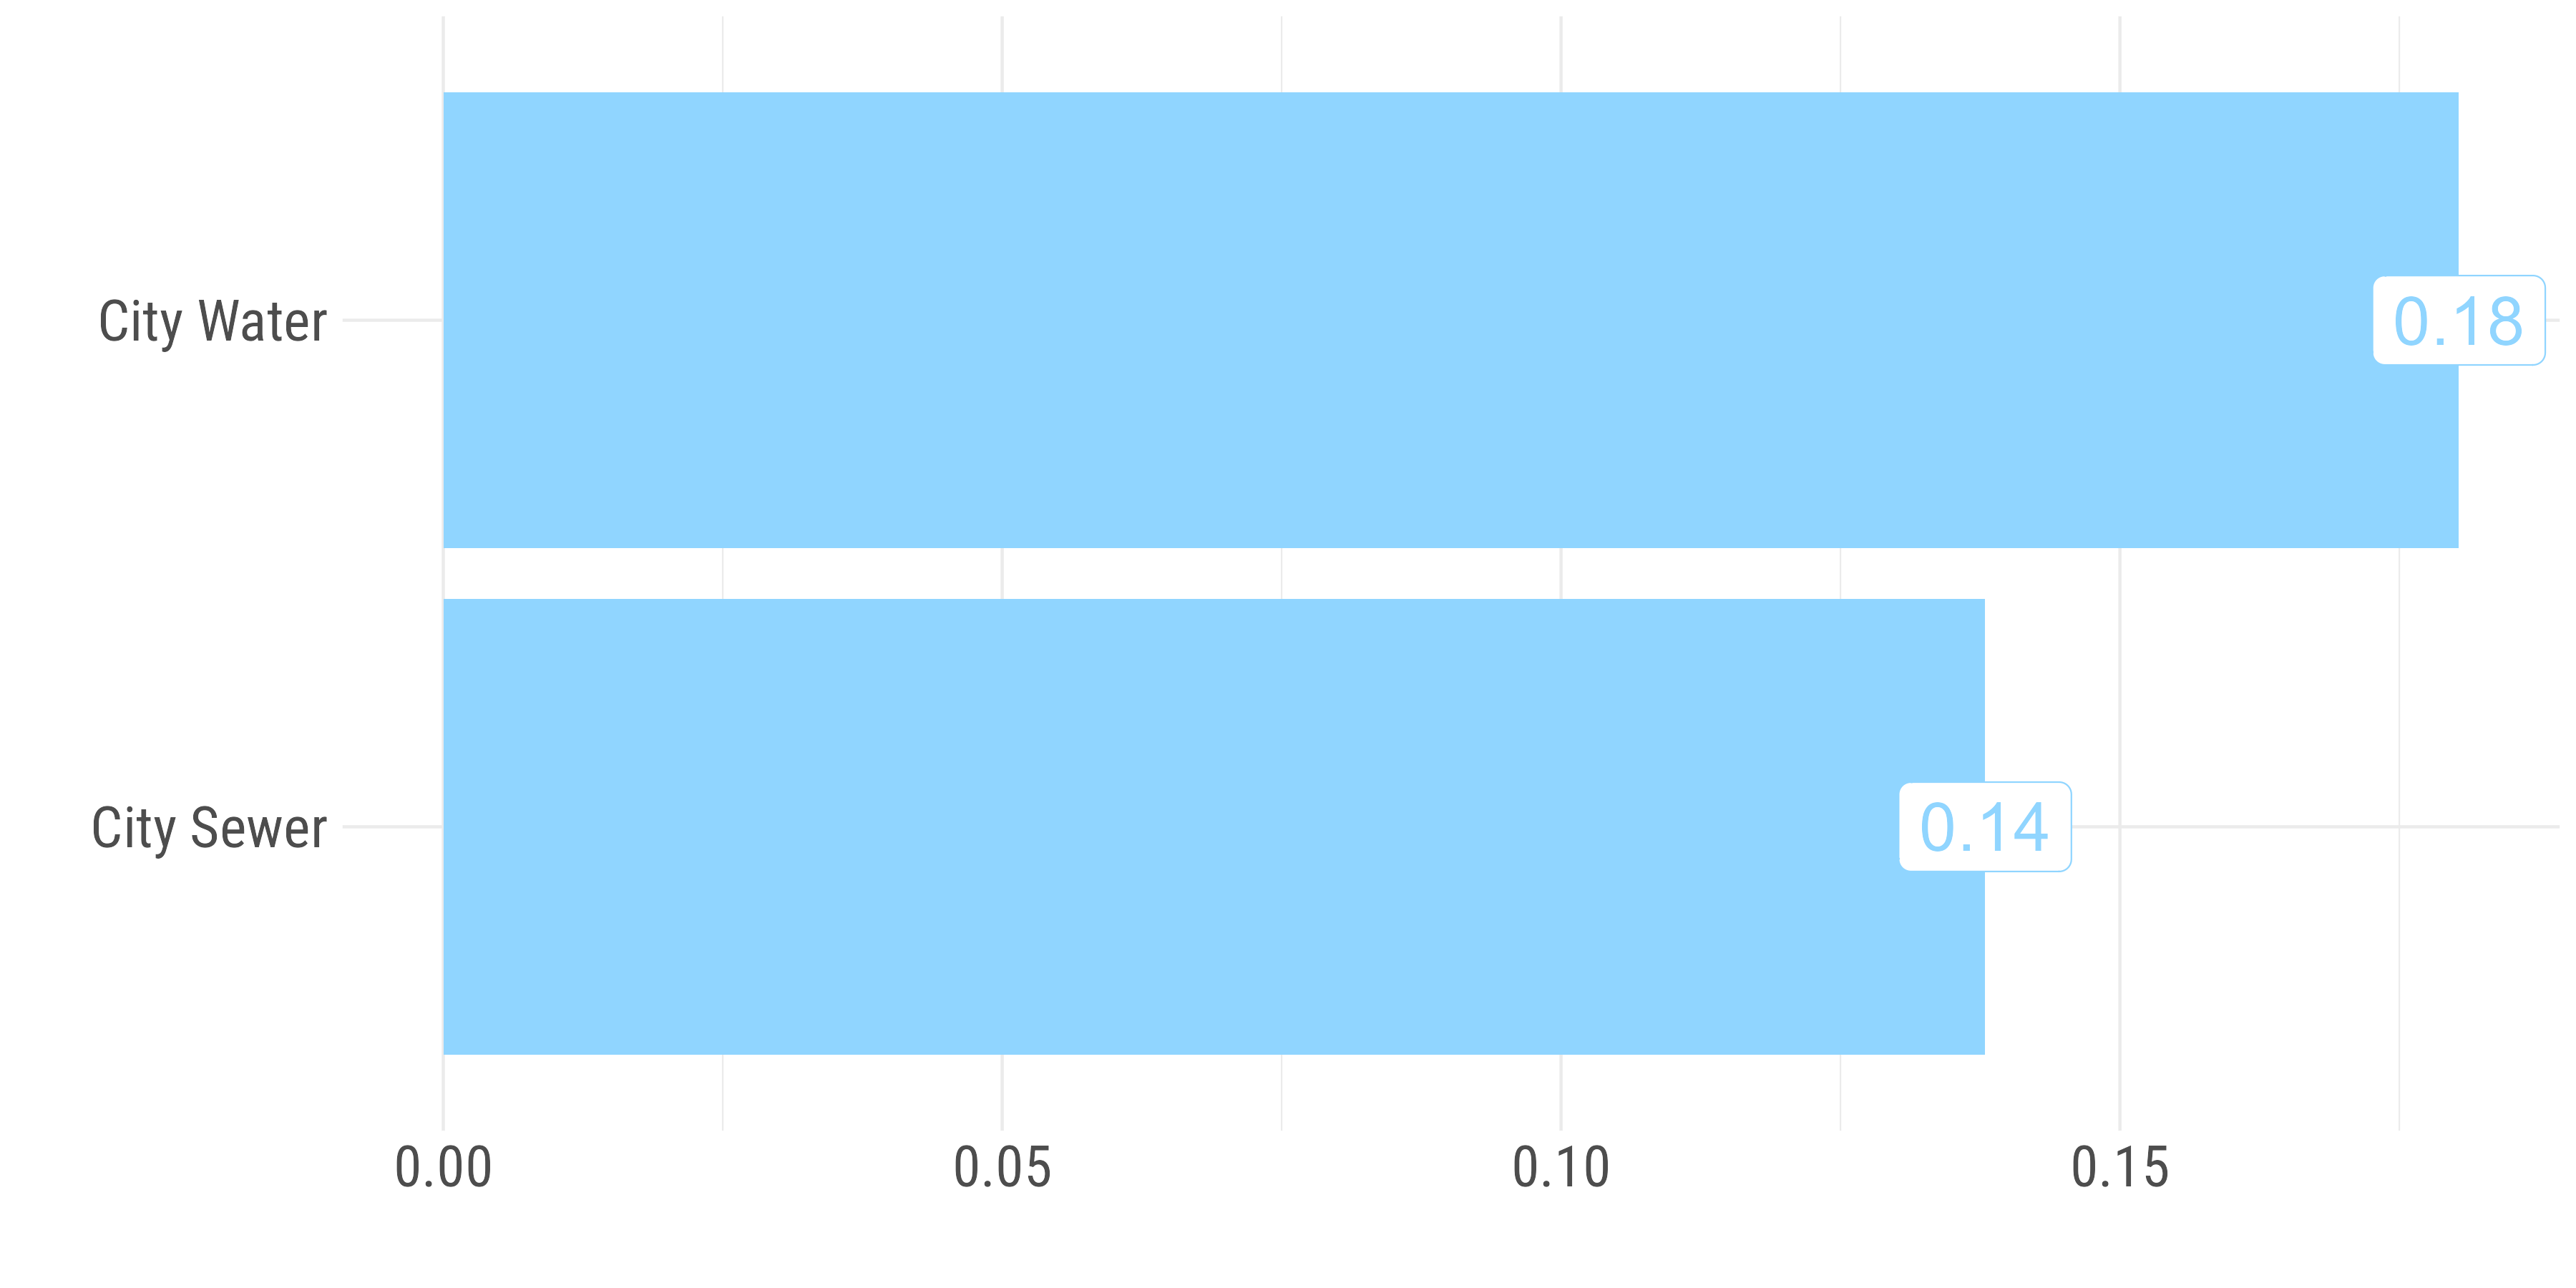
\includegraphics[width = \linewidth]{figures/score_water_sewer.png}
\end{framed}
\end{figure}

\noindent The maps on the following pages detail the location of Bloomfield's water and sewer infrastructure.

\pagebreak
\thispagestyle{empty}
\begin{landscape}
    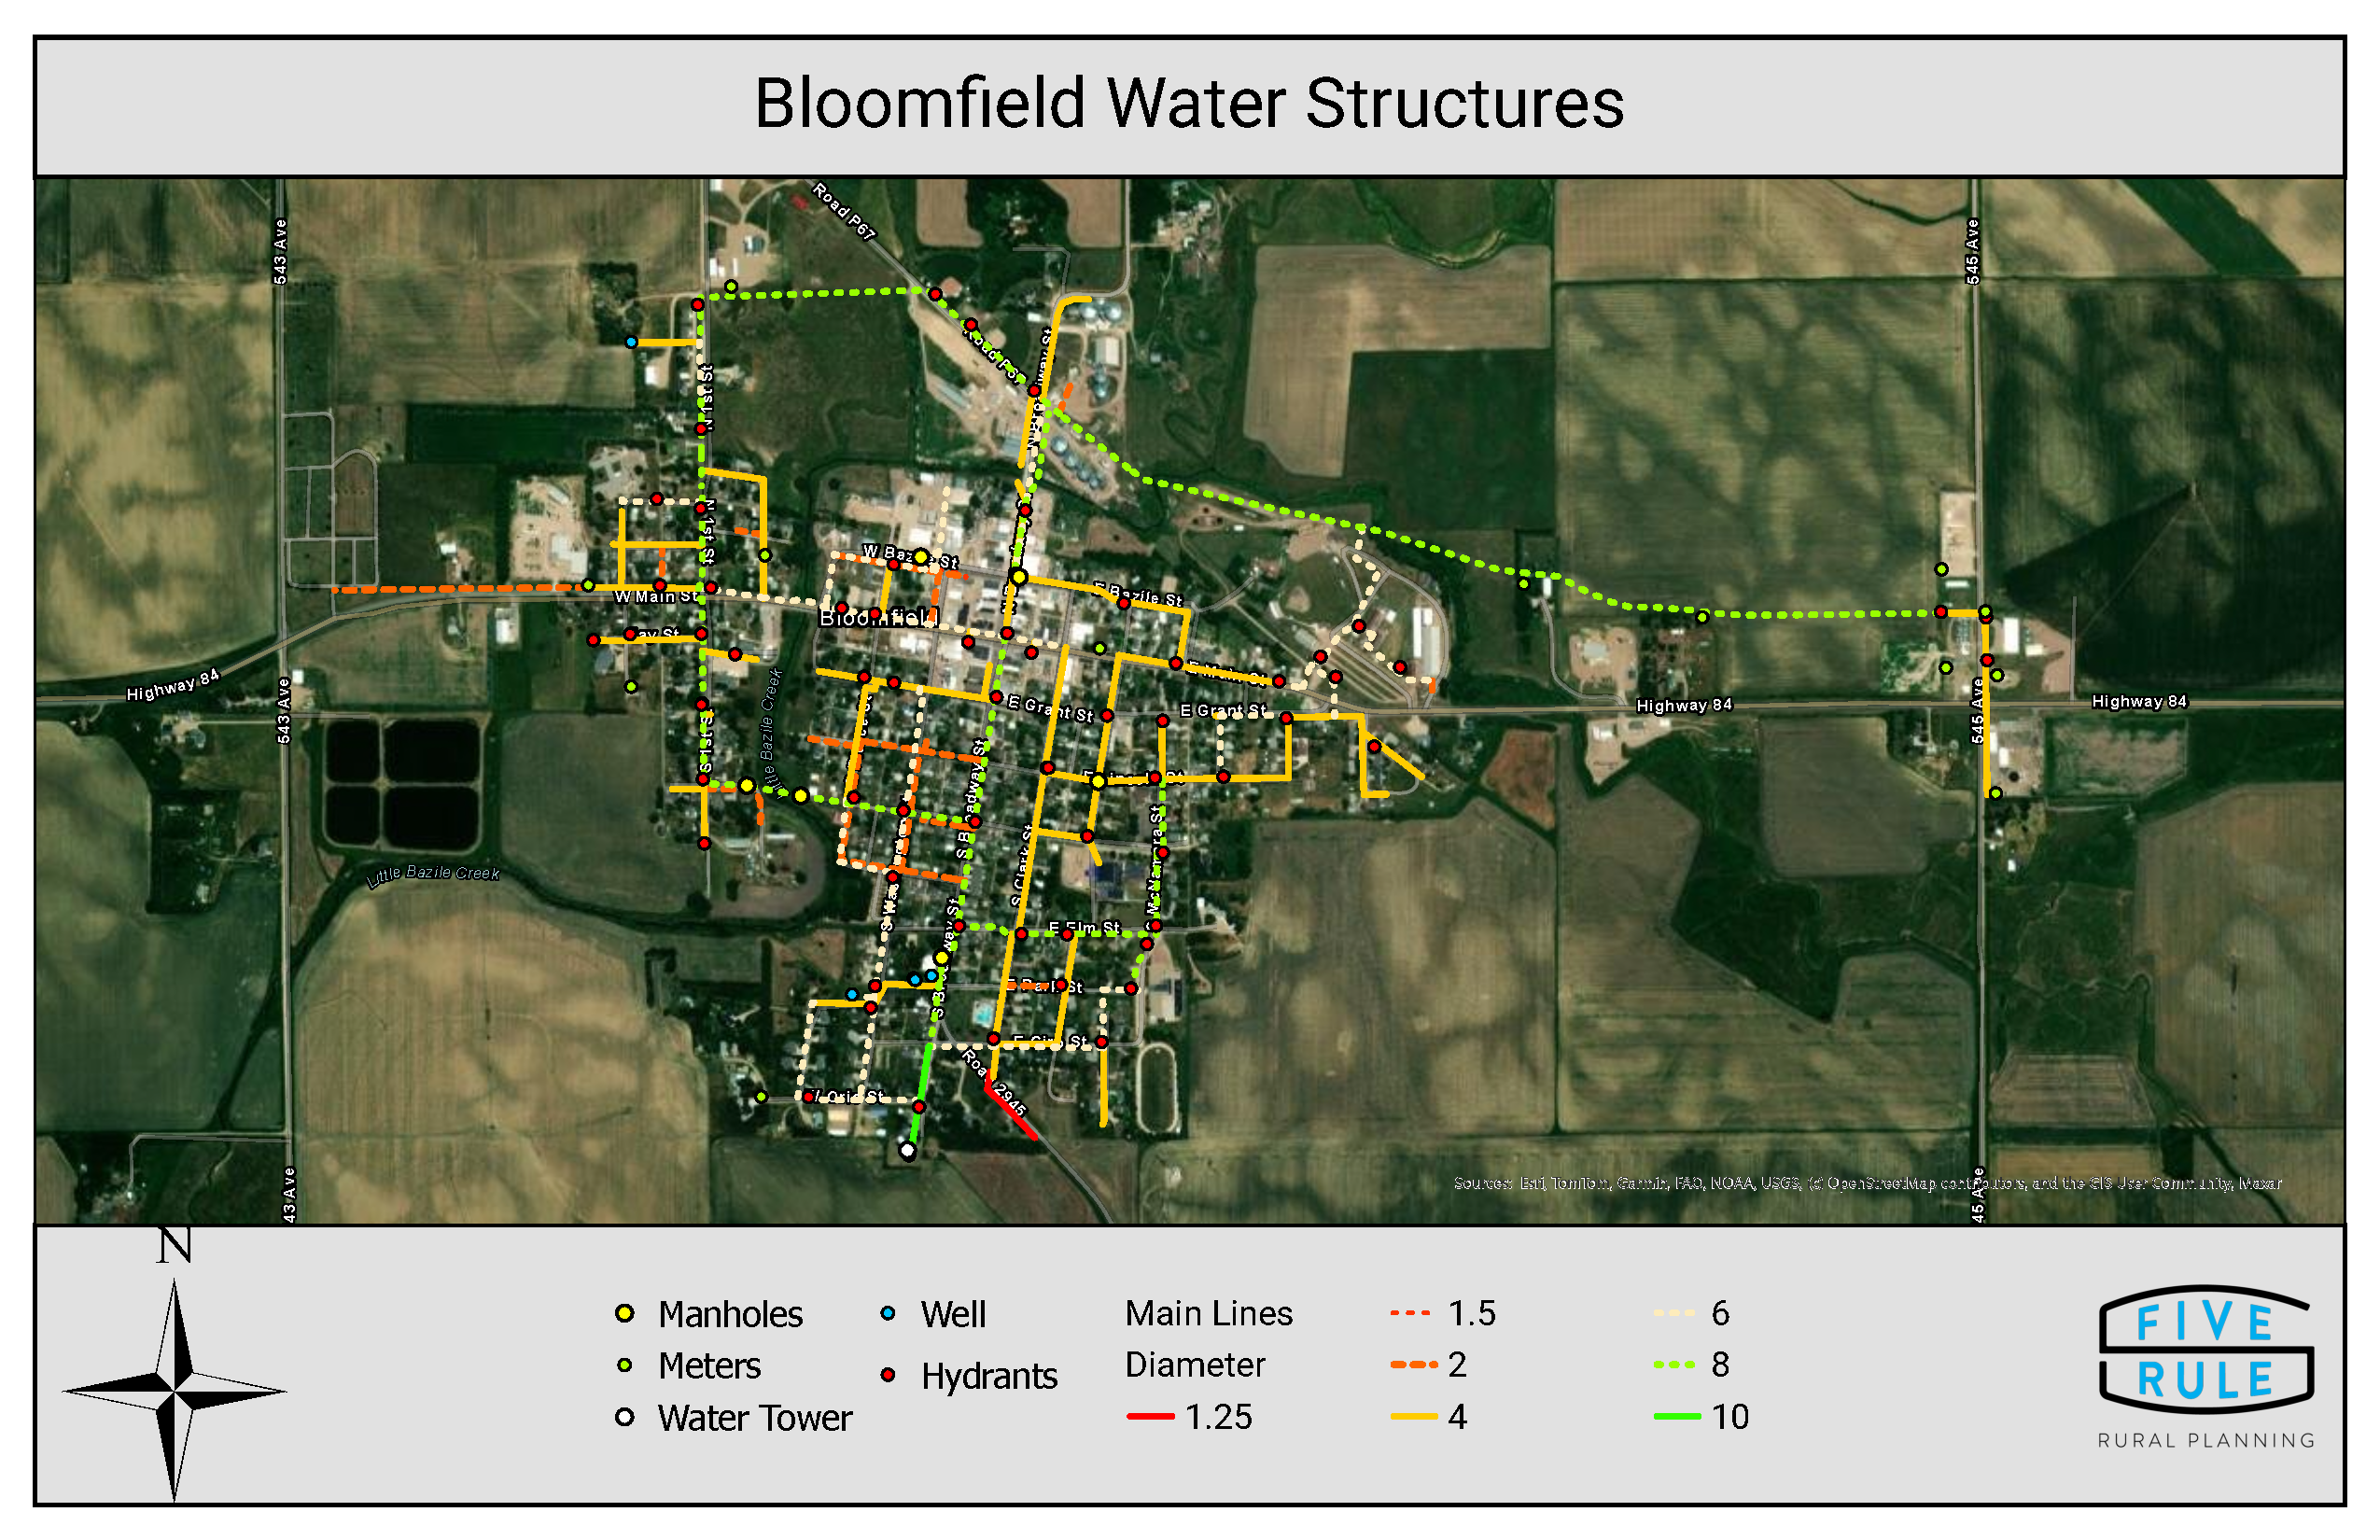
\includepdf[angle = 90]{maps/water_structures.pdf}
\end{landscape}

\pagebreak
\thispagestyle{empty}
\begin{landscape}
    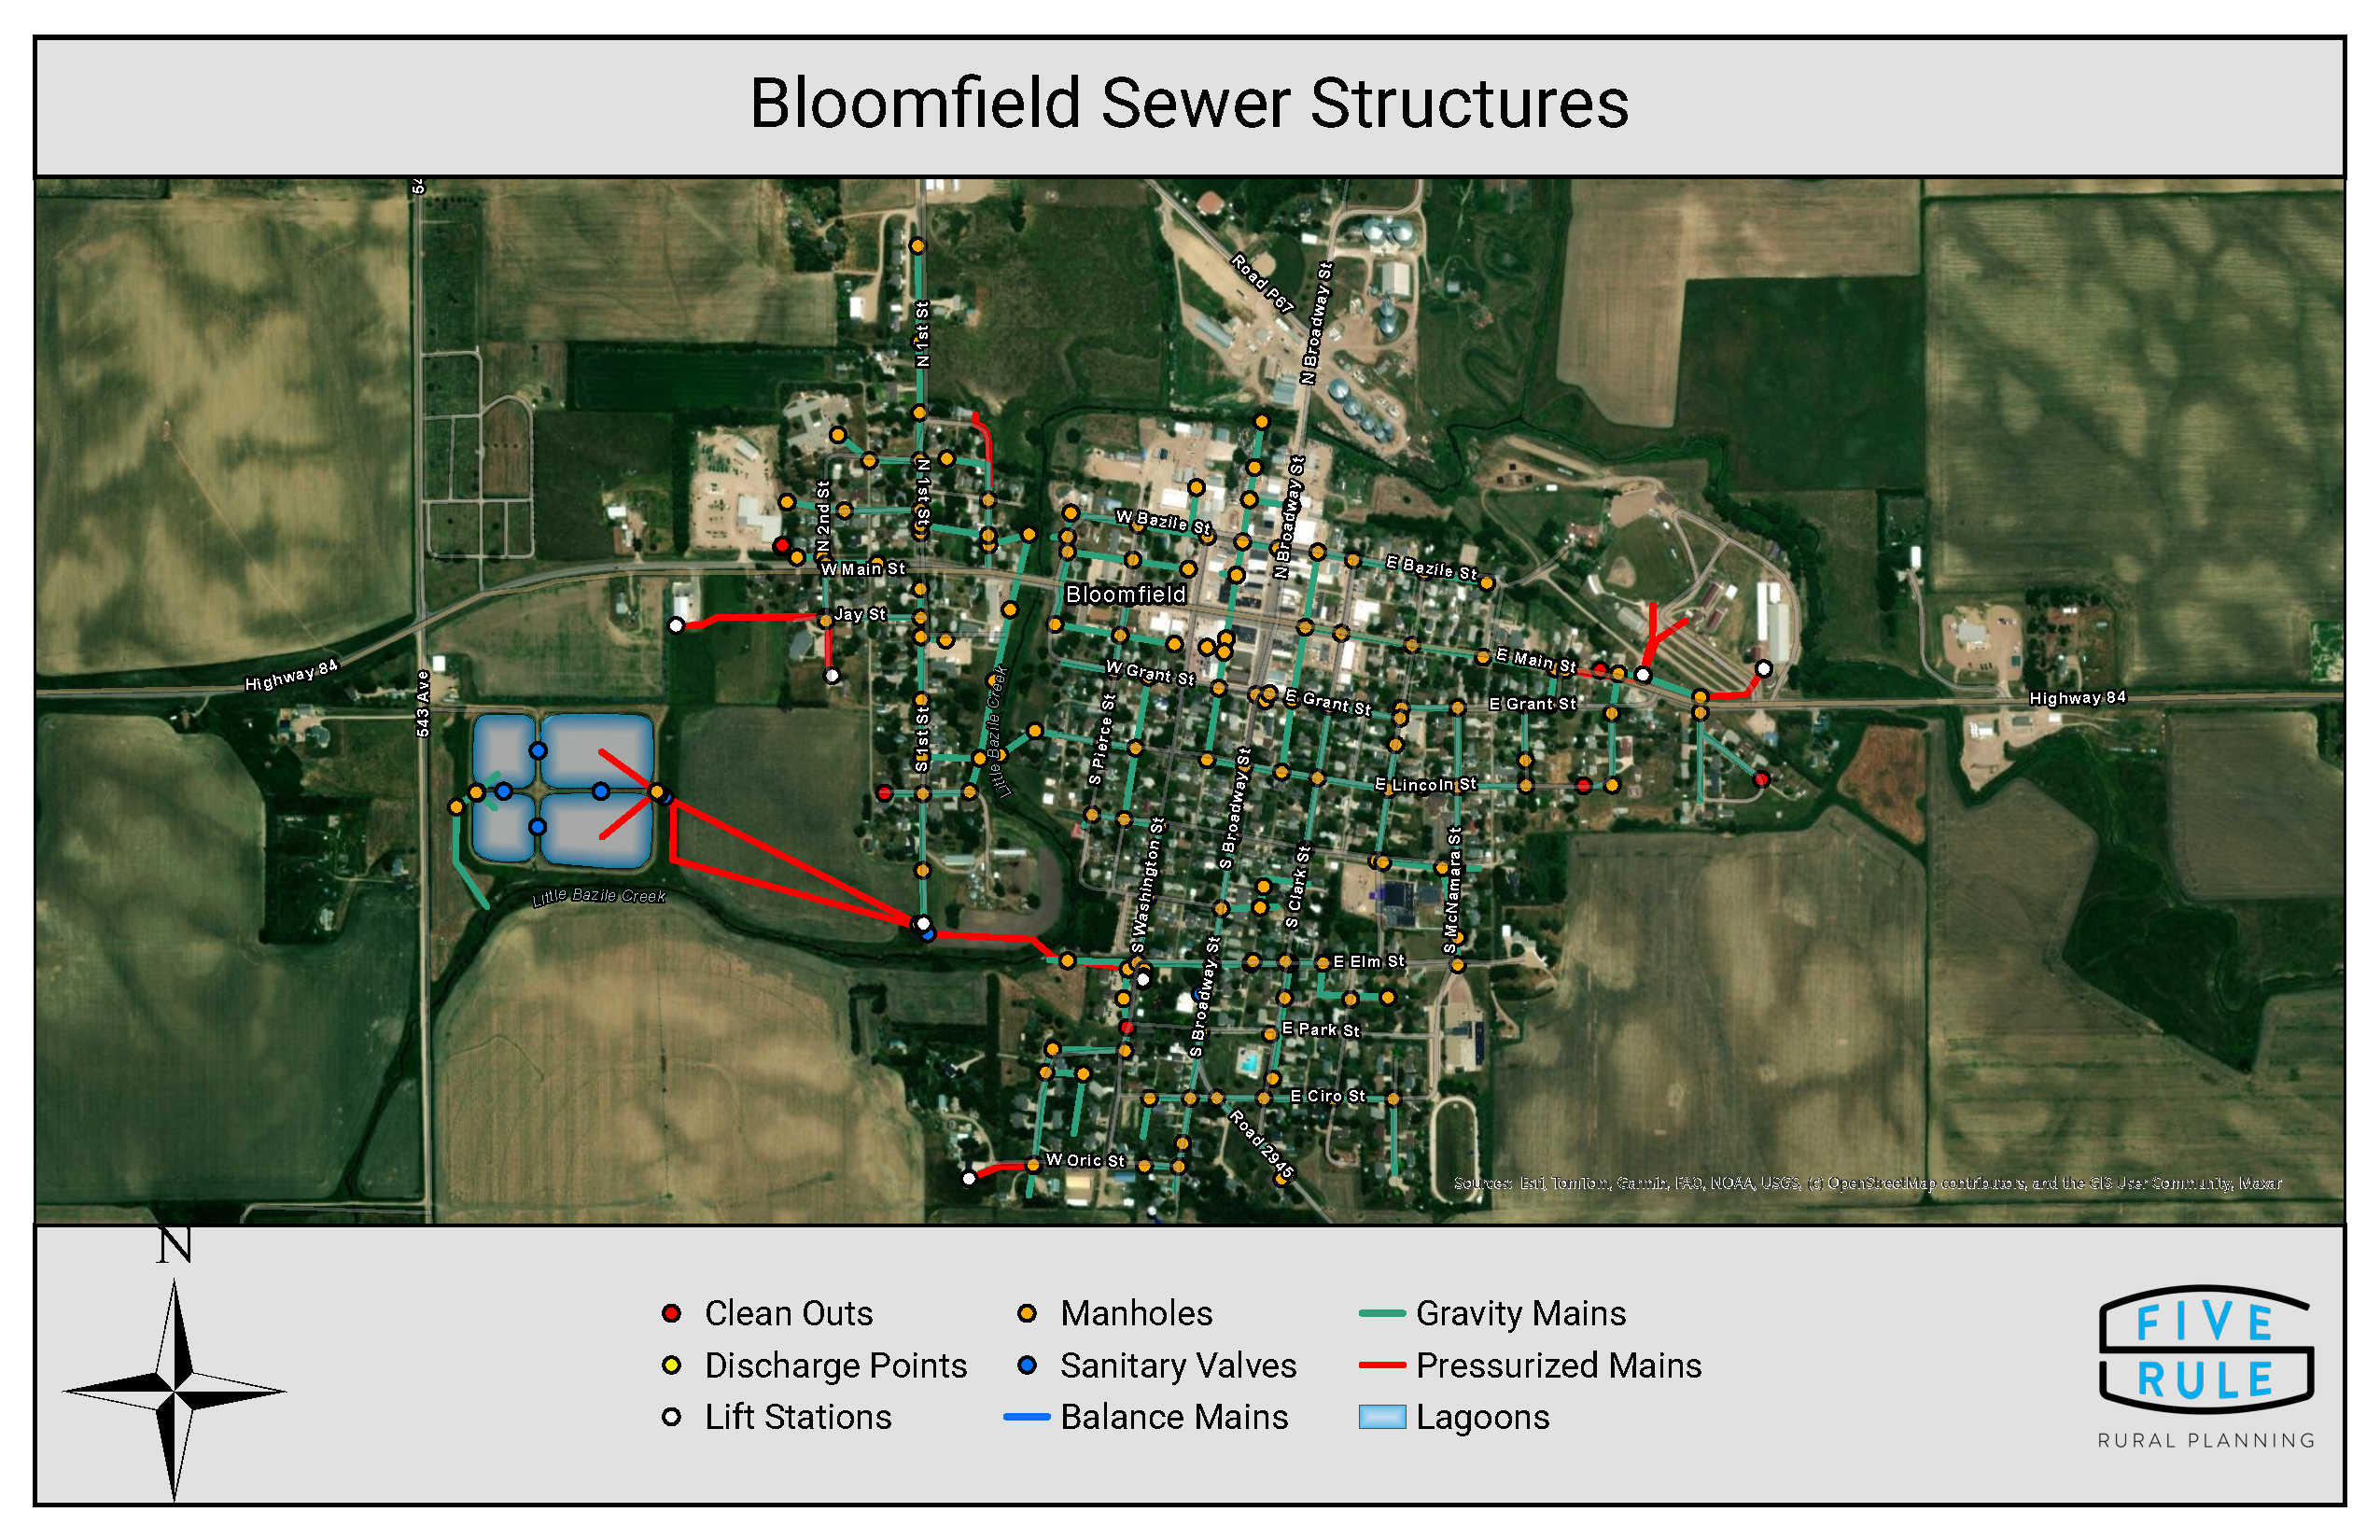
\includepdf[angle = 90]{maps/sewer_structures.pdf}
\end{landscape}

\pagebreak
\subsection{Energy Element}

\noindent As a reminder, \href{https://nebraskalegislature.gov/laws/statutes.php?statute=19-903}{NRS \S 19-903(4)} stipulates:

\begin{quote}
    (4) When a new comprehensive plan or a full update to an existing comprehensive plan is developed, an energy element which: Assesses energy infrastructure and energy use by sector, including residential, commercial, and industrial sectors; evaluates utilization of renewable energy sources; and promotes energy conservation measures that benefit the community.
\end{quote}

\noindent According to the \href{https://bloomfieldnebraska.com/government/}{Bloomfield City Government}, city residents have access to two sources of energy: electricity and natural gas. From the website:
\begin{quote}
"Electric service is supplied and distributed by the Nebraska Public Power District (NPPD). The nearest substation is located on the east edge of the community. The Bloomfield area is serviced by two different 69 KV lines. The transmission size to the substation is 69 KV and the substation capacity is 4160 KV with the distribution transformer approximately 60 percent loaded at the present. Two additional substations are located within five miles of Bloomfield. Service and maintenance is provided from the NPPD office in Norfolk."

Natural gas service is distributed and supplied to the community by SourceGas, through a three-inch transmission pipeline with an operating pressure of approximately 800-900 pounds per square inch. Choice Gas is available in Bloomfield and the election period for this program is prior to May 1st of each year.
\end{quote}

\noindent Most of Knox County's energy demand will be satisfied primarily by electricity and natural gas. Electricity consumption currently accounts for about two-thirds (68\%) of county consumption. By 2050, it is projected that share will increase to about three quarters (76\%). Furthermore, total costs are likely to increase for electricity but decrease or remain about the same for natural gas. As technology improves, electricity efficiency is likely to improve, driving per-unit costs down. On the other hand, natural gas efficiency is likely to get worse, driving per-unit costs up.

\begin{table}[H] 
\begin{framed}
\centering \doublespacing
  \caption{Knox County Energy Estimates}
  \label{table:energy}
 \scalebox{1.00}{
\begin{tabular}{l D{.}{.}{8.5} D{.}{.}{8.5} D{.}{.}{8.5}} \hline
\multicolumn{1}{c}{Year}& \multicolumn{1}{c}{Source} & \multicolumn{1}{c}{Consumption}  & \multicolumn{1}{c}{Cost}  \\ \hline
2020    & \multicolumn{1}{c}{Electricity}   & \multicolumn{1}{c}{197,390}   & \multicolumn{1}{c}{\$4,922,145}   \\
2020    & \multicolumn{1}{c}{Natural Gas}   & \multicolumn{1}{c}{93,489}    & \multicolumn{1}{c}{\$616,114}     \\
2030    & \multicolumn{1}{c}{Electricity}   & \multicolumn{1}{c}{208,019}   & \multicolumn{1}{c}{\$4,785,416}   \\
2030    & \multicolumn{1}{c}{Natural Gas}   & \multicolumn{1}{c}{85,745}    & \multicolumn{1}{c}{\$623,816}     \\
2040    & \multicolumn{1}{c}{Electricity}   & \multicolumn{1}{c}{227,321}   & \multicolumn{1}{c}{\$5,097,271}   \\
2040    & \multicolumn{1}{c}{Natural Gas}   & \multicolumn{1}{c}{80,929}    & \multicolumn{1}{c}{\$618,994}     \\
2050    & \multicolumn{1}{c}{Electricity}   & \multicolumn{1}{c}{252,633}   & \multicolumn{1}{c}{\$5,426,186}   \\
2050    & \multicolumn{1}{c}{Natural Gas}   & \multicolumn{1}{c}{78,031}    & \multicolumn{1}{c}{\$641,611}     \\
\hline
\end{tabular}
}
\floatnote{Data come from the \href{https://maps.nrel.gov/slope/data-viewer?filters=\%5B\%5D&layer=energy-consumption.net-electricity-and-natural-gas-consumption&year=2020\&res=county}{United States Department of Energy State and Local Planning for Energy database}. Consumption estimates are in Millions of British Thermal Units (MMBtu), while cost estimates are in nominal United States dollars.}
\end{framed}
\end{table}

\noindent In Nebraska, energy use is categorized according to land use. \textbf{Commercial energy} is used by non-manufacturing business establishments. This includes restauants, wholesale businesses, retail stores, and other service enterprises. Institutional and government offices and facilities are also included in the commercial sector, as well as streetlights, pumps, bridges, and other public services. \textbf{Residential energy} refers to energy used for private household functions, such as heating spaces, heating water, air conditioning, refrigeration, cooking, laundry, and lighting. \textbf{Figure~\ref{fig:energyElement}} displays projected energy consumptions and costs in Knox County between 2017 and 2050 across different land use categories.

\begin{figure}[H]
\centering
\begin{framed}
    \caption{Knox County Projected Energy Uses}
    \label{fig:energyElement}
     \begin{subfigure}{0.49\textwidth}
        \centering
        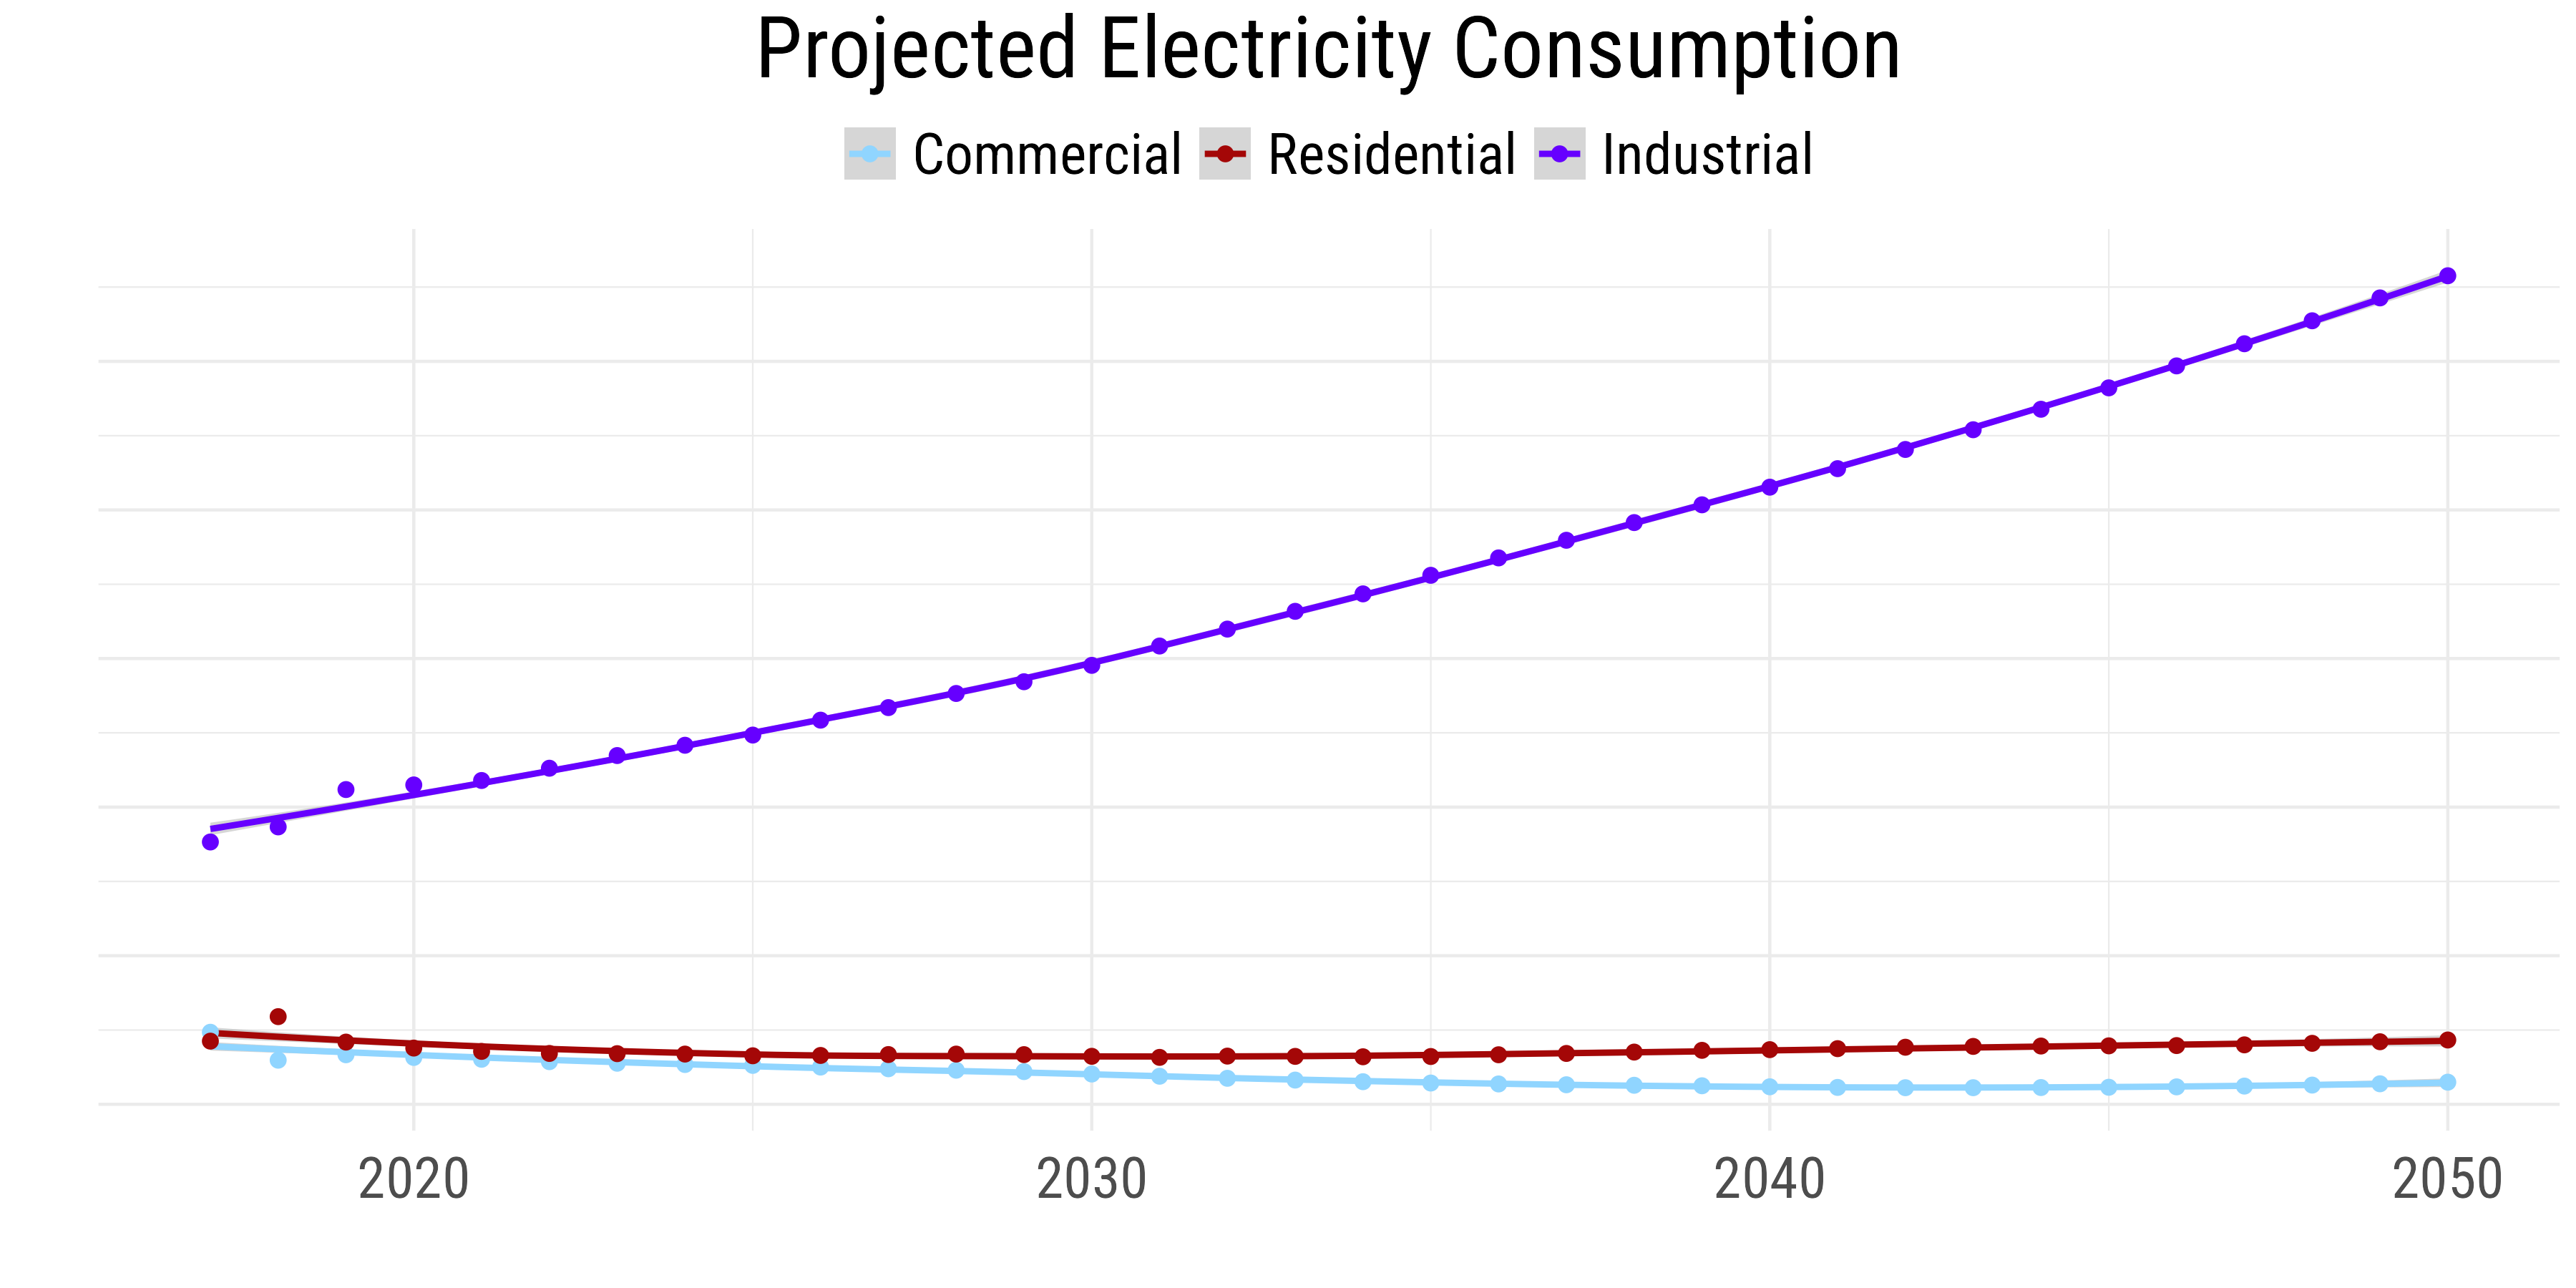
\includegraphics[width=\linewidth]{figures/energy_consumption_elec.png}
     \end{subfigure}
     \begin{subfigure}{0.49\textwidth}
        \centering
        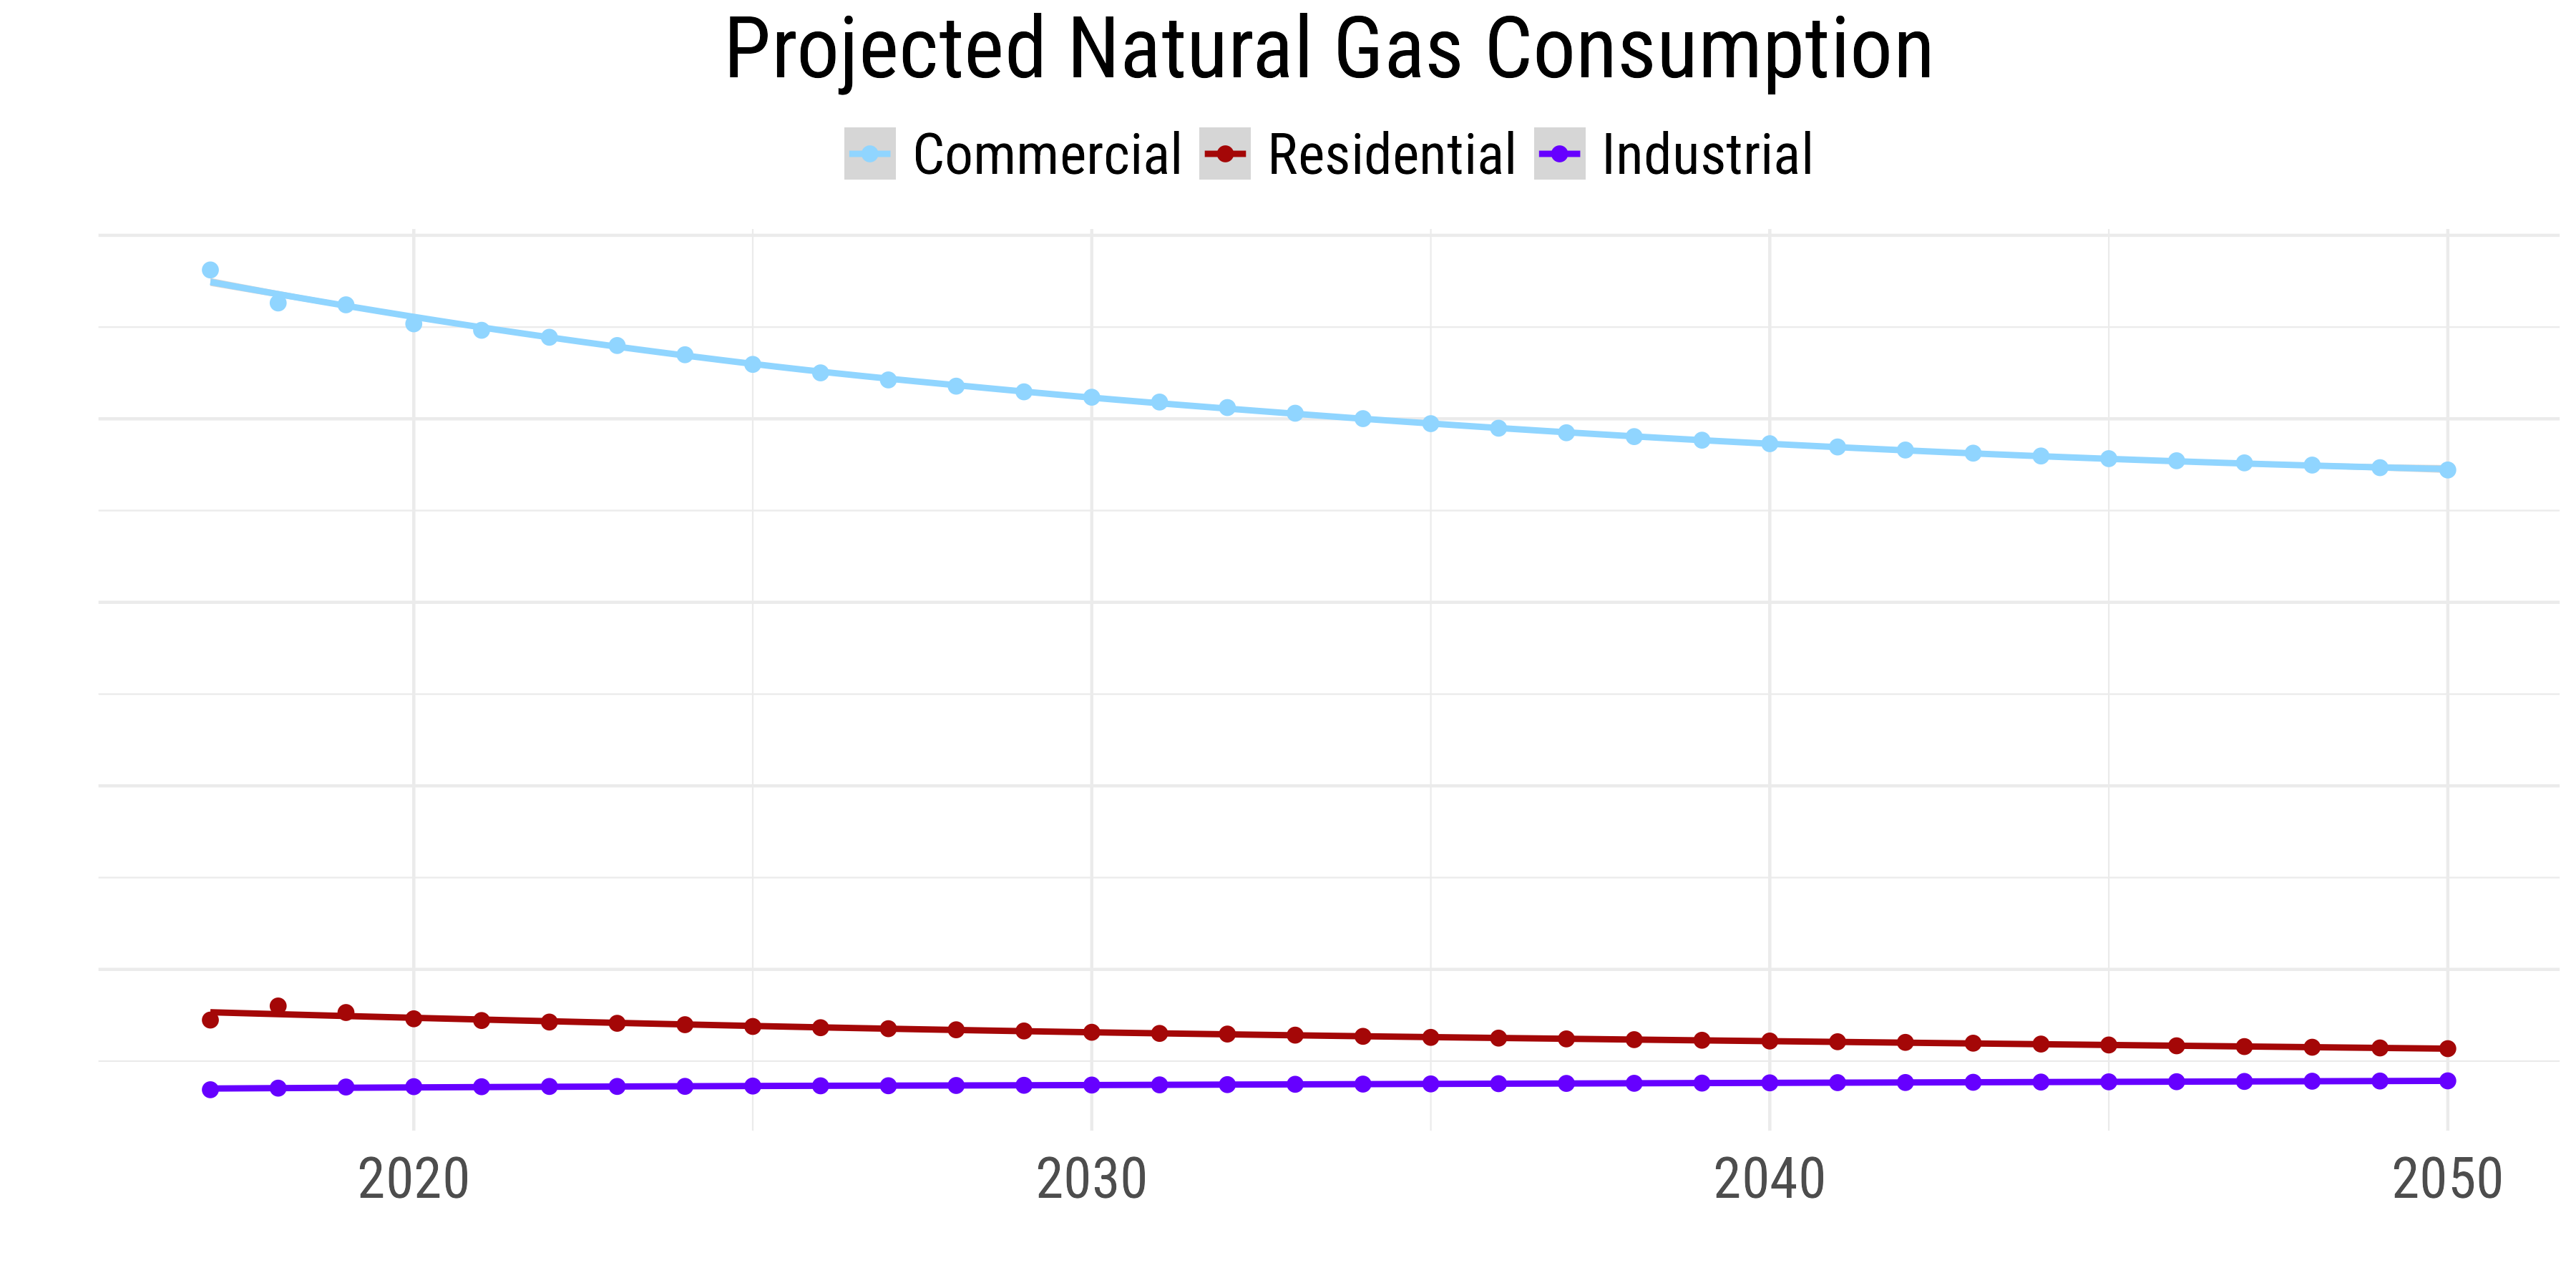
\includegraphics[width=\linewidth]{figures/energy_consumption_ng.png}
     \end{subfigure}
     \begin{subfigure}{0.49\textwidth}
        \centering
        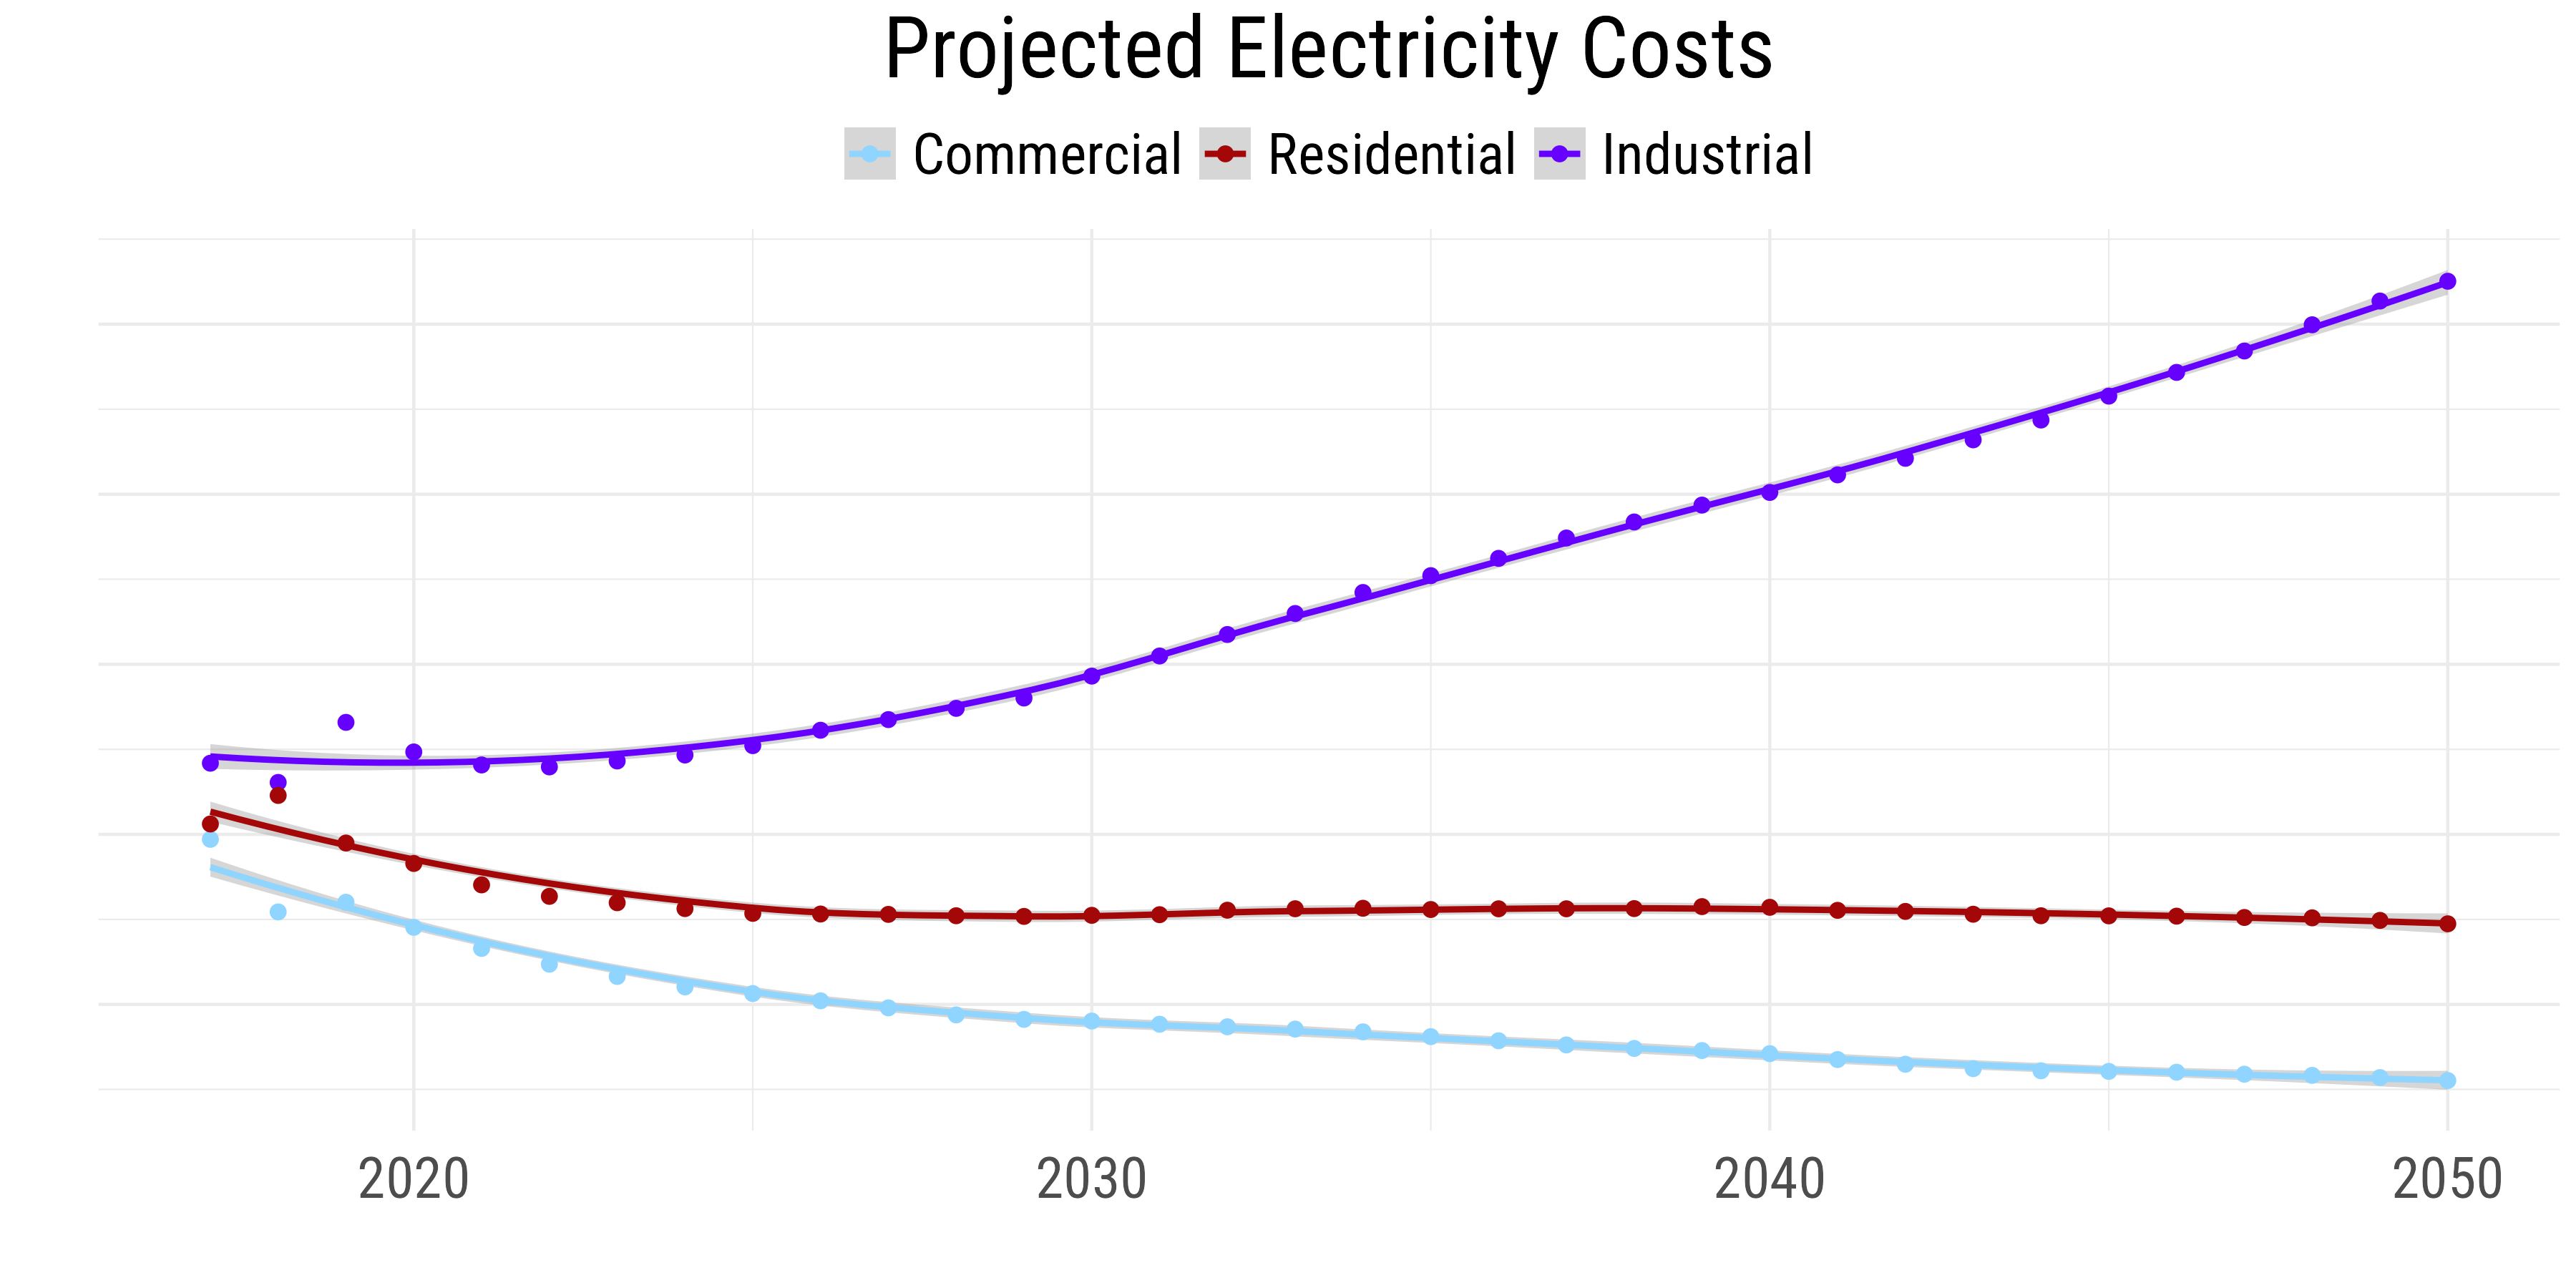
\includegraphics[width=\linewidth]{figures/energy_cost_elec.png}
     \end{subfigure}
     \begin{subfigure}{0.49\textwidth}
        \centering
        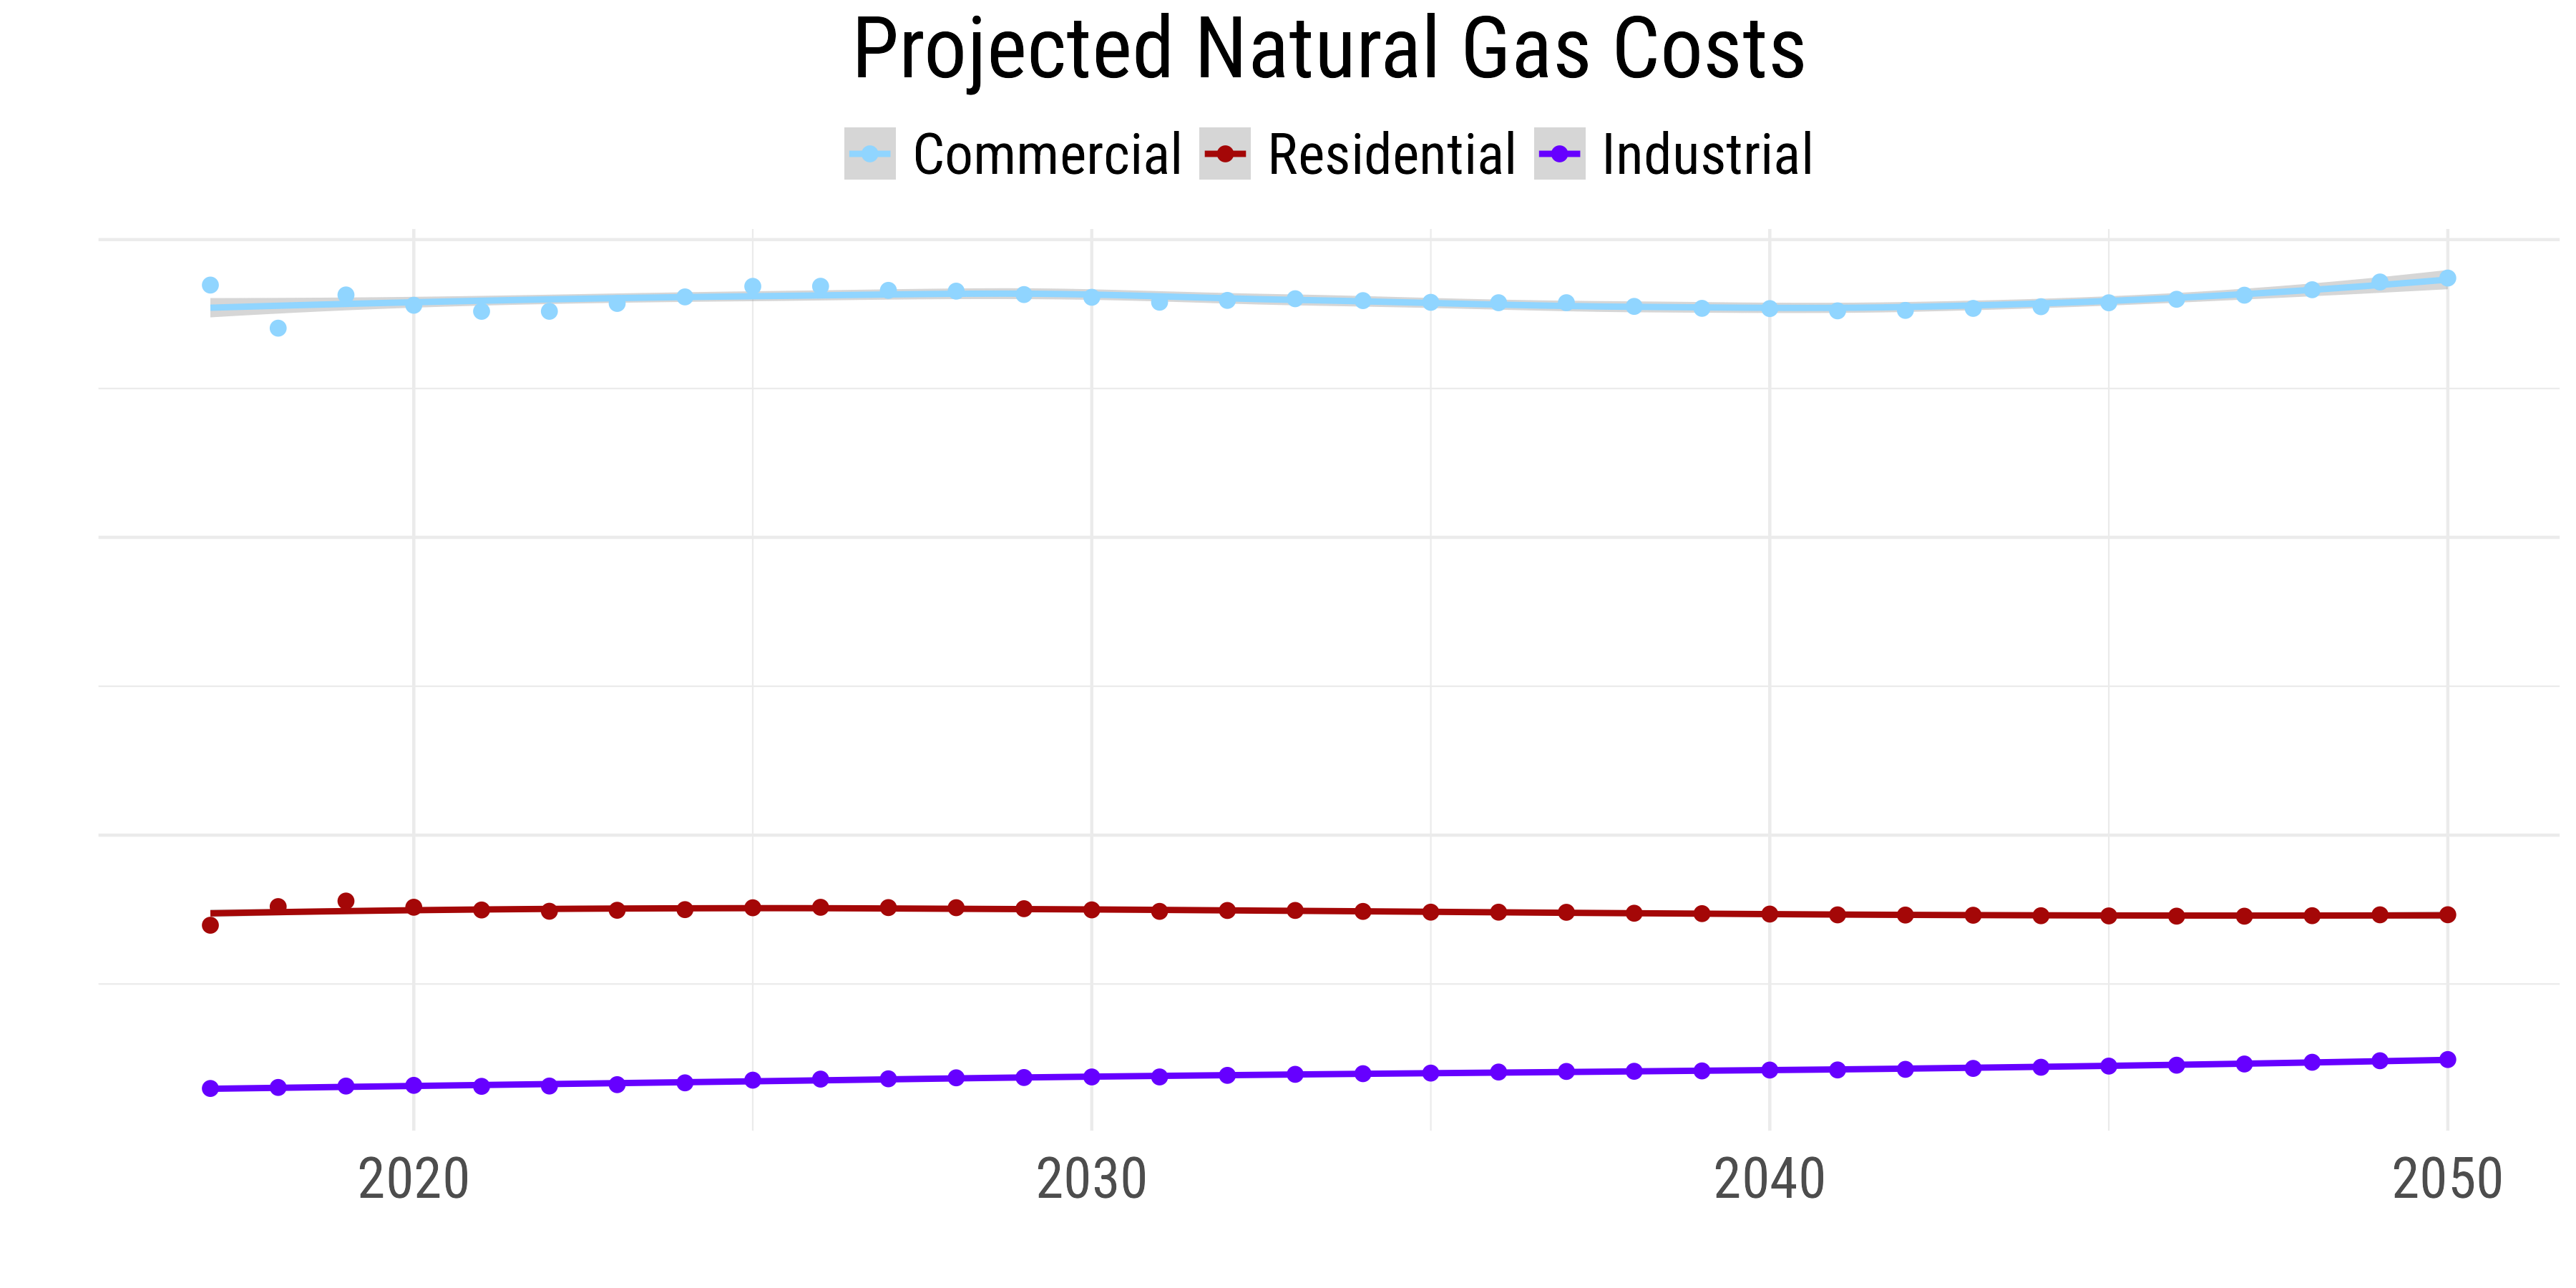
\includegraphics[width=\linewidth]{figures/energy_cost_ng.png}
     \end{subfigure}
    \rule[-5pt]{\linewidth}{0.4pt}
     \floatnote{Data come from the \href{https://maps.nrel.gov/slope/data-viewer?filters=\%5B\%5D&layer=energy-consumption.net-electricity-and-natural-gas-consumption&year=2020\&res=county}{United States Department of Energy State and Local Planning for Energy database}. All units are standardized to reflect relative, not absolute, growth and decline.}
\end{framed}
\end{figure}

\noindent Crucially, projected increase in electricity consumption and cost is likely to be driven entirely by industrial use, and to decrease in commercial and residential sectors. Overall decreases in commerical and residential energy consumption, across both sources, may be due to projected population decline across the county. If population trends reverse, expected consumption might also be projected to rise.

\subsubsection*{Renewable Resources}
\noindent \hl{[knox county has a windmill ban?]}

\pagebreak
\subsection{City Services}

\subsubsection*{Bloomfield Community Schools}

\noindent The \href{https://bloomfieldnebraska.com/education/}{City of Bloomfield Website} summarises the Bloomfield Community School District:

\begin{quote}
    Bloomfield Community School District 86R, is a Class 3 K-12 school district covering approximately 232 square miles. The elementary school and community auditorium/gymnasium were built in 1962. An addition to the elementary school was constructed in 1988 to accommodate special education, Chapter I programs and vocal music. The elementary school currently has a maximum capacity of 300. The elementary school building comprises 7,500-sq. ft. and has 19 classrooms. The auditorium/gymnasium building is 10,000-sq. ft. and also contains the vocational classrooms and shop areas. Vocational courses are currently offered at the high school level in the areas of industrial arts, agribusiness, home economics, and business. The high school also offers general education programs for adults, as well as a variety of special interest courses offered in cooperation with Northeast Community College in Norfolk and Wayne State College in Wayne. Graduate courses from Wayne State College and undergraduate courses from Northeast Community College are available.\\

    The Jr.-Sr. High School was built in 1927 and has been remodeled and updated several times. This building also has a maximum capacity of 300 and overall comprises 10,000-sq. ft. in the main building with 21 classrooms. A recent addition to the district was the installation of Distance Learning Technology over DS3 Fiber. The district has a student computer ratio of 1:4. Both the elementary and high school have a computer lab.
\end{quote}

\pagebreak
\subsubsection*{Public Lands, Buildings, and Services}

\noindent The City of Bloomfield owns multiple facilities that improve the quality of life for residents. The \href{https://bloomfieldnebraska.com/our-community/}{City of Bloomfield website} describes these facilities:

\subsubsection*{Ambulance Service}

\begin{quote}
    Established in 1969, the Bloomfield Ambulance Service is one of two ALS (Advanced Life Service) services in the county responding in the city of Bloomfield and the Bloomfield Fire District with the Bloomfield Fire Department. There are 18 state certified volunteer members of the department that include drivers, EMRs, EMTs, Paramedics and RNs with one full-time Paramedic. The department has monthly meetings/trainings and attend regularly scheduled county wide trainings. There is one ambulance in Bloomfield and one ambulance in Lindy, both of which are fully functional ALS ambulances carrying several medications, airway, trauma and 12 lead/defibrillation capable heart monitors.
\end{quote}

\subsubsection*{Fire Department}

\begin{quote}
    The City of Bloomfield Fire Department and Bloomfield Rural Fire Department operate as a volunteer organization with 35 members. The service area includes the City of Bloomfield and the surrounding rural fire district area consisting of approximately 342 square miles. On-going training and mutual aid coordination is handled at regular monthly meetings, with special training sessions provided several times each year. The fire trucks are in excellent condition and are well-equipped. The “jaws-of-life” is provided and operated by the Bloomfield Fire Department, which works in conjunction with the Bloomfield Ambulance Service. A thermal imaging camera, 1,800-gallon tanker, and a recent renovation to the fire hall enable the department to provide excellent service to the area.
\end{quote}

\subsubsection*{Police Department}

\begin{quote}
    The City of Bloomfield has a chief of police and one officer who have jurisdiction within the City and on all City property. The department provides full-time service. Communication and dispatching is through the Sheriff’s Office 911 system. The Knox County Sheriff’s Office, Nebraska State Patrol, Nebraska Game \& Parks, and Nebraska Fire Marshall also have jurisdiction.
\end{quote}

\subsubsection*{Community Center/City Hall}

\begin{quote}
    The Community Center and City Hall are located near the center of the business district. Built in 1995, this masonry structure is in excellent condition and is in compliance with ADA requirements. The building houses the city administrator’s office, clerk’s office, police department, and council chambers. The facility also offers a community room, which is utilized by various civic organizations including the senior citizens group for regular meetings and special events, such as potluck dinners. The city clerk’s office handles the reservations for the use of the community room.  The council room is also available for smaller groups. The American Legion Pavilion is also available for reservations. The American Legion Pavilion has air-conditioning and tables and chairs are included in reservation. The American Legion Pavilion now has an in-house speaker system for speaking and to play music through via Ipods and CDs.
\end{quote}

\subsubsection*{Library}

\begin{quote}
    The Bloomfield Public Library was organized in 1908. The Bloomfield Library Foundation completed a new public library building in 2000. The building houses the Bloomfield Public Library and Learning Center. High speed internet access is available on a number of public computers. The latest effort to boost technology includes participation in Library Broadband Builds Nebraska Communities, a project through the Nebraska Library Commission. Books, videos, cake pans, puzzles, puppets and cassette tapes are all available at the library.
\end{quote}

\pagebreak
\subsubsection*{Parks and Recreation}

\noindent The City of Bloomfield has two parks, a swimming pool, and the Knox County Fairgrounds. The \href{https://bloomfieldnebraska.com/our-recreation/}{City of Bloomfield website} describes several of them:

\subsubsection*{City Parks}
\begin{quote}
    The City of Bloomfield has two parks. The “City Park” is located in the south central part of the city. This park features a picnic shelter, horseshoe pits, two basketball hoops with concrete pads,  and restrooms.  The city park became home to new playground equipment in 2006. The second park is the “Robin Schulz Memorial Park.” This park is located in the north part of the city. The park features a lighted regulation size softball field with enclosed dugouts, sheltered bleachers, restrooms, equipment rooms, and a concession stand. A second softball field, added in 1997, features enclosed dugouts and a ground level pressbox.
\end{quote}

\subsubsection*{Swimming Pool}
\begin{quote}
    The municipal outdoor heated swimming pool was built in 1977, with a number of equipment replacements and upgrades since 1993, including the addition of a handicap accessibility lift system in 1994. The pool is located in the south central part of the city and is open from early June to early August. A picnic area with shelter is located adjacent to the swimming pool. A new slide and basketball hoop were added in 2000.
\end{quote}

\subsubsection*{Fairgrounds}
\begin{quote}
    The Knox County Fairgrounds, owned by the city, are located on the eastern edge of Bloomfield.  The fairgrounds contain a rodeo arena and livestock boarding, exhibition buildings, and camping spots with electrical outlets. In addition to the traditional buildings, the fairgrounds features a lighted baseball field with a concrete grandstand, restrooms, ticketbooth, and concession stand. Other features include a lighted football field.
\end{quote}

\pagebreak
\noindent Bloomfield residents have mixed evaluations of these facilities. \textbf{Figure~\ref{fig:scoreParks}} shows that they have positive evaluations of the fairgrounds and Robin Schulz Memorial Park, but neutral to negative evaluations of the Swimming Pool and City Park.

\begin{figure}[H]
\centering
\begin{framed}
    \caption{Community Assessment of Public Parks and Recreation}
    \label{fig:scoreParks}
    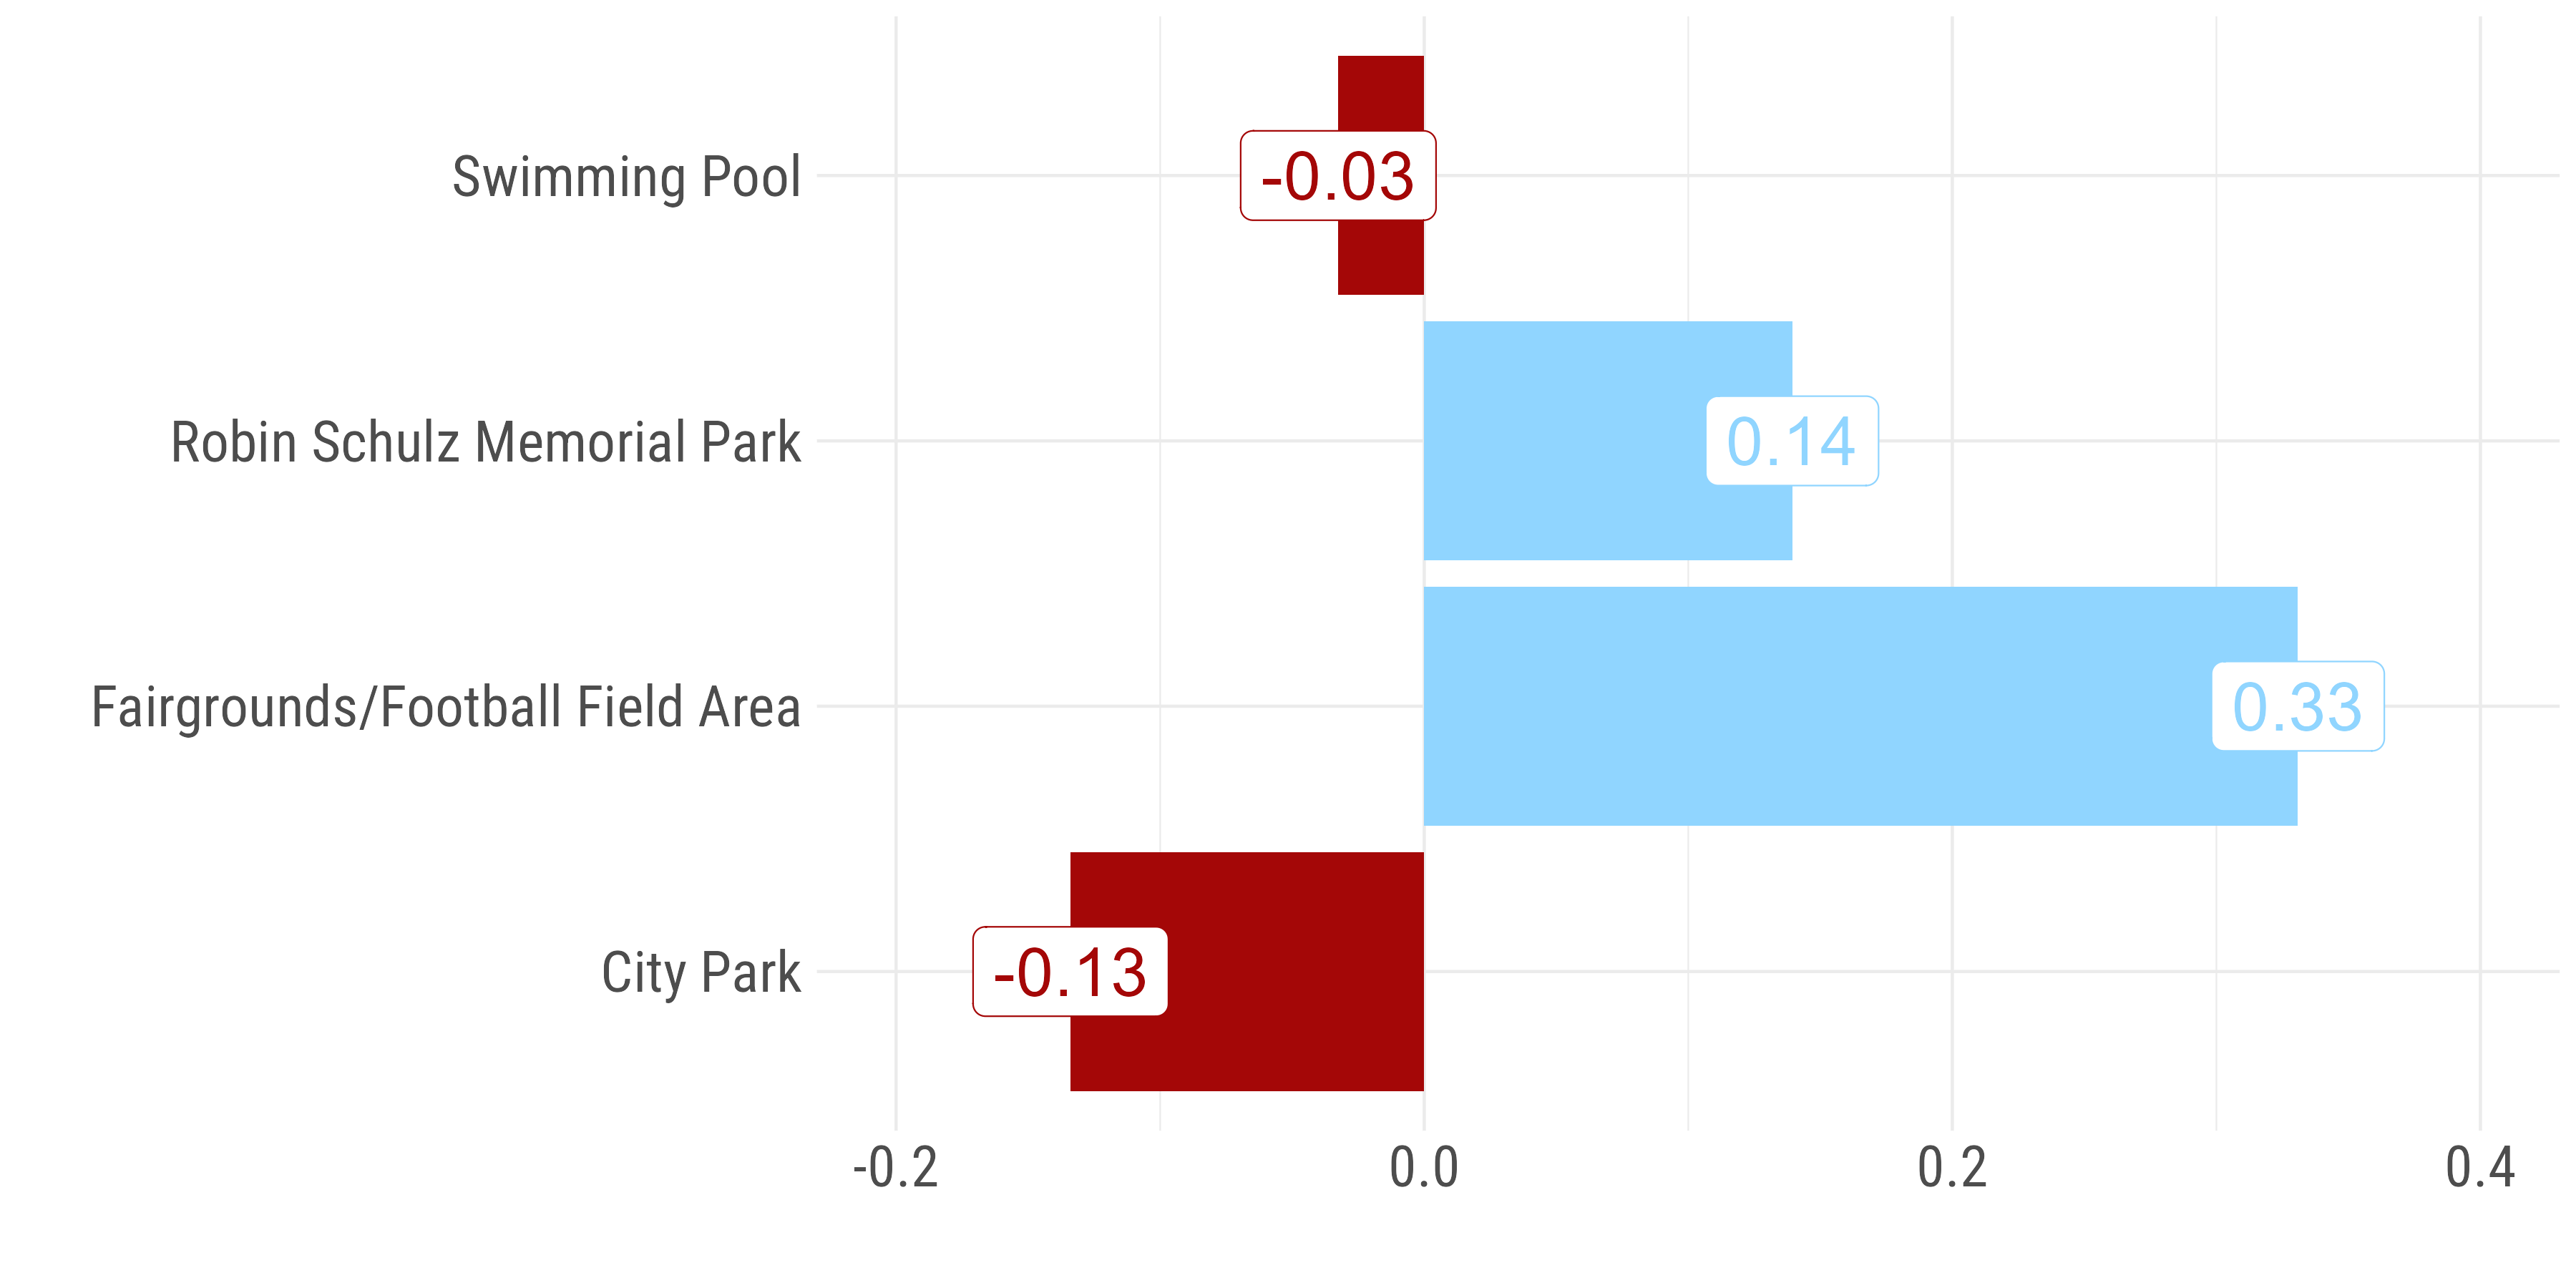
\includegraphics[width = \linewidth]{figures/score_parks.png}
\end{framed}
\end{figure}

\pagebreak
\subsubsection*{Bloomfield Municipal Airport}

\noindent \hl{[Is the airport owned by the city? I thought it was privately owned]}

\pagebreak
\subsection*{Key Takeaways}
\pagebreak
\section{Future Land Use}

\noindent \hl{[do more to fully introduce this section]}\\

\noindent Maps on the following pages are the proposed future land use (FLU) maps for Bloomfield's entire zoning jurisdiction. They should guide all land use and development decisions over the next ten years. Should the Bloomfield Planning Commission and the City Council choose to make policy decisions that are not reflected on the FLU map, then the FLU map must be amended to reflect the change in policies.

\thispagestyle{empty}
\begin{landscape}
    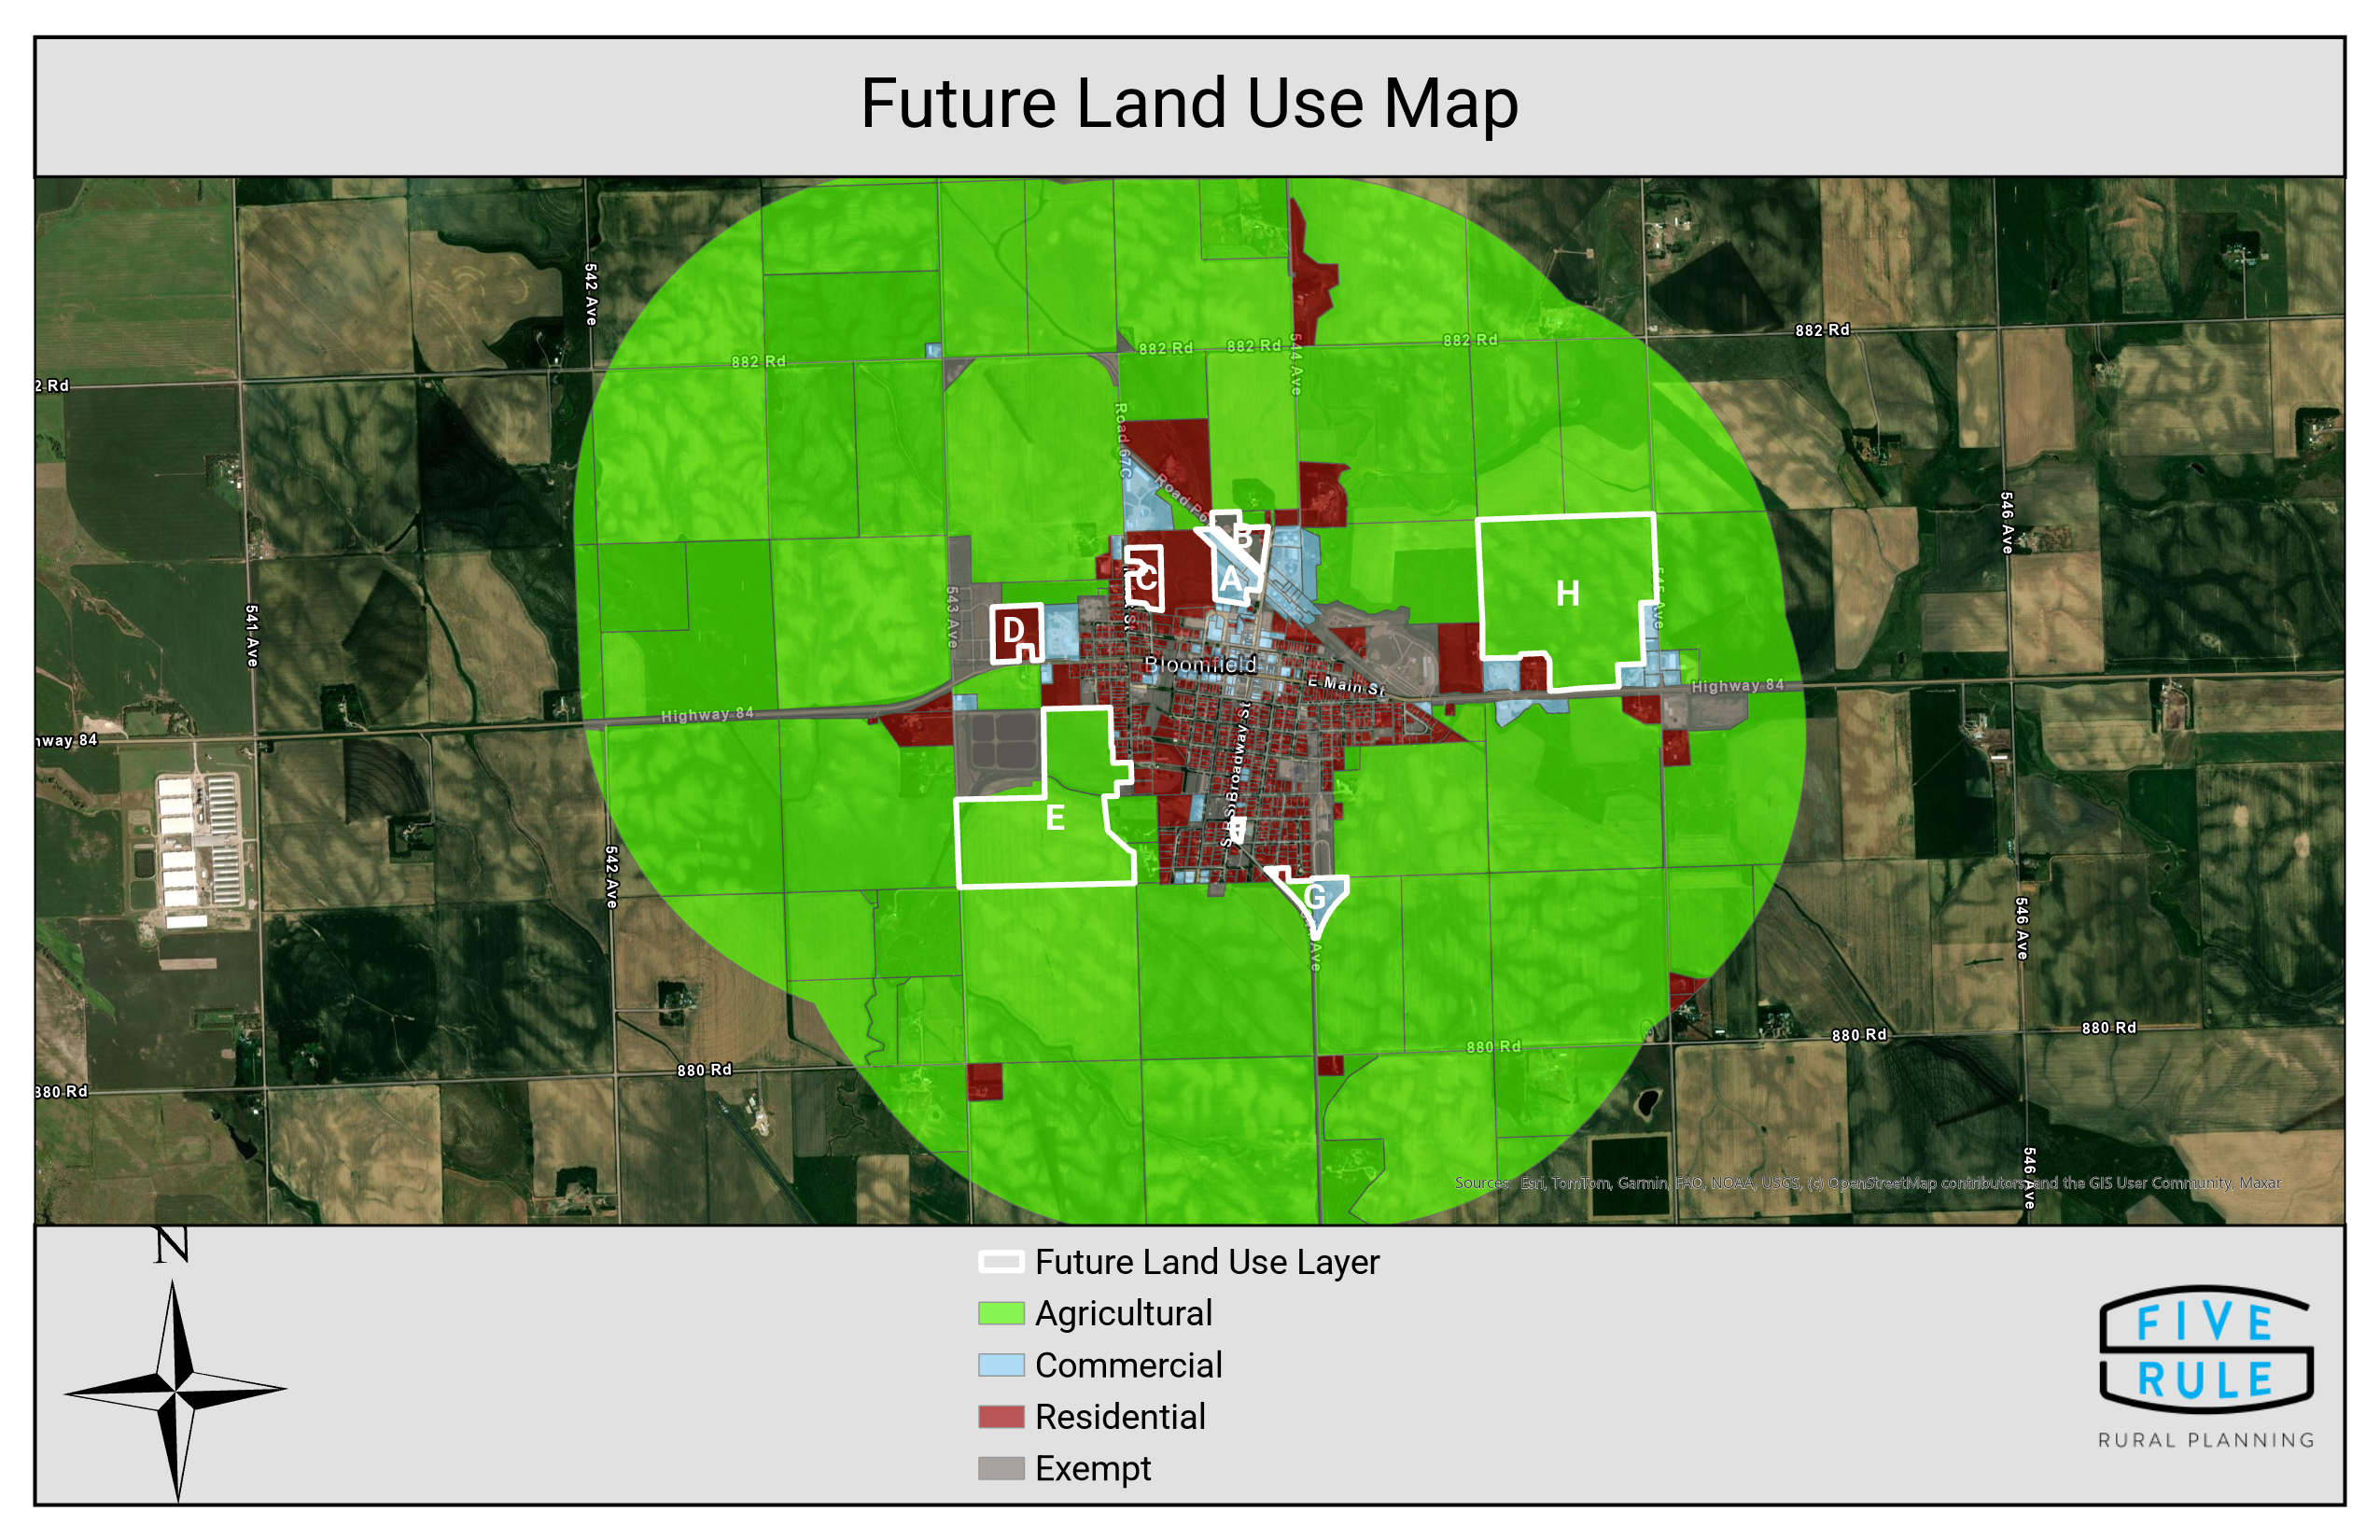
\includepdf[angle = 90]{maps/flu_all.pdf}
\end{landscape}

\pagebreak
\thispagestyle{empty}
\begin{landscape}
    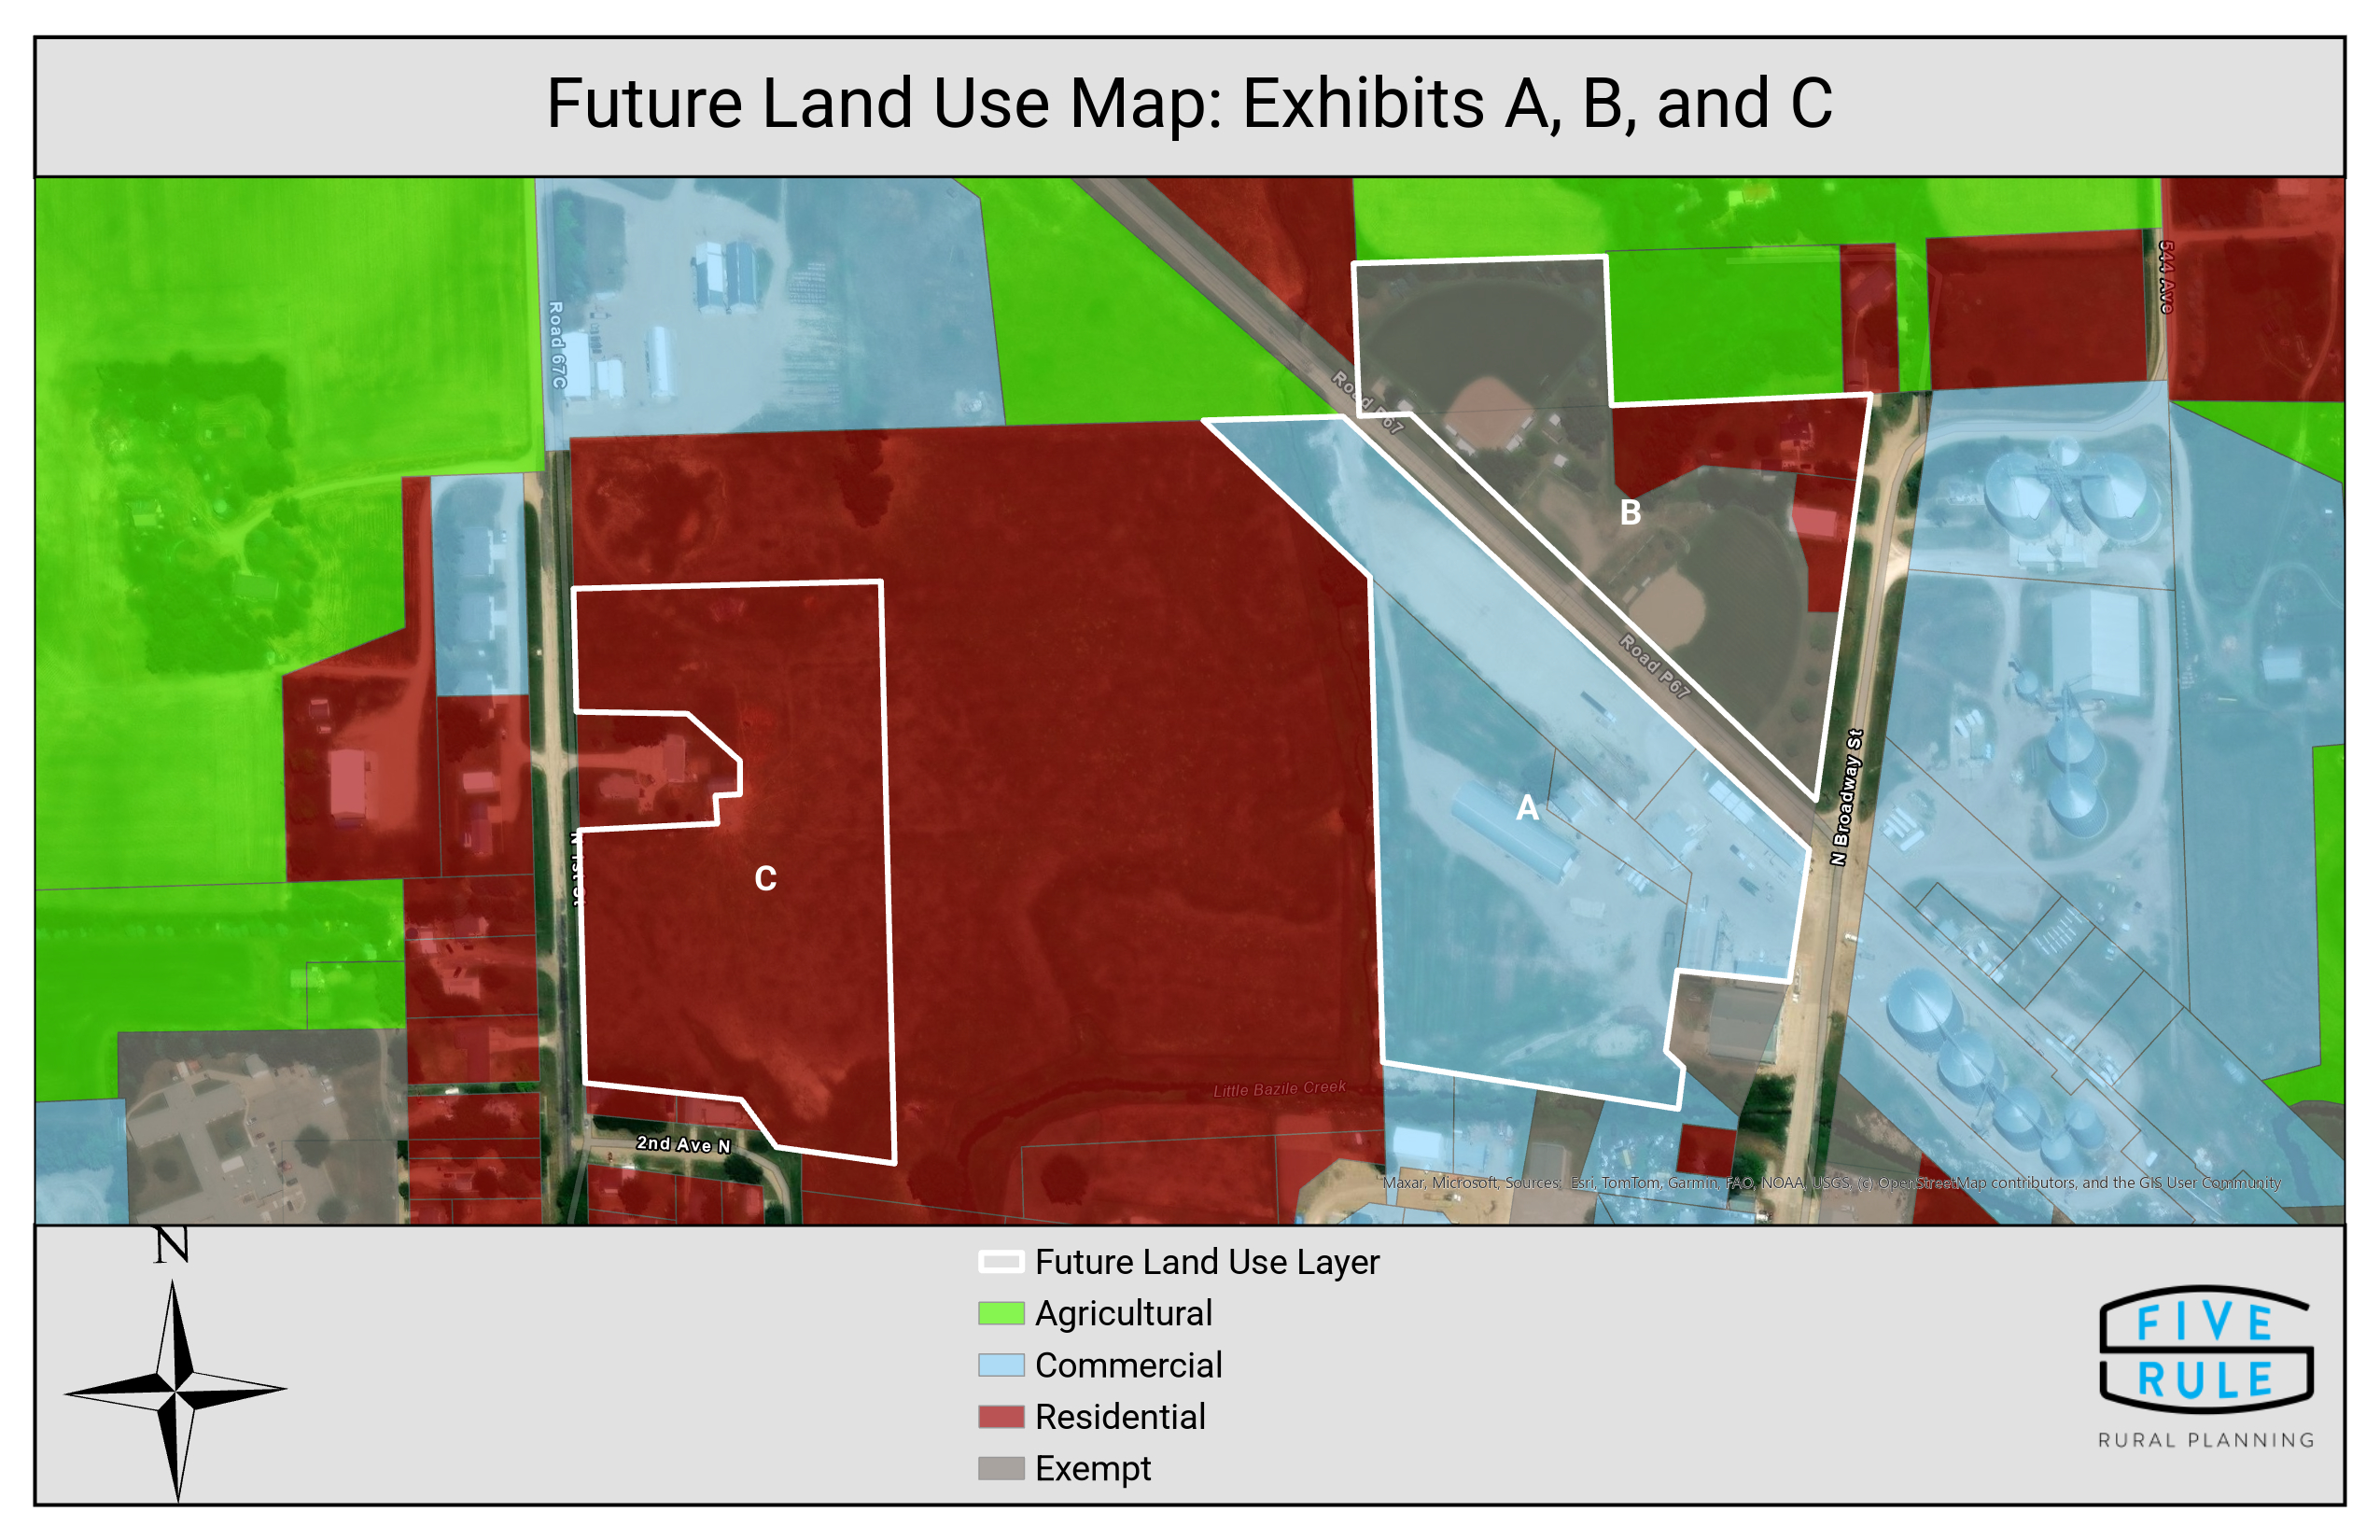
\includepdf[angle = 90]{maps/flu_abc.pdf}
\end{landscape}

\pagebreak
\thispagestyle{empty}
\begin{landscape}
    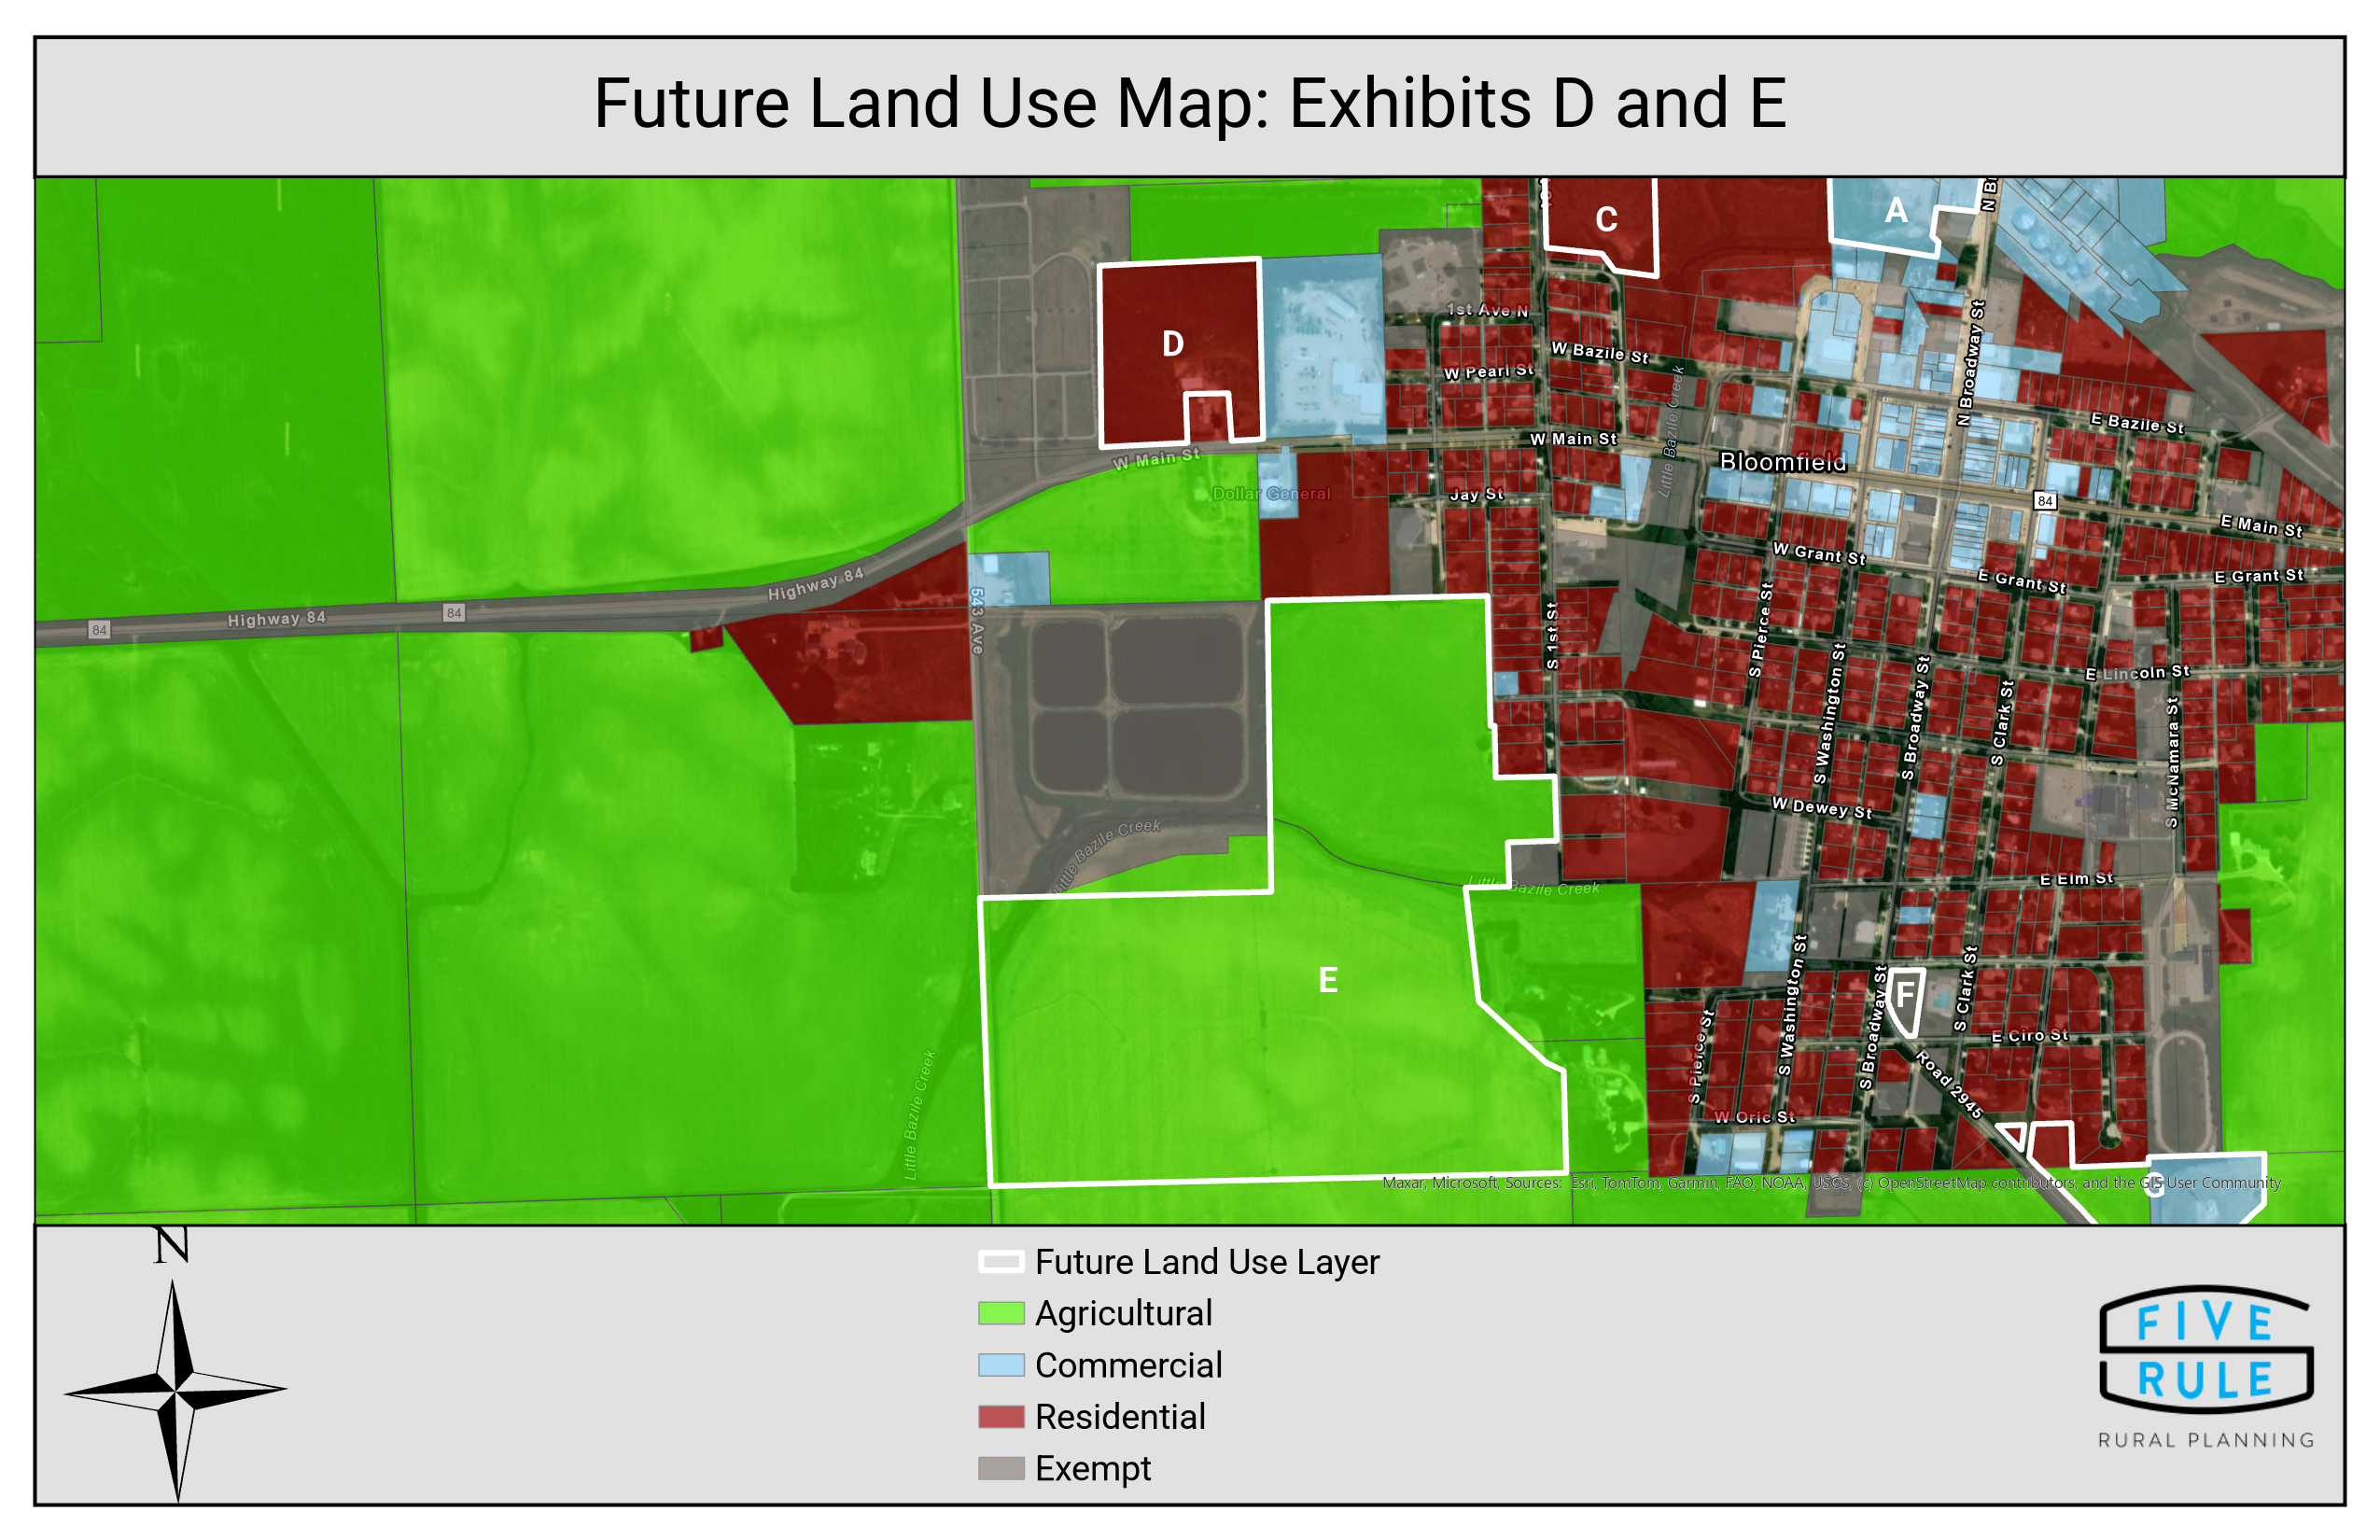
\includepdf[angle = 90]{maps/flu_de.pdf}
\end{landscape}

\pagebreak
\thispagestyle{empty}
\begin{landscape}
    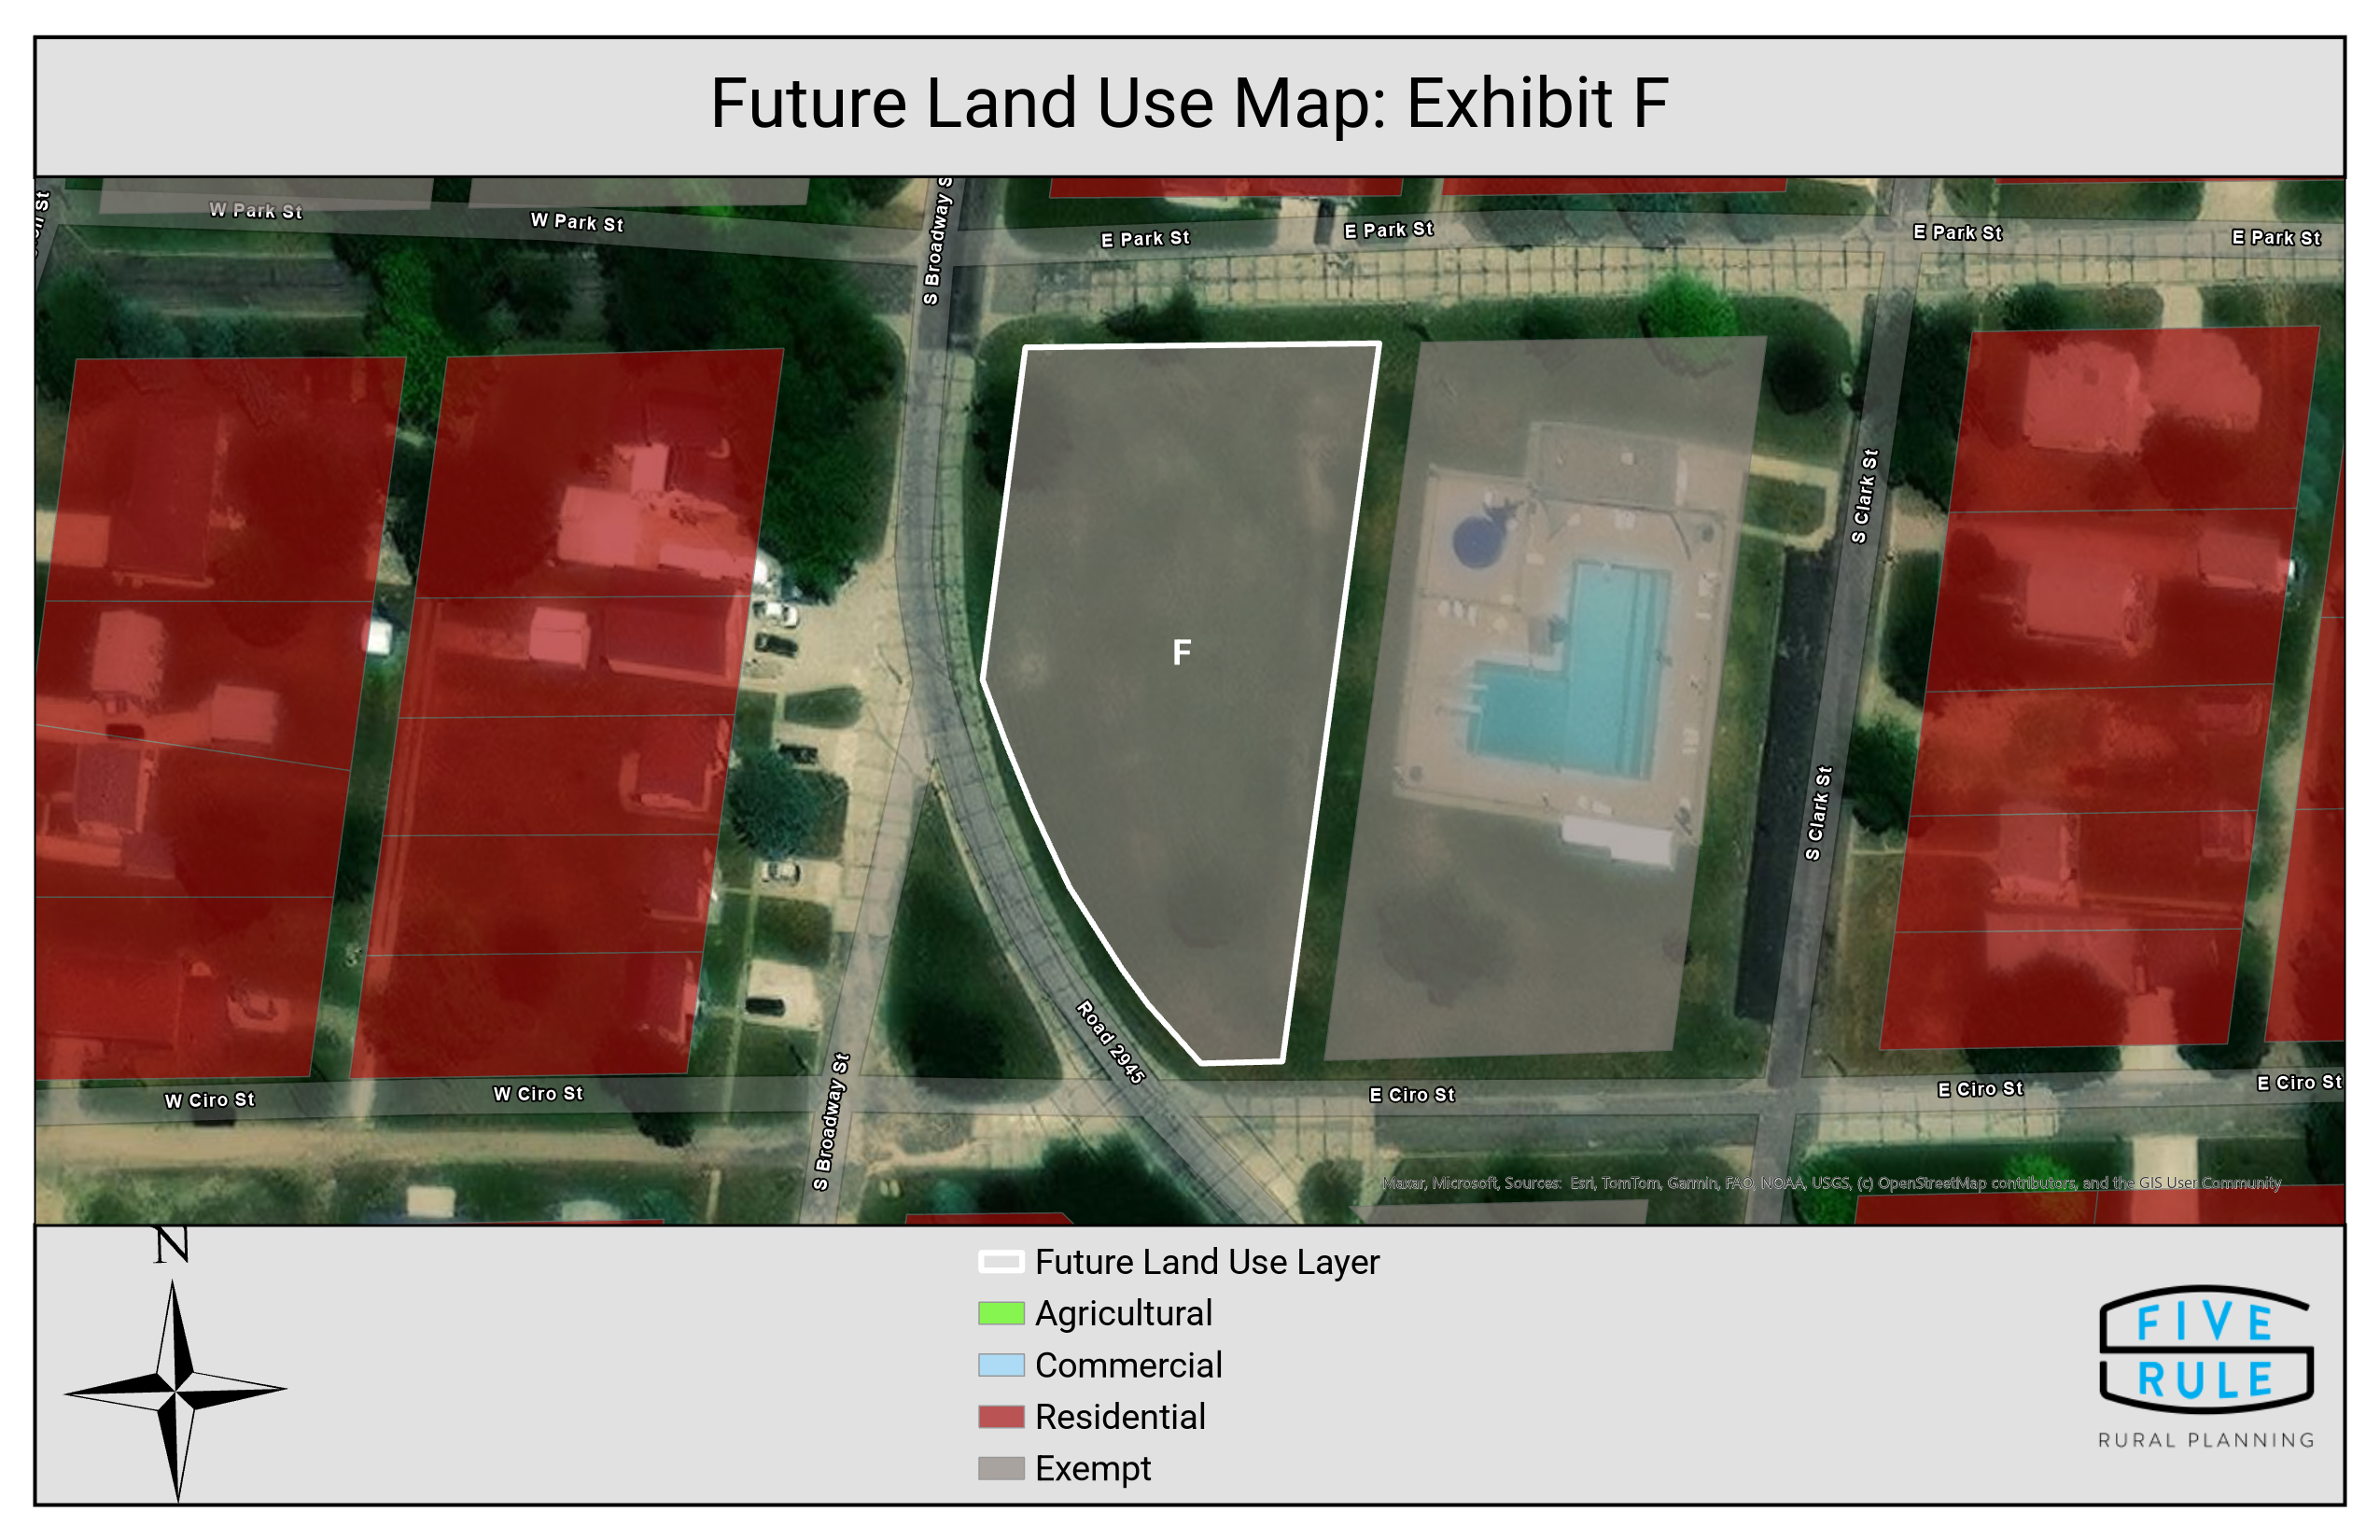
\includepdf[angle = 90]{maps/flu_f.pdf}
\end{landscape}

\pagebreak
\thispagestyle{empty}
\begin{landscape}
    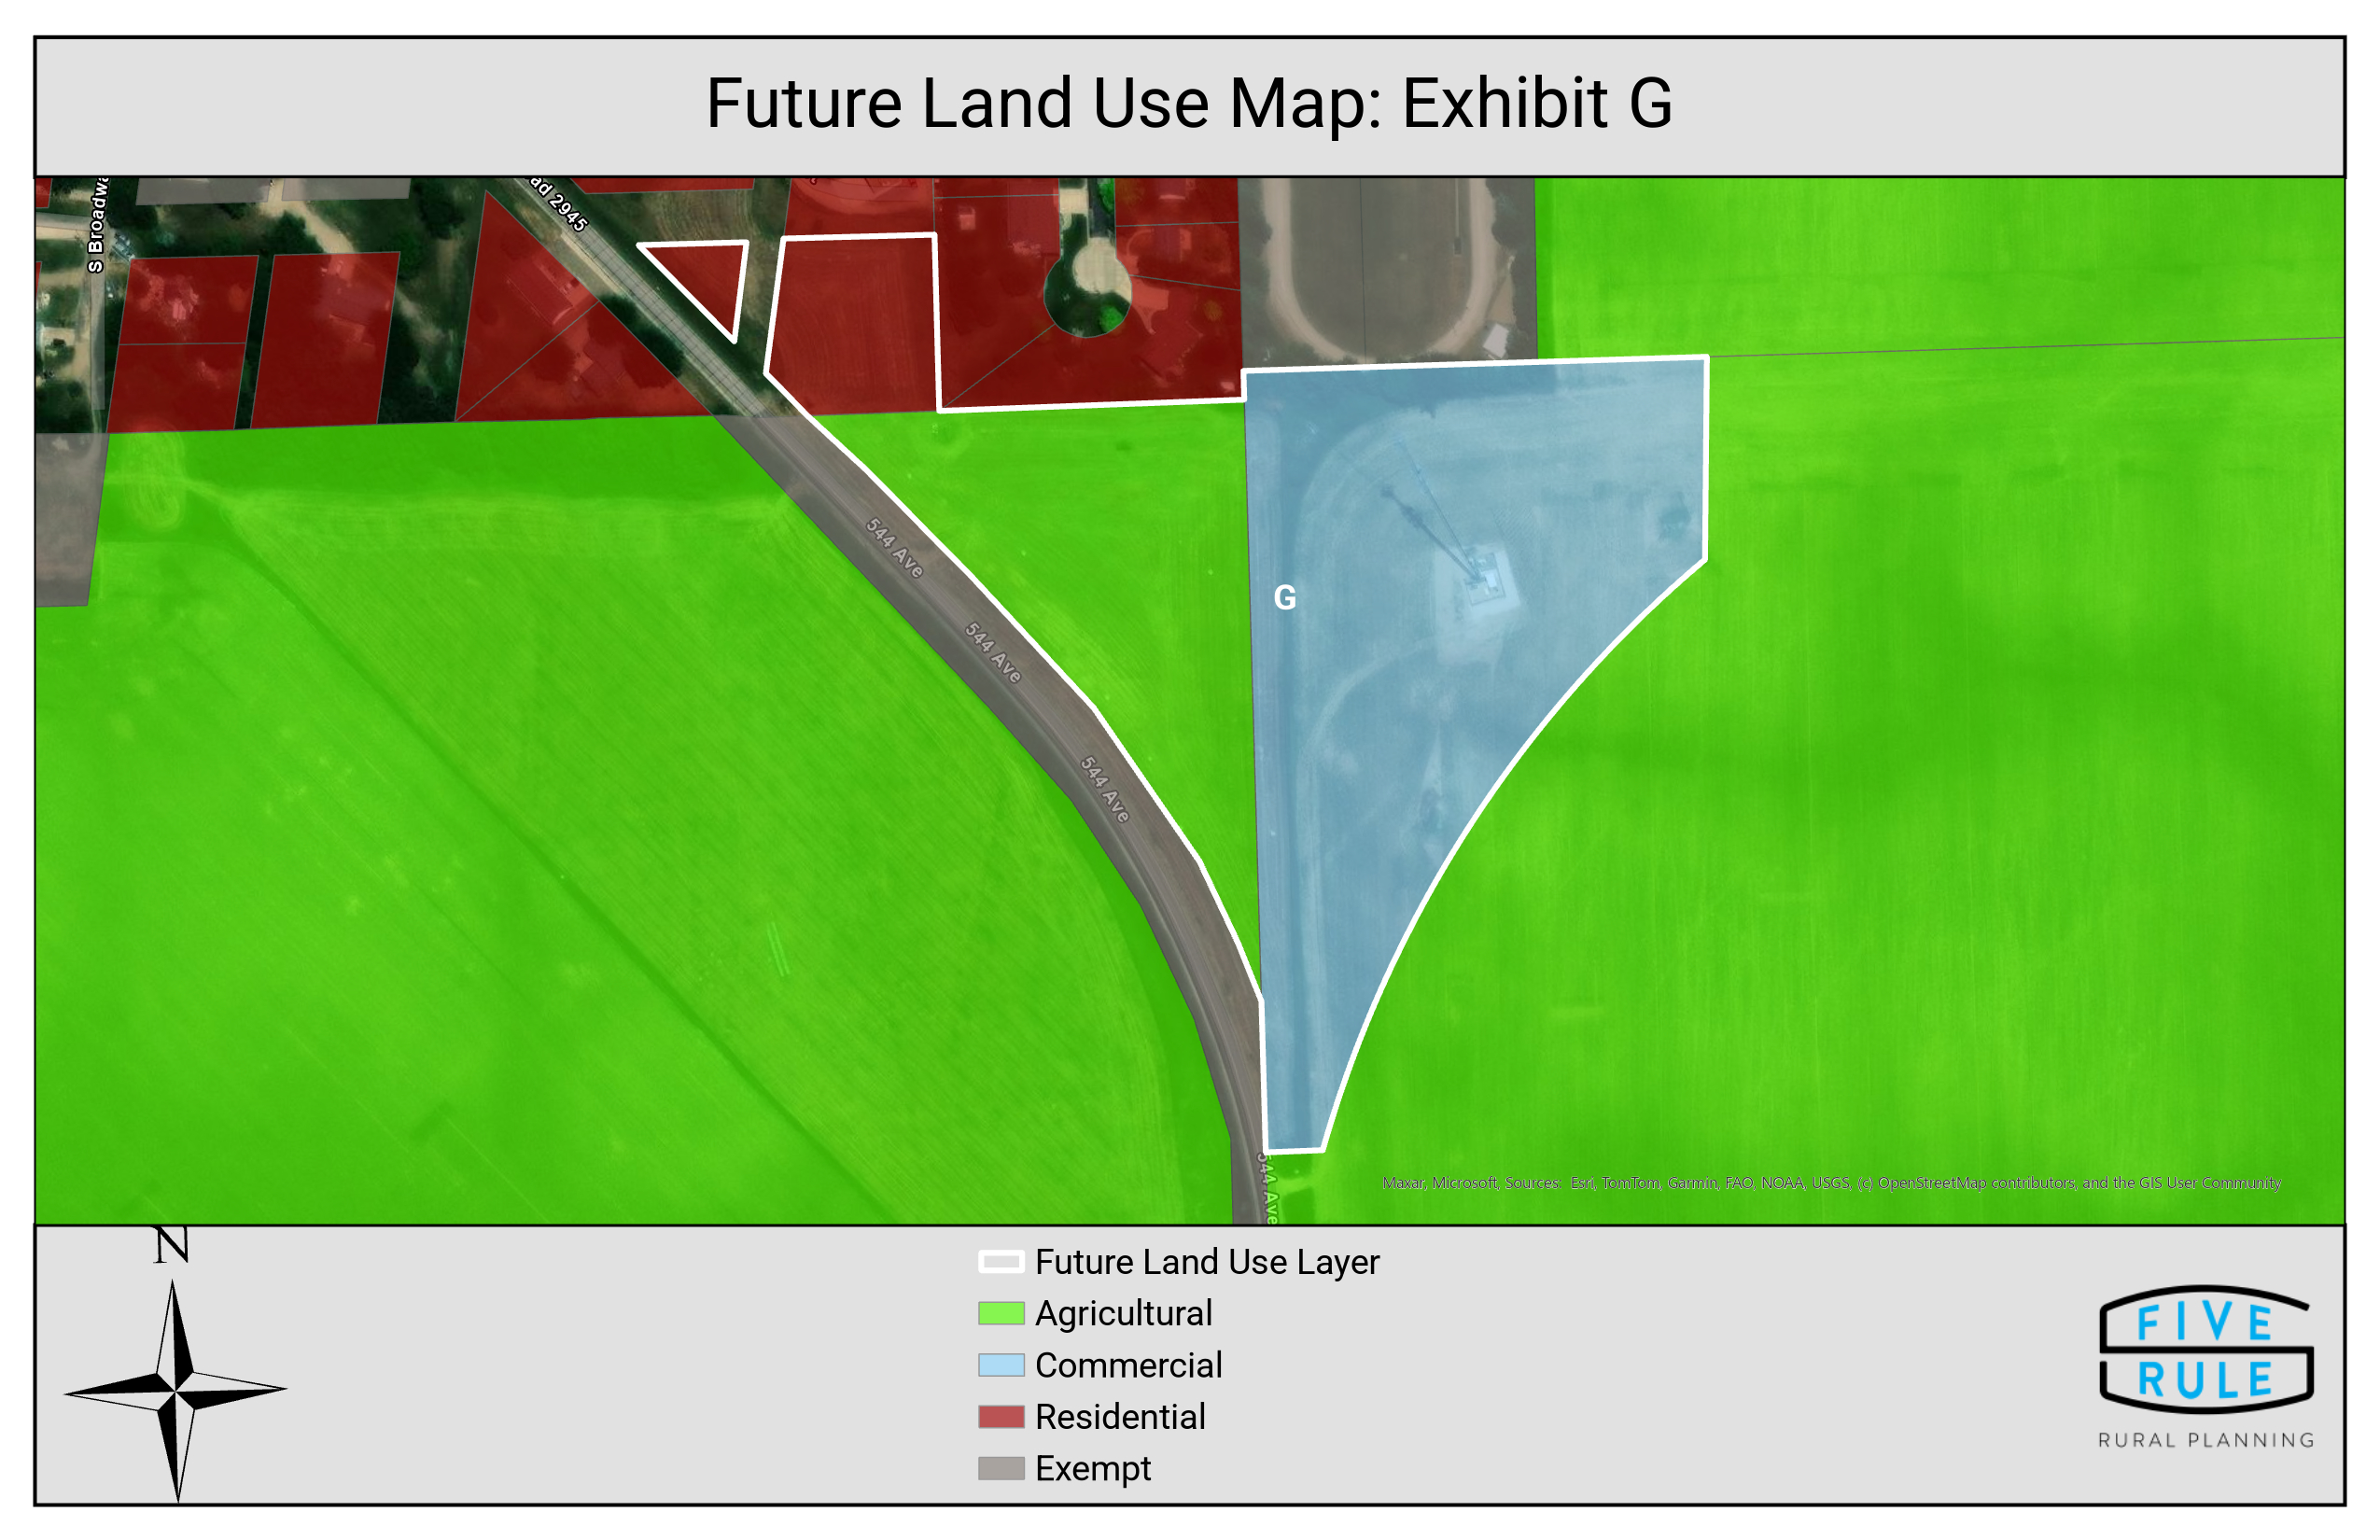
\includepdf[angle = 90]{maps/flu_g.pdf}
\end{landscape}

\pagebreak
\thispagestyle{empty}
\begin{landscape}
    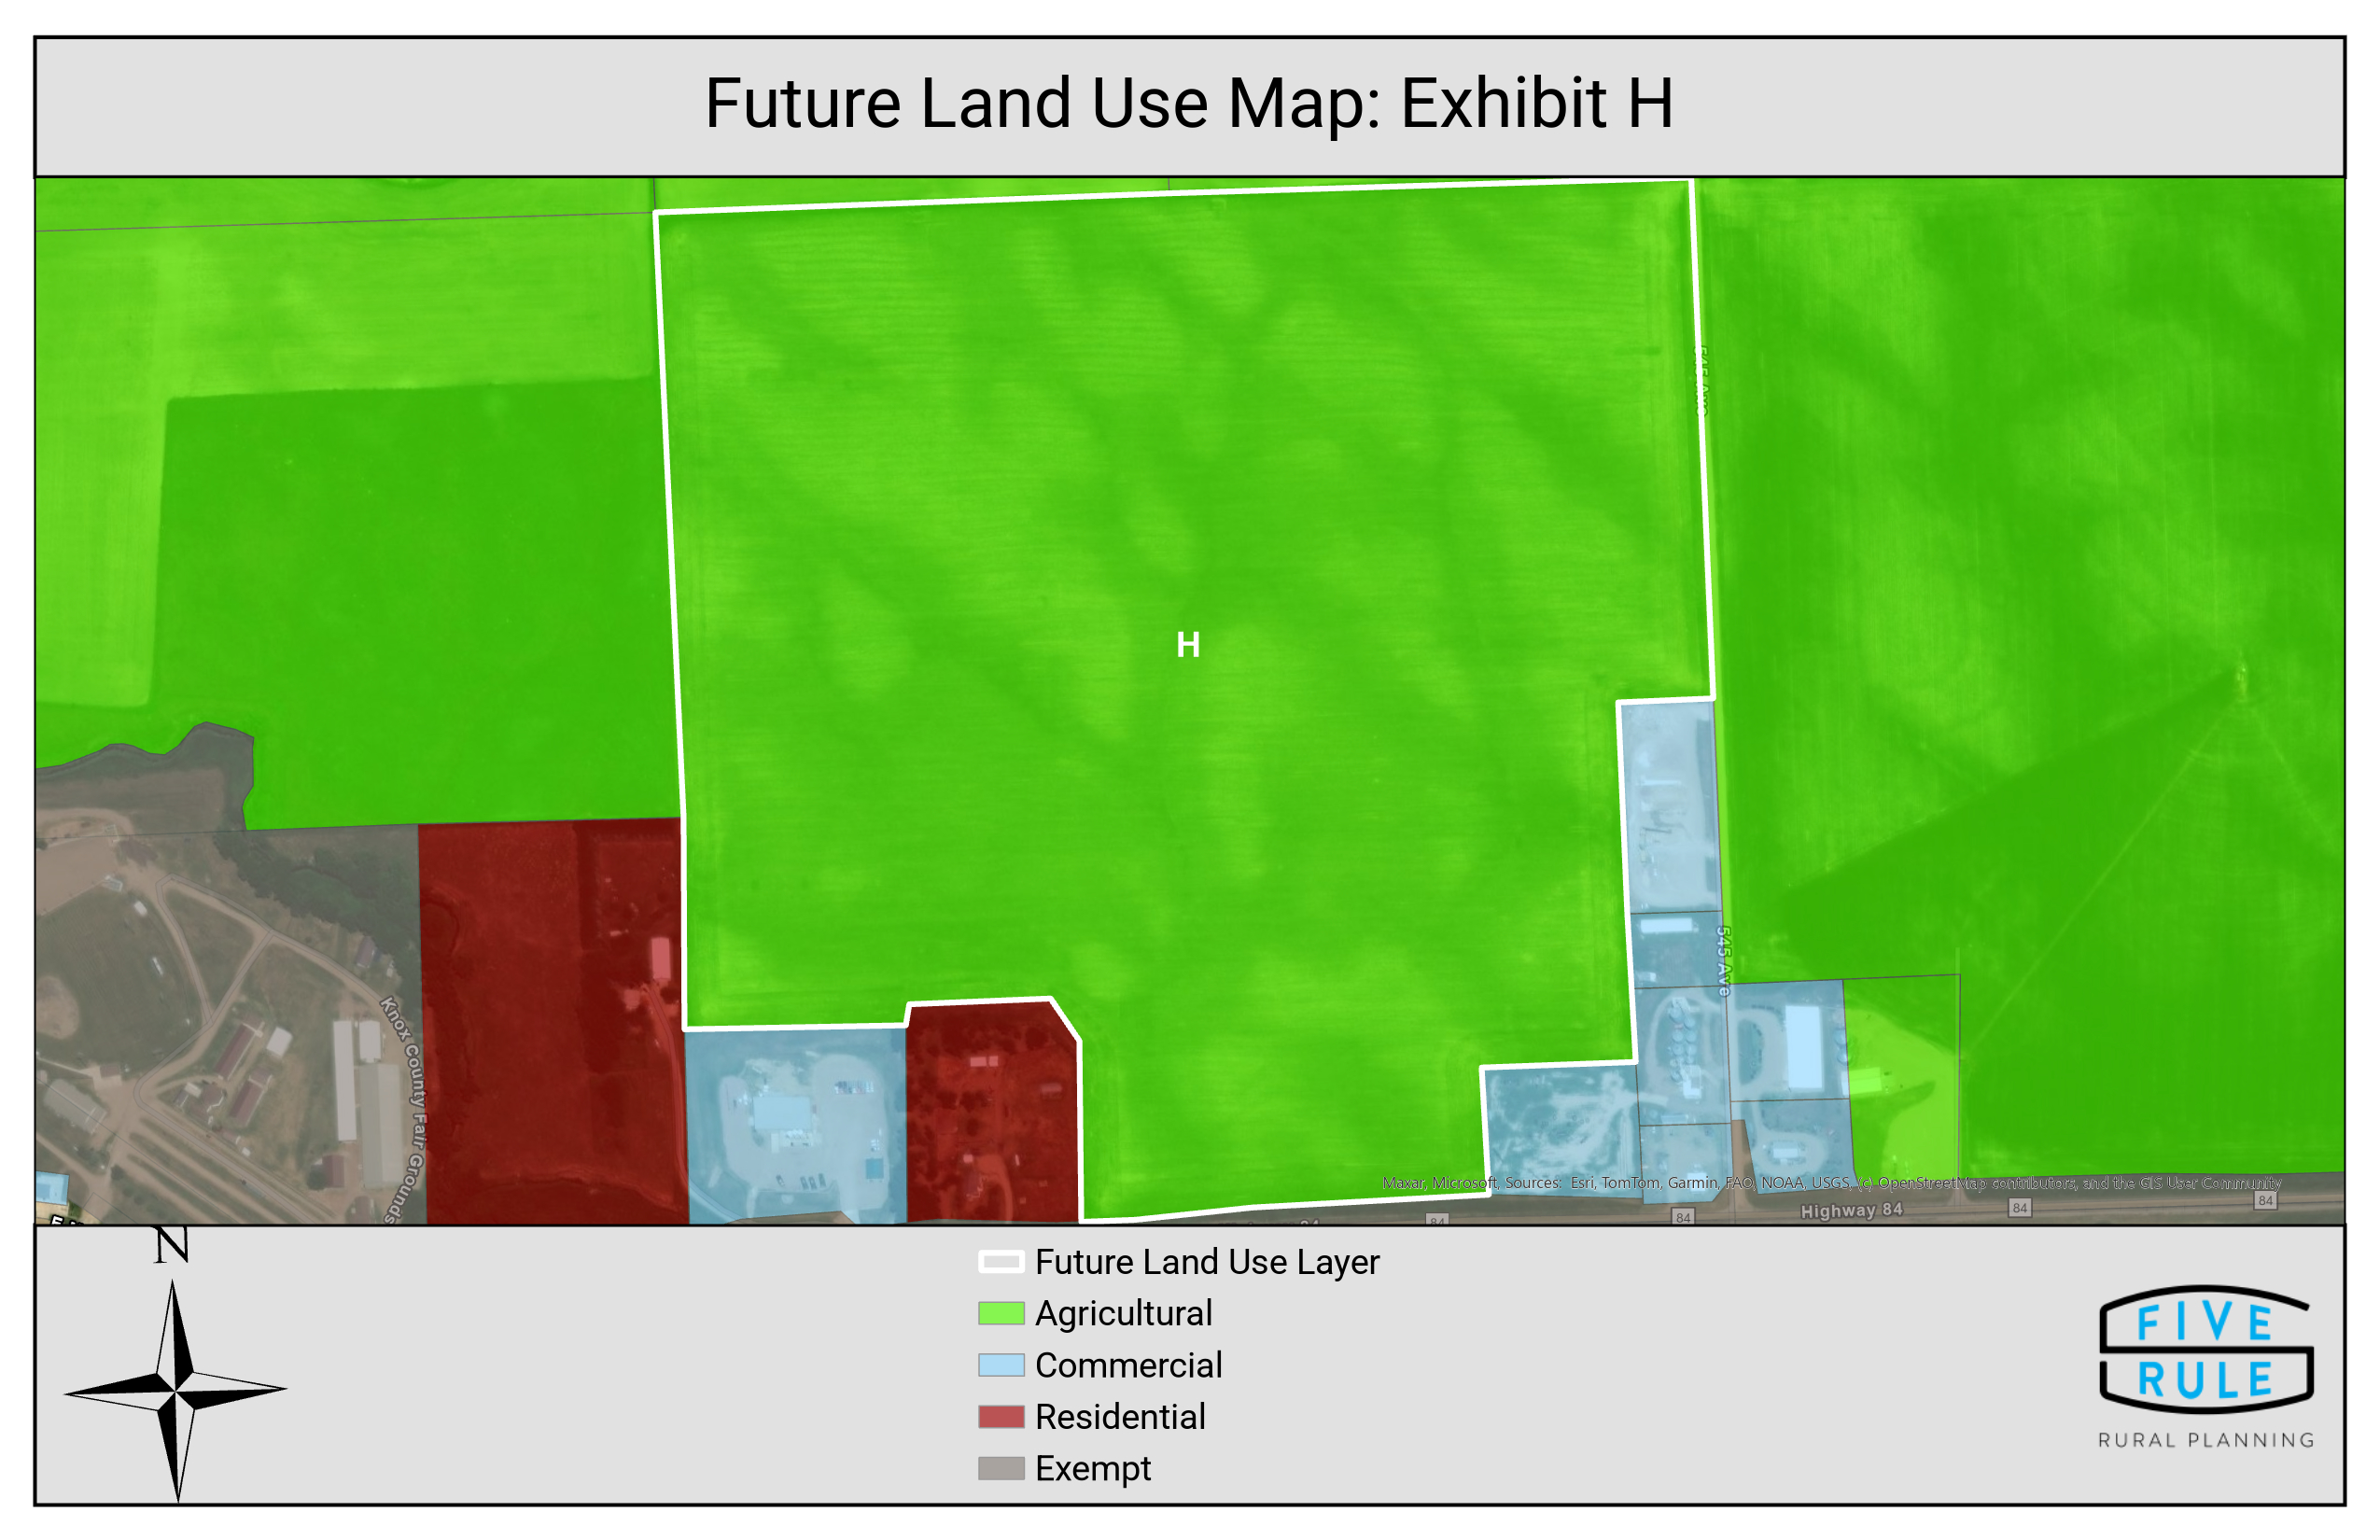
\includepdf[angle = 90]{maps/flu_h.pdf}
\end{landscape}

\pagebreak
\subsection{Description of Future Land Use Exhibits}

\noindent \hl{[i would love to follow up with the Bloomfield folks on this at some point]}

\subsubsection*{Exhibit A}

\noindent Expansion of the Farmers Pride Cooperative, currently listed as commercial land use.

\subsubsection*{Exhibit B}

\noindent Addition of a concessions stand and renovations to softball fields at Robin Schulz Memorial Park.

\subsubsection*{Exhibit C}

\noindent New residential development off of N 1st street, currently listed as residential land use.

\subsubsection*{Exhibit D}

\noindent New residential development east of the Bloomfield Cemetery, currently listed as residential land use.

\subsubsection*{Exhibit E}

\noindent New residential development south of the Dollar General and west of the Good Samaritan Society-Sunset View Assisted Living facility, currently listed as agricultural land use

\subsubsection*{Exhibit F}

\noindent Lands to the west of the swimming pool may be suitable for a new pickleball court or other source of recreation.

\subsubsection*{Exhibit G}

\noindent New residential development along South Broadway street exiting/entering Bloomfield, currently listed as a combination of residential, commercial, and agricultural land use.

\subsubsection*{Exhibit H}

\noindent New expansion of industrial development east of Bloomfield, currently listed as agricultural land use.
% \pagebreak
% \input{pages/07_energy}

\pagebreak
\appendix
\section*{Appendix}

\noindent There are three kinds of data used to generate this \textbf{\textcolor{coBalt}{Comprehensive Development Plan}}: community engagement data, socioeconomic data, and map and geospatial data. This appendix documents how these data were acquired, processed, and presented. Finally, it also summarizes the technical procedures used to generate the tangible document of the plan.

\section{Community Engagment Process}

\noindent Community and resident engagement is crucial to the Plan for several reasons:
\begin{enumerate}
    \item [(1)] \textbf{Inclusivity and Representation}: The Plan intends to address the needs and aspirations of the entire community. Including as many residents as possible ensures that a diverse range of voices and perspectives are heard and considered. This helps with efforts to reflect the values, priorities, and aspirations of the whole community.
    \item [(2)] \textbf{Local Knowledge and Expertise}: Local knowledge and input help to ground the Plan in the realities of the area. Residents have firsthand knowledge about their neighborhood and its unique characteristics. Their insights are invaluable to identifying specific needs and opportunities that would only be known by those who experience Bloomfield daily.
    \item [(3)] \textbf{Trust and Transparency}: Engaging residents in the planning process builds trust between the community and the municipal government. Transparent and inclusive decision-making processes foster greater confidence that the plan is responsive to community needs. This trust will build partnerships between residents, local government, and other stakeholders necessary to implement the Plan.
\end{enumerate}

\subsection{Bloomfield Community Engagement Process}
\noindent Residents, stakeholders, and advocates were engaged on \hl{N} separate occasions throughout the entire planning process.
\begin{enumerate}
    \item [(1)] \hl{[list of engagements]}
\end{enumerate}

\subsection{Community Engagement Kickoff}

\noindent The community engagement process began with identifying and inviting local stakeholders and advocates to assist with identifying priorities early in the process. A \textbf{\textcolor{coBalt}{stakeholder}} is any resident that has a vested interest in seeing Bloomfield grow as a community. An \textbf{\textcolor{coBalt}{advocate}} is any individual involved with the community that can speak up for stakeholders who are unable to participate in the community engagement process.\\

\noindent The consultant team hosted the kickoff on \hl{[date]} to provide an overview of the planning process and invite attendants to participate in a model building and consensus workshop scheduled in November 2023.

\subsection{Model Building and Consensus Workshop}

\noindent On November 7, 2023, Bloomfield residents, stakeholders, and advocates attended a community consensus workshop facilitated by community and economic development consultants with FIVE RULE Rural Planning of Kearney, NE. Lowell Schroeder and Bobbi Pettit facilitated a conversation among roughly 50 members of the Bloomfield Community.

\subsubsection*{Model Building Introductions}
\noindent Attendees introduced themselves through an inclusive participatory process that asked each participant to remember a time when he or she felt very happy, safe, and proud to be a member of the Bloomfield Community. They were then asked to select a random found object and use that object to describe the memory. Each participant introduced themselves, described their relationship to the Bloomfield Community, and described their object and memory. Every attendee shared a positive memory.\\

\noindent The ToP Consensus Workshop Method was utilized to assist attendees with identifying themes and creating a shared vision for the next decade in Bloomfield. The group was asked \textit{“What is needed now to make Bloomfield Better?"}\\

\noindent Each participant brainstormed immediate ideas (3 to 5 words) that came to mind when asked this question and then worked together with their tablemates to sort and organize the ideas. Ideas were then combined and sorted on a shared wall. This exercise ultimately led to the themes addressed in the eventual community survey.\\

\subsection*{Workshop themes}

\noindent \hl{[insert image of workshop themes HERE]}

\subsection{Communitywide Survey}

\noindent The themes that rose to the surface because of the workshop were utilized to create a survey made available to the entire Bloomfield community \hl{[in Spring 2024]}. Survey responses are reported throughout the plan where appropriate.\\

\noindent The survey was made available in both online and paper copy formats. 162 respondents participated in the survey.

\begin{figure}[ht!]
\centering
\begin{framed}
    \caption{Community Survey Neighborhoods}
    \label{fig:neighborhoods}

     \begin{subfigure}{0.49\textwidth}
        \centering
        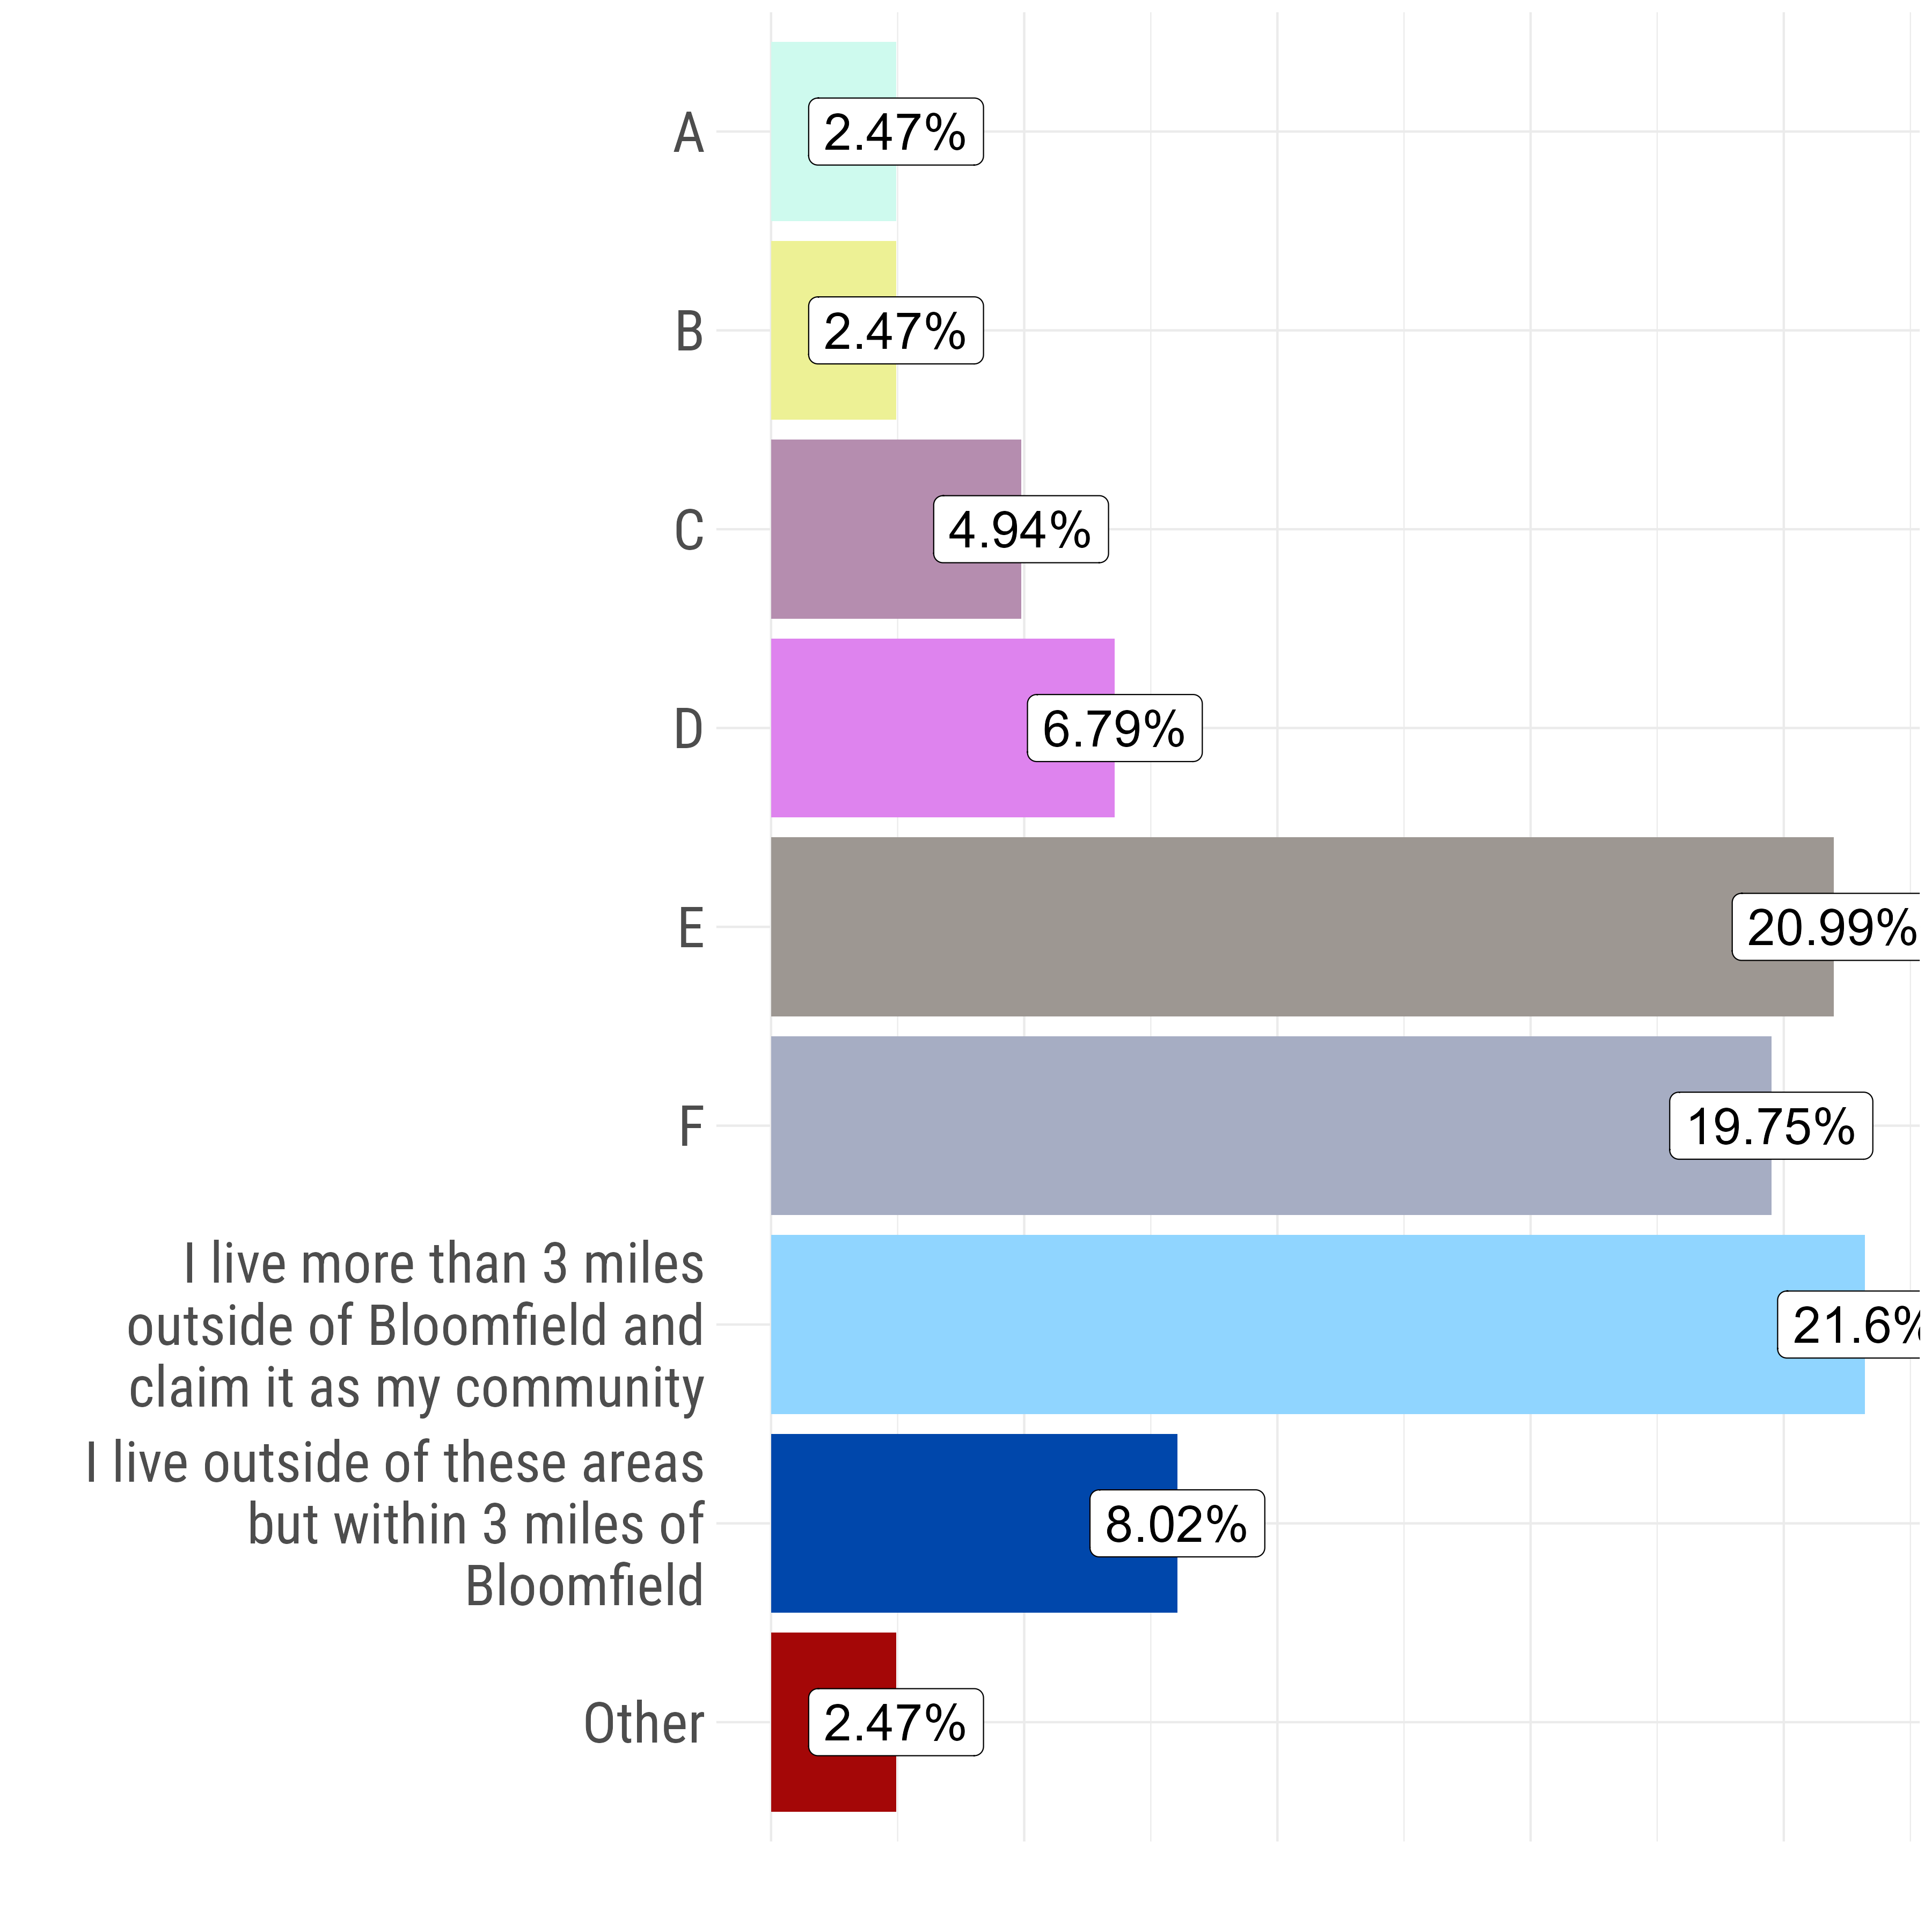
\includegraphics[width=\linewidth]{figures/survey_respondent_neighborhoods.png}
     \end{subfigure}
     \begin{subfigure}{0.49\textwidth}
        \centering
        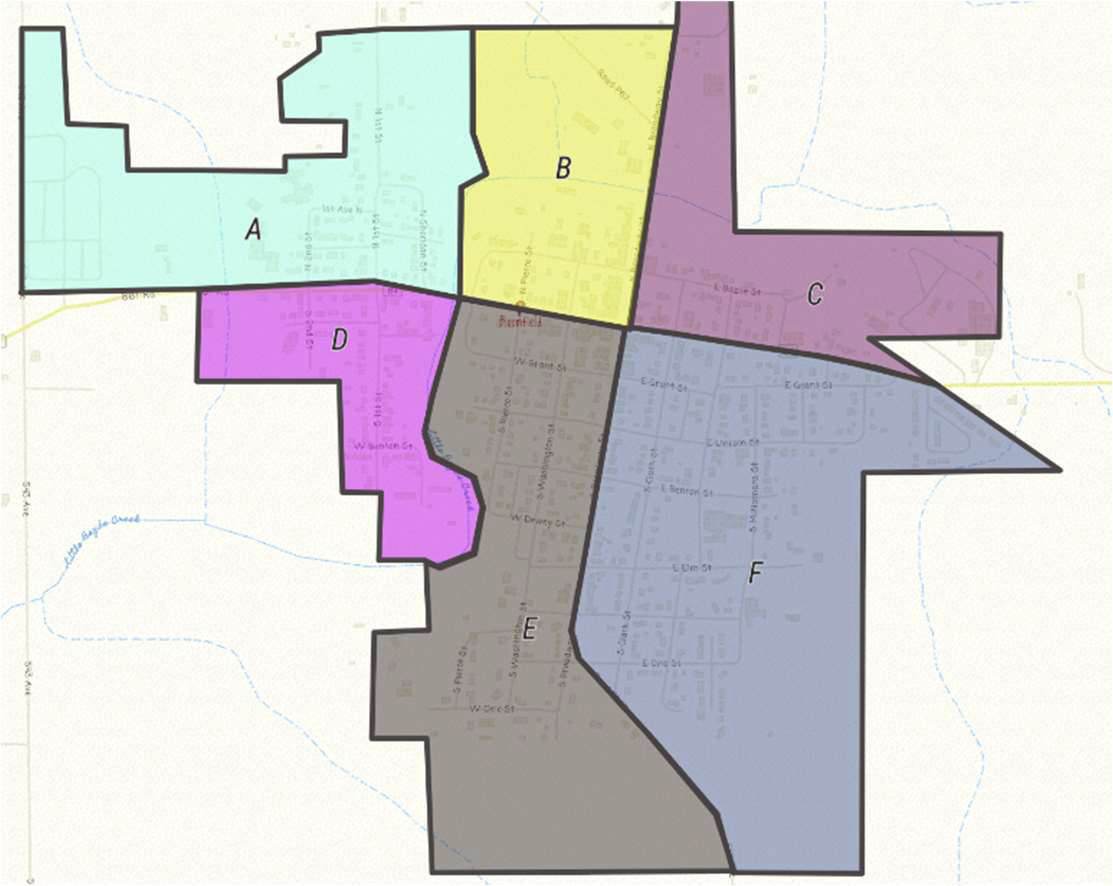
\includegraphics[width=\linewidth]{figures/community_survey_neighborhoods.png}
     \end{subfigure}
\end{framed}
\end{figure}

\noindent \hl{[survey summary toplines HERE]}

\pagebreak
\subsection{Future Land Use Map Workshop}

\noindent \hl{[is the online discussion on September 8 2025 the only one?]}

\section{Socioeconomic Data Curation}

\section{Map Development}

\section{Document Generation}



\label{EndOfText}
\end{document}
